\documentclass[preprint,12pt]{elsarticle}
\usepackage{iftex}
\ifPDFTeX
  \usepackage[T1]{fontenc}
  \usepackage[utf8]{inputenc}
  \usepackage{lmodern}
\else
  \usepackage[no-math]{fontspec}
\fi
\usepackage{amsmath}
\usepackage{amssymb}
\usepackage{amsfonts}
\usepackage{mathrsfs}
\usepackage{amsthm}
\usepackage{mathtools}
\usepackage{geometry}
\usepackage{enumitem}
\usepackage{longtable}
\usepackage{booktabs}
\usepackage{array}
\usepackage{microtype}
\usepackage{graphicx}
\graphicspath{{../figures/}{figures/}}
\usepackage[dvipsnames]{xcolor}
\usepackage{float}
\usepackage[pagebackref=true]{hyperref}
\usepackage{bookmark}
\usepackage{pdfcomment}

% Hover previews for internal references (no layout change).
\makeatletter
\let\CG@origref\ref
\let\CG@origeqref\eqref
\newcommand{\CG@gettip}[1]{\@ifundefined{CGTip@#1}{Reference: #1}{\csname CGTip@#1\endcsname}}
\DeclareRobustCommand{\CGref}[1]{\pdftooltip{\CG@origref{#1}}{\CG@gettip{#1}}}
\DeclareRobustCommand{\CGeqref}[1]{\pdftooltip{\CG@origeqref{#1}}{\CG@gettip{#1}}}
\makeatother
% Tooltip texts shown when hovering over internal references.
\makeatletter
\expandafter\gdef\csname CGTip@sec:introduction\endcsname{Section 1: Introduction (p. 2)}
\expandafter\gdef\csname CGTip@subsec:clock_intro\endcsname{Section 1.1: The Riemann--von Mangoldt clock and the ordinates (p. 2)}
\expandafter\gdef\csname CGTip@eq:intro_rvm\endcsname{Eq. (1.1), p. 2: N(T)=N\_0(T)+(1)/(pi)arg zeta ((1)/(2)+iT)+O((1)/(T)), N\_0(T)=(T)/(2pi)log(T)/(2pi e)+(7)/(8),}
\expandafter\gdef\csname CGTip@eq:intro_clock\endcsname{Eq. (1.2), p. 3: N\_0(tau\_k)=k-(1)/(2), tau\_k=(2pi (k-(11)/(8)))/(W\_0((k-(11)/(8))/e))(k>=1),}
\expandafter\gdef\csname CGTip@eq:intro_defect\endcsname{Eq. (1.3), p. 3: s\_k=k-(1)/(2)-N\_0(gamma\_k), u\_k(X)=s\_k-S\_X(gamma\_k), S\_X(t)=-(1)/(pi)sum\_p<= Xarg (1-p\textasciicircum{}-1/2-it).}
\expandafter\gdef\csname CGTip@subsec:known_intro\endcsname{Section 1.2: What is known and only used (p. 3)}
\expandafter\gdef\csname CGTip@subsec:main_results\endcsname{Section 1.3: What this paper adds (p. 3)}
\expandafter\gdef\csname CGTip@eq:intro_main\endcsname{Eq. (1.4), p. 4: (1)/(no.I\_T)sum\_kin I\_Tu\_k(X)\textasciicircum{}2=(1)/(2pi\textasciicircum{}2)log(1)/(c)+O(1+sqrt(log(1/c))).}
\expandafter\gdef\csname CGTip@sec:notation\endcsname{Section 2: Notation (p. 4)}
\expandafter\gdef\csname CGTip@subsec:symbols\endcsname{Section 2.1: List of symbols (p. 4)}
\expandafter\gdef\csname CGTip@subsec:counting\endcsname{Section 2.2: Counting functions (p. 6)}
\expandafter\gdef\csname CGTip@eq:RvM\endcsname{Eq. (2.1), p. 6: N(t)=(1)/(pi)vartheta(t)+1+S(t), S(t)=(1)/(pi)arg zeta ((1)/(2)+it)=O(log t),}
\expandafter\gdef\csname CGTip@eq:N0_def\endcsname{Eq. (2.2), p. 6: Theta\_0(t)=(t)/(2)log(t)/(2pi e)-(pi)/(8), N\_0(t)=(1)/(pi)Theta\_0(t)+1, varpi(t)=vartheta(t)-Theta\_0(t).}
\expandafter\gdef\csname CGTip@eq:N_decomposition\endcsname{Eq. (2.3), p. 6: N(t)=N\_0(t)+S(t)+(varpi(t))/(pi), L(t)=N\_0'(t)=(1)/(2pi)log(t)/(2pi).}
\expandafter\gdef\csname CGTip@eq:IT_size\endcsname{Eq. (2.4), p. 6: no.I\_T=TL(T)+O(T).}
\expandafter\gdef\csname CGTip@subsec:clock\endcsname{Section 2.3: The RvM clock and the displacements (p. 6)}
\expandafter\gdef\csname CGTip@eq:clock\endcsname{Eq. (2.5), p. 6: tau\_x=(2pi (x-(11)/(8)))/(W\_0((x-(11)/(8))/e)), (dtau\_x)/(dx)=(1)/(L(tau\_x))=(2pi)/(log(tau\_x/2pi)),}
\expandafter\gdef\csname CGTip@def:displacements\endcsname{Definition 2.1 (p. 7): For k>=1, s\_k=k-(1)/(2)-N\_0(gamma\_k) and delta\_k=tau\_k-gamma\_k.}
\expandafter\gdef\csname CGTip@eq:s_delta\endcsname{Eq. (2.6), p. 7: s\_k=L(xi\_k) delta\_kfor some xi\_k between gamma\_k and tau\_k .}
\expandafter\gdef\csname CGTip@lem:s_bounds\endcsname{Lemma 2.2 (p. 7): For every k>=1, N(gamma\_k\textasciicircum{}-)-N\_0(gamma\_k)+(1)/(2)<= s\_k<= N(gamma\_k\textasciicircum{}+)-N\_0(gamma\_k)-(1)/(2), and |s\_k|<=max(|S(gamma\_k\textasciicircum{}-)|,|S(gamma\_k\textasciicircum{}+)|)+(1)/(2)+(1)/(100).}
\expandafter\gdef\csname CGTip@eq:s_bounds\endcsname{Eq. (2.7), p. 7: N(gamma\_k\textasciicircum{}-)-N\_0(gamma\_k)+(1)/(2)<= s\_k<= N(gamma\_k\textasciicircum{}+)-N\_0(gamma\_k)-(1)/(2),}
\expandafter\gdef\csname CGTip@subsec:euler_phase\endcsname{Section 2.4: Euler phases and the corrected clock (p. 7)}
\expandafter\gdef\csname CGTip@eq:SA_def\endcsname{Eq. (2.8), p. 7: S\_A(t)=sum\_nin Aa\_nsin(tlog n), v\_A=(1)/(2)sum\_nin Aa\_n\textasciicircum{}2 ;}
\expandafter\gdef\csname CGTip@eq:SX_def\endcsname{Eq. (2.9), p. 7: S\_X(t)=-(1)/(pi)sum\_p<= Xarg (1-p\textasciicircum{}-1/2-it)=-(1)/(pi)sum\_p<= Xsum\_m>=1(sin(mtlog p))/(m p\textasciicircum{}m/2)=S\_A\_X(t).}
\expandafter\gdef\csname CGTip@eq:sigma_M_def\endcsname{Eq. (2.10), p. 7: |S\_X(t)|<=sigma\_X:=(1)/(pi)sum\_p<= Xsum\_m>=1(1)/(m p\textasciicircum{}m/2), |S\_X'(t)|<= M\_X:=(1)/(pi)sum\_p<= X(log p)/(sqrt(p)-1),}
\expandafter\gdef\csname CGTip@def:defect\endcsname{Definition 2.3 (p. 7): For X>=2 let F\_X=N\_0+S\_X and u\_k(X)=k-(1)/(2)-F\_X(gamma\_k)=s\_k-S\_X(gamma\_k). The one-step clock and its residual are tau\_k\textasciicircum{}X=tau\_k-(S\_X(tau\_k))/(L(tau\_k)), delta\_k\textasciicircum{}X=tau\_k\textasciicircum{}X-gamma\_k, r\_k(X)=L(tau\_k) delta\_k\textasciicircum{}X .}
\expandafter\gdef\csname CGTip@eq:one_step_clock\endcsname{Eq. (2.11), p. 7: tau\_k\textasciicircum{}X=tau\_k-(S\_X(tau\_k))/(L(tau\_k)), delta\_k\textasciicircum{}X=tau\_k\textasciicircum{}X-gamma\_k, r\_k(X)=L(tau\_k) delta\_k\textasciicircum{}X .}
\expandafter\gdef\csname CGTip@sec:known_results\endcsname{Section 3: External results (p. 8)}
\expandafter\gdef\csname CGTip@thm:known_basic\endcsname{Theorem 3.1 ([ref, Thms. 9.4, 9.9 and S 9.12], [ref]) (p. 8): S(t)=O(log t); gamma\_k+1-gamma\_k is bounded; and S\_1(t)=int\_0\textasciicircum{}tS(y) dy=O(log t).}
\expandafter\gdef\csname CGTip@thm:known_BW\endcsname{Theorem 3.2 (Bellotti--Wong [ref]) (p. 8): For T>= e, |N(T)-(T)/(2pi)log(T)/(2pi e)|<=BW(T).}
\expandafter\gdef\csname CGTip@thm:known_selberg_moments\endcsname{Theorem 3.3 (Selberg [ref]; see [ref, p. 225]) (p. 8): For every integer j>=1, int\_T\textasciicircum{}2TS(t)\textasciicircum{}2j dt=kappa\_j T(log log T)\textasciicircum{}j+O\_j(T(log log T)\textasciicircum{}j-1/2).}
\expandafter\gdef\csname CGTip@thm:known_korolev\endcsname{Theorem 3.4 (Selberg; Korolev [ref], [ref, Thm. 6]) (p. 8): Let Delta\_k be the integer such that g\_k+Delta\_k-1<gamma\_k<= g\_k+Delta\_k, and let 0<varepsilon\_0<10\textasciicircum{}-3. For every fixed j>=1, as n\_0->inf, sum\_n\_0<k<= n\_0+h\_0Delta\_k\textasciicircum{}2j=kappa\_jh\_0(log log n\_0)\textasciicircum{}j(1+o(1)) uniformly for n\_0\textasciicircum{}27/82+0.9varepsilon\_0<= h\_0<= n\_0\textasciicircum{}27/82+varepsilon\_0.}
\expandafter\gdef\csname CGTip@thm:known_selberg_approx\endcsname{Theorem 3.5 (Selberg's approximation in the form of Fujii [ref, S 3, pp. 232--233]) (p. 8): int\_T\textasciicircum{}2T(S(t)-S\textasciicircum{}rm pr\_Y\_0(t))\textasciicircum{}4dt<< T, where Y\_0=T\textasciicircum{}1/160.}
\expandafter\gdef\csname CGTip@thm:known_MV\endcsname{Theorem 3.6 (Montgomery--Vaughan [ref, Cor. 3]) (p. 8): For complex z\_n, int\_T\textasciicircum{}2T|sum\_n<= Yz\_nn\textasciicircum{}-it|\textasciicircum{}2dt=sum\_n<= Y|z\_n|\textasciicircum{}2(T+O(n)) with an absolute implied constant.}
\expandafter\gdef\csname CGTip@thm:known_mertens\endcsname{Theorem 3.7 (Mertens [ref]) (p. 8): For y>=2, sum\_p<= y(log p)/(p)=log y+O(1) and sum\_p<= y(1)/(p)=log log y+O(1).}
\expandafter\gdef\csname CGTip@thm:known_KL\endcsname{Theorem 3.8 (Kusmin--Landau [ref, Thm. 2.1]) (p. 8): Let Omega be real with continuous monotone derivative on [y\_1,y\_2] and ||Omega'||>=1/H\_rm KL>0 there, where ||*|| is the distance to the nearest integer. Then sum\_y\_1<n<= y\_2e\textasciicircum{}2pi iOmega(n)<< H\_rm KL.}
\expandafter\gdef\csname CGTip@thm:known_landau\endcsname{Theorem 3.9 (Landau [ref]; uniform version Gonek [ref]) (p. 8): For fixed integer n>=2, sum\_0<gamma <= tn\textasciicircum{}rho=-(t)/(2pi)Lambda(n)+O(log t), zeros counted with multiplicity.}
\expandafter\gdef\csname CGTip@rem:korolev\endcsname{Remark 3.10 (Known consequences for the clock) (p. 8): (a) Moments of s\_k. Since vartheta(gamma\_k)/pi in(k+Delta\_k-1,k+Delta\_k] and vartheta/pi=N\_0-1+varpi/pi, one has s\_k+Delta\_k=k+Delta\_k-(1)/(2)-N\_0(gamma\_k)in[-(3)/(2)+(varpi(gamma\_k))/(pi),-(1)/(2)+(varpi(gamma\_k))/(pi)), so |s\_k+Delta\_k|<2. The index set I\_T is the integer interval (N(T),N(2T)], of length \textasciitilde{} Tlog T....}
\expandafter\gdef\csname CGTip@eq:BW_pointwise\endcsname{Eq. (3.1), p. 9: -(BW(gamma\_k)+3/8)/(L(tau\_k))<=delta\_k<=(BW(gamma\_k)-11/8)/(L(gamma\_k))(k>=1).}
\expandafter\gdef\csname CGTip@sec:identities\endcsname{Section 4: Theorem A: an exact defect identity at the zeros (p. 9)}
\expandafter\gdef\csname CGTip@thm:identity_general\endcsname{Theorem 4.1 (p. 9): Let 1<= k\_1<k\_2 be indices, F a real C\textasciicircum{}1 function on an open interval containing [gamma\_k\_1,gamma\_k\_2], and u\_k=k-(1)/(2)-F(gamma\_k) for k\_1<= k<= k\_2. For every integer j>=1, int\_gamma\_k\_1\textasciicircum{}gamma\_k\_2(N(t)-F(t))\textasciicircum{}2jF'(t) dt=sum\_k=k\_1+1\textasciicircum{}k\_2-1Psi\_j(u\_k)+(((1)/(2)+u\_k\_1)\textasciicircum{}2j+1+((1)/(2)-u\_k\_2)\textasciicircum{}2j+1)/(2j+1), where Psi\_j(u)=...}
\expandafter\gdef\csname CGTip@eq:identity_general\endcsname{Eq. (4.1), p. 9: int\_gamma\_k\_1\textasciicircum{}gamma\_k\_2(N(t)-F(t))\textasciicircum{}2jF'(t) dt=sum\_k=k\_1+1\textasciicircum{}k\_2-1Psi\_j(u\_k)+(((1)/(2)+u\_k\_1)\textasciicircum{}2j+1+((1)/(2)-u\_k\_2)\textasciicircum{}2j+1)/(2j+1),}
\expandafter\gdef\csname CGTip@eq:Psi_def\endcsname{Eq. (4.2), p. 9: Psi\_j(u)=(((1)/(2)+u)\textasciicircum{}2j+1+((1)/(2)-u)\textasciicircum{}2j+1)/(2j+1)=sum\_l=0\textasciicircum{}jbinom(2j+1,2l)(4\textasciicircum{}l-j)/(2j+1) u\textasciicircum{}2l=u\textasciicircum{}2j+sum\_l<jbinom(2j+1,2l)(4\textasciicircum{}l-j)/(2j+1)u\textasciicircum{}2l.}
\expandafter\gdef\csname CGTip@eq:identity_quadratic\endcsname{Eq. (4.3), p. 9: sum\_k=k\_1+1\textasciicircum{}k\_2-1u\_k\textasciicircum{}2=int\_gamma\_k\_1\textasciicircum{}gamma\_k\_2(N(t)-F(t))\textasciicircum{}2F'(t) dt-(k\_2-k\_1-1)/(12)-(((1)/(2)+u\_k\_1)\textasciicircum{}3+((1)/(2)-u\_k\_2)\textasciicircum{}3)/(3) .}
\expandafter\gdef\csname CGTip@eq:identity_one_gap\endcsname{Eq. (4.4), p. 9: int\_gamma\_k\textasciicircum{}gamma\_k+1(k-F(t))\textasciicircum{}2jF'(t) dt =((k-F(gamma\_k))\textasciicircum{}2j+1-(k-F(gamma\_k+1))\textasciicircum{}2j+1)/(2j+1); =(((1)/(2)+u\_k)\textasciicircum{}2j+1+((1)/(2)-u\_k+1)\textasciicircum{}2j+1)/(2j+1),}
\expandafter\gdef\csname CGTip@rem:twelfth\endcsname{Remark 4.2 (p. 10): (1)/(12) is the mean square of a centred unit sawtooth: between consecutive zeros N-F decreases through one unit in the variable F(t). If F' changes sign, (4.3) remains exact with the integral counted with sign. With F=N\_0 and Theorem 3.3, induction on j through the lower-degree terms of Psi\_j recovers the moments o...}
\expandafter\gdef\csname CGTip@cor:identity_clock\endcsname{Corollary 4.3 (p. 10): For X>=2 and 1<= k\_1<k\_2, sum\_k=k\_1+1\textasciicircum{}k\_2-1u\_k(X)\textasciicircum{}2= int\_gamma\_k\_1\textasciicircum{}gamma\_k\_2(S-S\_X+(varpi)/(pi))\textasciicircum{}2(L+S\_X')dt; -(k\_2-k\_1-1)/(12)-(((1)/(2)+u\_k\_1(X))\textasciicircum{}3+((1)/(2)-u\_k\_2(X))\textasciicircum{}3)/(3) .}
\expandafter\gdef\csname CGTip@eq:identity_LeClair\endcsname{Eq. (4.5), p. 10: sum\_k=k\_1+1\textasciicircum{}k\_2-1u\_k(X)\textasciicircum{}2= int\_gamma\_k\_1\textasciicircum{}gamma\_k\_2(S-S\_X+(varpi)/(pi))\textasciicircum{}2(L+S\_X')dt; -(k\_2-k\_1-1)/(12)-(((1)/(2)+u\_k\_1(X))\textasciicircum{}3+((1)/(2)-u\_k\_2(X))\textasciicircum{}3)/(3) .}
\expandafter\gdef\csname CGTip@lem:first_moment_identity\endcsname{Lemma 4.4 (First-moment identity) (p. 10): Let 2pi<t\_1<t\_2 be points which are not ordinates and psi in C\textasciicircum{}1[t\_1,t\_2], real or complex. Then sum\_t\_1<gamma\_k<= t\_2s\_kpsi(gamma\_k)=int\_t\_1\textasciicircum{}t\_2G(t)psi(t)L(t) dt+(1)/(2)[psi G\textasciicircum{}2]\_t\_1\textasciicircum{}t\_2-(1)/(2)int\_t\_1\textasciicircum{}t\_2G(t)\textasciicircum{}2psi'(t) dt .}
\expandafter\gdef\csname CGTip@eq:first_moment_identity\endcsname{Eq. (4.6), p. 10: sum\_t\_1<gamma\_k<= t\_2s\_kpsi(gamma\_k)=int\_t\_1\textasciicircum{}t\_2G(t)psi(t)L(t) dt+(1)/(2)[psi G\textasciicircum{}2]\_t\_1\textasciicircum{}t\_2-(1)/(2)int\_t\_1\textasciicircum{}t\_2G(t)\textasciicircum{}2psi'(t) dt .}
\expandafter\gdef\csname CGTip@eq:first_moment_measures\endcsname{Eq. (4.7), p. 10: d(G\textasciicircum{}2)=-2GL dt+sum\_t\_1<gamma<t\_22G\textasciicircum{}*(gamma)nu(gamma) delta\_gamma ,}
\expandafter\gdef\csname CGTip@sec:main_theorem\endcsname{Section 5: Theorem B: how much prime information the clock needs (p. 11)}
\expandafter\gdef\csname CGTip@thm:main\endcsname{Theorem 5.1 (p. 11): There are absolute constants T\_0 and C such that for T>= T\_0 and every X with 2<= X<= T\textasciicircum{}1/2, writing c=log X/log T, |(1)/(no.I\_T)sum\_kin I\_Tu\_k(X)\textasciicircum{}2-(1)/(2pi\textasciicircum{}2)log(1)/(c)|<= C(1+sqrt(log(1/c))).}
\expandafter\gdef\csname CGTip@eq:main_theorem\endcsname{Eq. (5.1), p. 11: |(1)/(no.I\_T)sum\_kin I\_Tu\_k(X)\textasciicircum{}2-(1)/(2pi\textasciicircum{}2)log(1)/(c)|<= C(1+sqrt(log(1/c))).}
\expandafter\gdef\csname CGTip@cor:fixed_cutoff\endcsname{Corollary 5.2 (fixed cutoff) (p. 11): For fixed X>=2, (1)/(no.I\_T)sum\_kin I\_Tu\_k(X)\textasciicircum{}2=(1)/(2pi\textasciicircum{}2)log log T+O\_X(sqrt(log log T)), and no.kin I\_T:|u\_k(X)|<= y\_0=o(no.I\_T) for every fixed y\_0>0.}
\expandafter\gdef\csname CGTip@cor:power_cutoff\endcsname{Corollary 5.3 (power cutoff) (p. 11): For fixed 0<c<=(1)/(2) and X=T\textasciicircum{}c, limsup\_T->inf(1)/(no.I\_T)sum\_kin I\_Tu\_k(T\textasciicircum{}c)\textasciicircum{}2<=(1)/(2pi\textasciicircum{}2)log(1)/(c)+C(1+sqrt(log(1/c))), and no.kin I\_T:|u\_k(T\textasciicircum{}c)|>w\_T=o(no.I\_T) whenever w\_T->inf. The same holds for X=N(T)\textasciicircum{}c with fixed 0<c<(1)/(2), since then X=T\textasciicircum{}c' with c'=c+O(log log T/log T).}
\expandafter\gdef\csname CGTip@eq:power_cutoff\endcsname{Eq. (5.2), p. 11: limsup\_T->inf(1)/(no.I\_T)sum\_kin I\_Tu\_k(T\textasciicircum{}c)\textasciicircum{}2<=(1)/(2pi\textasciicircum{}2)log(1)/(c)+C(1+sqrt(log(1/c))),}
\expandafter\gdef\csname CGTip@cor:dichotomy\endcsname{Corollary 5.4 (dichotomy) (p. 11): Let X=X(T) with 2<= X<= T\textasciicircum{}1/2. The mean square of u\_k(X) over I\_T is bounded as T->inf if and only if liminf\_T->inflog X/log T>0. For fixed X\_0>=2 and cin(0,(1)/(2)], (1)/(no.I\_T)sum\_kin I\_T(u\_k(X\_0)\textasciicircum{}2-u\_k(T\textasciicircum{}c)\textasciicircum{}2)=(1)/(2pi\textasciicircum{}2)log log T+O(sqrt(log log T)) .}
\expandafter\gdef\csname CGTip@eq:dichotomy\endcsname{Eq. (5.3), p. 11: (1)/(no.I\_T)sum\_kin I\_T(u\_k(X\_0)\textasciicircum{}2-u\_k(T\textasciicircum{}c)\textasciicircum{}2)=(1)/(2pi\textasciicircum{}2)log log T+O(sqrt(log log T)) .}
\expandafter\gdef\csname CGTip@rem:comparison_LeClair\endcsname{Remark 5.5 (p. 11): Since logno.p<= X=log X+O(log log X), the condition of Corollary 5.4 says that the logarithm of the number of primes must grow proportionally to log T. A fixed number of primes, as in the computations of [ref, Sect. VI], leaves almost all zeros violating the corrected equation by more than any fixed amount; the requir...}
\expandafter\gdef\csname CGTip@rem:localization\endcsname{Remark 5.6 (Localization of the ordinates) (p. 12): If M\_X<=(1)/(2)L(T), then F\_X'>=L-M\_X>=(1)/(2)L(T) on [T,2T], so F\_X is strictly increasing there. For kin I\_T with F\_X(T)<= k-(1)/(2)<= F\_X(2T) the equation F\_X(t)=k-(1)/(2) has exactly one root t\_k\textasciicircum{}Xin[T,2T] (intermediate value theorem), and u\_k(X)=F\_X(t\_k\textasciicircum{}X)-F\_X(gamma\_k) gives |gamma\_k-t\_k\textasciicircum{}X|<=2|u\_k(X)|/L(T) (mea...}
\expandafter\gdef\csname CGTip@subsec:main_lemmas\endcsname{Section 5.1: Lemmas on prime polynomials (p. 12)}
\expandafter\gdef\csname CGTip@eq:D_def\endcsname{Eq. (5.4), p. 12: W\_1(t)=-(1)/(pi)sum\_pin J(sin(tlog p))/(sqrt(p)), V=sum\_pin J(1)/(p),; W=S\textasciicircum{}rm pr\_Y\_0-S\_X=+- W\_1-S\_X\textasciicircum{}(2)-S\_X\textasciicircum{}(>=3),}
\expandafter\gdef\csname CGTip@lem:V_size\endcsname{Lemma 5.7 (p. 12): V=log(1/c)+O(1) uniformly for log 2/log T<= c<=(1)/(2).}
\expandafter\gdef\csname CGTip@lem:trig_MV\endcsname{Lemma 5.8 (p. 12): For real z\_n, 2<= n<= Y, int\_T\textasciicircum{}2T(sum\_n<= Yz\_nsin(tlog n))\textasciicircum{}2dt=(T)/(2)sum\_n<= Yz\_n\textasciicircum{}2+O(sum\_n<= Ynz\_n\textasciicircum{}2+(sum\_n<= Y|z\_n|)\textasciicircum{}2), and the same with cos in place of sin.}
\expandafter\gdef\csname CGTip@eq:trig_MV\endcsname{Eq. (5.5), p. 12: int\_T\textasciicircum{}2T(sum\_n<= Yz\_nsin(tlog n))\textasciicircum{}2dt=(T)/(2)sum\_n<= Yz\_n\textasciicircum{}2+O(sum\_n<= Ynz\_n\textasciicircum{}2+(sum\_n<= Y|z\_n|)\textasciicircum{}2),}
\expandafter\gdef\csname CGTip@lem:D_moments\endcsname{Lemma 5.9 (p. 12): With absolute implied constants, int\_T\textasciicircum{}2T W\textasciicircum{}2 dt =(T)/(2pi\textasciicircum{}2)V+O(T(1+sqrt(V))), ; int\_T\textasciicircum{}2T W\textasciicircum{}4 dt << T(1+V)\textasciicircum{}2, ; int\_T\textasciicircum{}2TS\_X'(t)\textasciicircum{}2 dt << T(1+log X)\textasciicircum{}2 .}
\expandafter\gdef\csname CGTip@eq:D_second\endcsname{Eq. (5.6), p. 12: int\_T\textasciicircum{}2T W\textasciicircum{}2 dt =(T)/(2pi\textasciicircum{}2)V+O(T(1+sqrt(V))),}
\expandafter\gdef\csname CGTip@eq:D_fourth\endcsname{Eq. (5.7), p. 12: int\_T\textasciicircum{}2T W\textasciicircum{}4 dt << T(1+V)\textasciicircum{}2,}
\expandafter\gdef\csname CGTip@eq:SX_derivative\endcsname{Eq. (5.8), p. 12: int\_T\textasciicircum{}2TS\_X'(t)\textasciicircum{}2 dt << T(1+log X)\textasciicircum{}2 .}
\expandafter\gdef\csname CGTip@subsec:main_proof\endcsname{Section 5.2: Proof of Theorem 5.1 (p. 13)}
\expandafter\gdef\csname CGTip@eq:E0_bounds\endcsname{Eq. (5.9), p. 13: int\_T\textasciicircum{}2TE\_0\textasciicircum{}4 dt<< T,int\_T\textasciicircum{}2TE\_0\textasciicircum{}2 dt<= T\textasciicircum{}1/2(int\_T\textasciicircum{}2TE\_0\textasciicircum{}4 dt)\textasciicircum{}1/2<< T .}
\expandafter\gdef\csname CGTip@eq:J_asymptotic\endcsname{Eq. (5.10), p. 13: E\_2=(T)/(2pi\textasciicircum{}2)V+O(T(1+sqrt(V))),}
\expandafter\gdef\csname CGTip@eq:R_fourth\endcsname{Eq. (5.11), p. 13: int\_T\textasciicircum{}2TE\_X\textasciicircum{}4 dt<< T(1+V)\textasciicircum{}2 .}
\expandafter\gdef\csname CGTip@eq:main_step1\endcsname{Eq. (5.12), p. 13: sum\_kin I\_Tu\_k(X)\textasciicircum{}2=int\_T\textasciicircum{}2TE\_X\textasciicircum{}2L dt+int\_T\textasciicircum{}2TE\_X\textasciicircum{}2S\_X' dt-(no.I\_T)/(12)+O(T\textasciicircum{}3/4).}
\expandafter\gdef\csname CGTip@eq:main_step2\endcsname{Eq. (5.13), p. 13: |int\_T\textasciicircum{}2TE\_X\textasciicircum{}2S\_X' dt|<=(int\_T\textasciicircum{}2TE\_X\textasciicircum{}4)\textasciicircum{}1/2(int\_T\textasciicircum{}2TS\_X'\textasciicircum{}2)\textasciicircum{}1/2<< T(1+V)(1+log X).}
\expandafter\gdef\csname CGTip@eq:main_step3\endcsname{Eq. (5.14), p. 14: (1)/(no.I\_T)sum\_kin I\_Tu\_k(X)\textasciicircum{}2=(V)/(2pi\textasciicircum{}2)+O(1+sqrt(V)+(1+V)/(log T)+(1+V) c),}
\expandafter\gdef\csname CGTip@sec:accounting\endcsname{Section 6: Theorem C: exact accounting for the one-step clock (p. 14)}
\expandafter\gdef\csname CGTip@eq:two_responses\endcsname{Eq. (6.1), p. 14: R\textasciicircum{}gamma\_n(I)=(2)/(a\_n)< s\_ksin(gamma\_klog n)>\_I, R\textasciicircum{}tau\_n(I)=(2)/(a\_n)< s\_ksin(tau\_klog n)>\_I,}
\expandafter\gdef\csname CGTip@eq:Cr_def\endcsname{Eq. (6.2), p. 14: Cr\_A(I)=< S\_A(tau\_k)\textasciicircum{}2>\_I-v\_A .}
\expandafter\gdef\csname CGTip@thm:accounting\endcsname{Theorem 6.1 (Finite-window accounting) (p. 14): Let I be a finite nonempty set of indices and A a set of prime powers with sum\_nin A|a\_n|<inf. item For every k and X>=2, r\_k(X)=u\_k(X)+(S\_X(gamma\_k)-S\_X(tau\_k))+chi\_k,; |chi\_k|<=(delta\_k\textasciicircum{}2)/(2pi min(gamma\_k,tau\_k)),|S\_X(gamma\_k)-S\_X(tau\_k)|<= M\_X|delta\_k|. item For every real lambda, < s\_k\textasciicircum{}2-(s\_k-lambda S\_A(tau\_k))...}
\expandafter\gdef\csname CGTip@eq:one_step_decomposition\endcsname{Eq. (6.3), p. 14: r\_k(X)=u\_k(X)+(S\_X(gamma\_k)-S\_X(tau\_k))+chi\_k,; |chi\_k|<=(delta\_k\textasciicircum{}2)/(2pi min(gamma\_k,tau\_k)),|S\_X(gamma\_k)-S\_X(tau\_k)|<= M\_X|delta\_k|.}
\expandafter\gdef\csname CGTip@eq:exact_gain\endcsname{Eq. (6.4), p. 14: < s\_k\textasciicircum{}2-(s\_k-lambda S\_A(tau\_k))\textasciicircum{}2>\_I =sum\_nin Aa\_n\textasciicircum{}2(lambda R\textasciicircum{}tau\_n(I)-(lambda\textasciicircum{}2)/(2))-lambda\textasciicircum{}2Cr\_A(I).}
\expandafter\gdef\csname CGTip@eq:full_factor_gain\endcsname{Eq. (6.5), p. 14: < s\_k\textasciicircum{}2-(s\_k-S\_X(tau\_k))\textasciicircum{}2>\_I=D\_X(I)-Cr\_X(I),; D\_X(I)=sum\_nin A\_Xa\_n\textasciicircum{}2(R\textasciicircum{}tau\_n(I)-(1)/(2))=2< s\_kS\_X(tau\_k)>\_I-v\_X,}
\expandafter\gdef\csname CGTip@rem:accounting_meaning\endcsname{Remark 6.2 (p. 15): (6.5) is an exact sign criterion for the gain of the full Euler phase at the clock points: the gain is positive exactly when the diagonal responses outweigh the cross term. No independence of the phases tau\_klog p is assumed. A threshold R\textasciicircum{}tau\_p=(1)/(2) describes a single diagonal prime contribution and does not det...}
\expandafter\gdef\csname CGTip@rem:matrix_projection\endcsname{Remark 6.3 (Optimal trigonometric correction) (p. 15): For a finite set A of frequencies let varsigma\_n(k)=sin(tau\_klog n), Q=(<varsigma\_n\_1varsigma\_n\_2>\_I)\_n\_1,n\_2in A, b=(< s\_kvarsigma\_n(k)>\_I)\_nin A and Upsilon\_lambda=sum\_nlambda\_nvarsigma\_n. Ordinary least squares gives <(s\_k-Upsilon\_lambda(k))\textasciicircum{}2>\_I=< s\_k\textasciicircum{}2>\_I-2lambda\textasciicircum{} T b+lambda\textasciicircum{} T Qlambda, minimized by lambda= Q\textasciicircum{}d...}
\expandafter\gdef\csname CGTip@rem:transport\endcsname{Remark 6.4 (Clock point against zero) (p. 15): For a prime power n, sin(gamma\_kl\_n)-sin(tau\_kl\_n)=int\_0\textasciicircum{}1(d)/(dy)sin((tau\_k-ydelta\_k)l\_n) dy, whence, exchanging the finite mean and the integral, R\textasciicircum{}gamma\_n(I)-R\textasciicircum{}tau\_n(I)=-(2l\_n)/(a\_n)int\_0\textasciicircum{}1< s\_kdelta\_kcos ((tau\_k-ydelta\_k)l\_n)>\_I dy . For fixed n and I=I\_T the right side is O(<|s\_kdelta\_k|>\_I\_T)=O(log log T/log T...}
\expandafter\gdef\csname CGTip@eq:response_transport\endcsname{Eq. (6.6), p. 15: R\textasciicircum{}gamma\_n(I)-R\textasciicircum{}tau\_n(I)=-(2l\_n)/(a\_n)int\_0\textasciicircum{}1< s\_kdelta\_kcos ((tau\_k-ydelta\_k)l\_n)>\_I dy .}
\expandafter\gdef\csname CGTip@rem:fixed_sup\endcsname{Remark 6.5 (Fixed prime sets) (p. 15): For fixed X, |delta\_k\textasciicircum{}X-delta\_k|<=sigma\_X/L(tau\_k)->0 and |u\_k(X)-s\_k|<=sigma\_X. A fixed set of primes changes neither limsup\_k|delta\_k| nor the unboundedness of the defect.}
\expandafter\gdef\csname CGTip@sec:computations\endcsname{Section 7: Computations (p. 15)}
\expandafter\gdef\csname CGTip@subsec:data\endcsname{Section 7.1: Data and methods (p. 15)}
\expandafter\gdef\csname CGTip@subsec:clock_data\endcsname{Section 7.2: The clock and the ordinates (p. 16)}
\expandafter\gdef\csname CGTip@fig:displacement\endcsname{Figure 1 (p. 16): The displacement delta\_k=tau\_k-gamma\_k of the RvM clock and the residual tau\_k\textasciicircum{}PP-gamma\_k of the one-step clock with PP=2,3,5,7 and saturation B=0.6, for k<=2000.}
\expandafter\gdef\csname CGTip@subsec:direct_defects\endcsname{Section 7.3: Direct defects (Theorem B) (p. 16)}
\expandafter\gdef\csname CGTip@tab:direct\endcsname{Table 2 (p. 17): Mean squares of the defect u\_k(X) and of the one-step residual r\_k(X) over T<gamma\_k<=2T, X=T\textasciicircum{}c.}
\expandafter\gdef\csname CGTip@fig:direct_defects\endcsname{Figure 2 (p. 17): Mean square of u\_k(X) (filled markers) and of r\_k(X) (open markers) over T<gamma\_k<=2T against log(1/c), X=T\textasciicircum{}c, for the four heights of Table 2; dashed: (1)/(2pi\textasciicircum{}2)log(1/c).}
\expandafter\gdef\csname CGTip@subsec:accounting_data\endcsname{Section 7.4: Exact accounting (Theorem C) (p. 19)}
\expandafter\gdef\csname CGTip@tab:accounting\endcsname{Table 3 (p. 18): Exact decomposition (6.5) of the one-step gain into the diagonal term D\_X and the cross term Cr\_X.}
\expandafter\gdef\csname CGTip@fig:accounting\endcsname{Figure 3 (p. 18): Gain of the one-step clock (filled markers) and cross term Cr\_X (open markers) against the cutoff X, for five windows of ordinals; dashed: v\_X.}
\expandafter\gdef\csname CGTip@subsec:one_step_cutoff\endcsname{Section 7.5: The one-step clock against the cutoff (p. 19)}
\expandafter\gdef\csname CGTip@tab:methods\endcsname{Table 4 (p. 19): Root mean square, maximum of |tau\_k\textasciicircum{}X-gamma\_k| and number of residuals >=(1)/(2) over all K ordinates, and the same quantities in the top window (10\textasciicircum{}6,K].}
\expandafter\gdef\csname CGTip@fig:rms_cutoff\endcsname{Figure 4 (p. 20): Root mean square of tau\_k\textasciicircum{}X-gamma\_k (no saturation) against the cutoff X, by window of ordinals; dots mark the minimum in each window.}
\expandafter\gdef\csname CGTip@fig:max_window\endcsname{Figure 5 (p. 20): Maximum of |tau\_k\textasciicircum{}X-gamma\_k| in each window of ordinals for the five rules of Table 4; dotted: (1)/(2).}
\expandafter\gdef\csname CGTip@sec:conditional\endcsname{Section 8: Conditional results (p. 19)}
\expandafter\gdef\csname CGTip@subsec:hypL\endcsname{Section 8.1: Fixed frequencies under Hypothesis L (p. 19)}
\expandafter\gdef\csname CGTip@hyp:L\endcsname{Hypothesis 8.1 (Hypothesis L: fixed-frequency Landau formula on the critical line) (p. 19): For every fixed integer n>=2, sum\_0<gamma <= tn\textasciicircum{}igamma=-(t)/(2pi)(Lambda(n))/(sqrt(n))+o(t), the zeros of the Riemann zeta function being counted with multiplicity.}
\expandafter\gdef\csname CGTip@prop:L_sufficient\endcsname{Proposition 8.2 (p. 19): Hypothesis L holds if sum\_0<gamma <= t|beta-(1)/(2)|=o(t).}
\expandafter\gdef\csname CGTip@lem:clock_equidistribution\endcsname{Lemma 8.3 (p. 21): For fixed real omega !=0, sum\_kin I\_Te\textasciicircum{}iomega tau\_k<<\_omega log T. Hence for fixed integers n\_1,n\_2>=2, <sin(tau\_klog n\_1)sin(tau\_klog n\_2)>\_I\_T->(1)/(2) 1\_n\_1=n\_2.}
\expandafter\gdef\csname CGTip@thm:projection\endcsname{Theorem 8.4 (Under Hypothesis L) (p. 21): Assume Hypothesis L. For every fixed integer n>=2, < s\_ksin(gamma\_klog n)>\_I\_T->(a\_n)/(2), and the same with tau\_k in place of gamma\_k; thus R\textasciicircum{}gamma\_n(I\_T),R\textasciicircum{}tau\_n(I\_T)->1 for prime powers n.}
\expandafter\gdef\csname CGTip@eq:projection_Phi\endcsname{Eq. (8.1), p. 21: H\_n(t)=[(S(y)n\textasciicircum{}iy)/(il\_n)]\_14\textasciicircum{}t-(1)/(il\_n)sum\_14<gamma\_k<= tn\textasciicircum{}igamma\_k+(1)/(il\_n)int\_14\textasciicircum{}tn\textasciicircum{}iy(L+(varpi')/(pi))dy=(i)/(l\_n)sum\_0<gamma\_k<= tn\textasciicircum{}igamma\_k+O(log t),}
\expandafter\gdef\csname CGTip@eq:projection_partial\endcsname{Eq. (8.2), p. 21: int\_T\textasciicircum{}2TS(t)n\textasciicircum{}itL(t) dt=[ H\_nL ]\_T\textasciicircum{}2T-int\_T\textasciicircum{}2T(H\_n(t))/(2pi t) dt=-i(Lambda(n))/(2pisqrt(n) l\_n)int\_T\textasciicircum{}2TL dt+o(Tlog T).}
\expandafter\gdef\csname CGTip@cor:gain\endcsname{Corollary 8.5 (Under Hypothesis L) (p. 21): For a finite set A of prime powers and lambda in R, < s\_k\textasciicircum{}2-(s\_k-lambda S\_A(tau\_k))\textasciicircum{}2>\_I\_T->(2lambda-lambda\textasciicircum{}2)v\_A, maximal at lambda=1.}
\expandafter\gdef\csname CGTip@fig:gain_fixed\endcsname{Figure 6 (p. 22): Mean-square gain < s\_k\textasciicircum{}2>-<(s\_k-S\_PP(tau\_k))\textasciicircum{}2> of two fixed prime sets PP (full local factors) in each window of ordinals, and the constants v\_PP (dashed) of Corollary 8.5.}
\expandafter\gdef\csname CGTip@subsec:gamma_response\endcsname{Section 8.2: The response at the ordinates and its Fourier reduction (p. 22)}
\expandafter\gdef\csname CGTip@eq:ATp_STp\endcsname{Eq. (8.3), p. 22: A\_T,p=-(2pisqrt(p))/(no.I\_T)int\_T\textasciicircum{}2TG(t)sin(tlog p)L(t) dt, S\_T,p=(1)/(T)int\_T\textasciicircum{}2TS(t)\textasciicircum{}2p\textasciicircum{}it dt.}
\expandafter\gdef\csname CGTip@prop:gamma_response_exact\endcsname{Proposition 8.6 (Unconditional separation of one- and two-point terms) (p. 22): R\textasciicircum{}gamma\_p(I\_T)= A\_T,p+(pisqrt(p) Tlog p)/(no.I\_T)Re S\_T,p-(pisqrt(p))/(no.I\_T)[G\textasciicircum{}2sin(tlog p)]\_T\textasciicircum{}2T; +(pisqrt(p)log p)/(no.I\_T)int\_T\textasciicircum{}2T(G\textasciicircum{}2-S\textasciicircum{}2)cos(tlog p) dt. If theta=log p/L\_T stays in a compact subset of (0,1), the last two terms are o(1) and R\textasciicircum{}gamma\_p(I\_T)= A\_T,p+2pi\textasciicircum{}2thetasqrt(p) (1+O(1/L\_T))Re S\_T,p+o(1).}
\expandafter\gdef\csname CGTip@eq:gamma_response_exact\endcsname{Eq. (8.4), p. 22: R\textasciicircum{}gamma\_p(I\_T)= A\_T,p+(pisqrt(p) Tlog p)/(no.I\_T)Re S\_T,p-(pisqrt(p))/(no.I\_T)[G\textasciicircum{}2sin(tlog p)]\_T\textasciicircum{}2T; +(pisqrt(p)log p)/(no.I\_T)int\_T\textasciicircum{}2T(G\textasciicircum{}2-S\textasciicircum{}2)cos(tlog p) dt.}
\expandafter\gdef\csname CGTip@eq:gamma_response_scaled\endcsname{Eq. (8.5), p. 22: R\textasciicircum{}gamma\_p(I\_T)= A\_T,p+2pi\textasciicircum{}2thetasqrt(p) (1+O(1/L\_T))Re S\_T,p+o(1).}
\expandafter\gdef\csname CGTip@eq:measure_def\endcsname{Eq. (8.6), p. 22: Z\_T(omega)=int\_R e\textasciicircum{}iomega t d m\_T(t), hat f\_T(omega)=int\_R f\_T(t)e\textasciicircum{}iomega tdt .}
\expandafter\gdef\csname CGTip@thm:Fourier_exact\endcsname{Theorem 8.7 (Unconditional shifted two-point representation) (p. 23): For non-ordinates T,2T, Z\_T(omega)=sum\_T<gamma<2Tnu(gamma)e\textasciicircum{}iomega gamma-int\_T\textasciicircum{}2T(L(t)+(varpi'(t))/(pi))e\textasciicircum{}iomega t dt+S(T)e\textasciicircum{}iomega T-S(2T)e\textasciicircum{}2iomega T, Z\_T(omega)=-iomega hat f\_T(omega), so that Z\_T(0)=0 and Z\_T(omega)/omega extends continuously by -ihat f\_T; and for every real omega\_0 int\_T\textasciicircum{}2TS(t)\textasciicircum{}2e\textasciicircum{}iomega\_0t dt=-(...}
\expandafter\gdef\csname CGTip@eq:measure_expansion\endcsname{Eq. (8.7), p. 23: Z\_T(omega)=sum\_T<gamma<2Tnu(gamma)e\textasciicircum{}iomega gamma-int\_T\textasciicircum{}2T(L(t)+(varpi'(t))/(pi))e\textasciicircum{}iomega t dt+S(T)e\textasciicircum{}iomega T-S(2T)e\textasciicircum{}2iomega T,}
\expandafter\gdef\csname CGTip@eq:Fourier_convolution\endcsname{Eq. (8.8), p. 23: int\_T\textasciicircum{}2TS(t)\textasciicircum{}2e\textasciicircum{}iomega\_0t dt=-(1)/(2pi)int\_R(Z\_T(omega)Z\_T(omega\_0-omega))/(omega(omega\_0-omega)) domega,}
\expandafter\gdef\csname CGTip@eq:BT_scaled\endcsname{Eq. (8.9), p. 23: B\_T(theta)=int\_R(Z\_T(alpha L\_T)Z\_T((theta-alpha)L\_T))/(alpha(theta-alpha)) dalpha,so that S\_T,p=-(B\_T(theta))/(2pi TL\_T).}
\expandafter\gdef\csname CGTip@subsec:kernel\endcsname{Section 8.3: The kernel K\_theta (p. 23)}
\expandafter\gdef\csname CGTip@eq:kernel_piecewise\endcsname{Eq. (8.10), p. 23: K\_theta(alpha)= theta, alpha <=-1,; theta-1-alpha, -1<=alpha <=theta-1,; 0, theta-1<=alpha <=1,; alpha-1, 1<=alpha <=1+theta,; theta, alpha >=1+theta,}
\expandafter\gdef\csname CGTip@eq:kernel_intersections\endcsname{Eq. (8.11), p. 23: K\_theta(alpha)=1-h(alpha)-h(theta-alpha)-h(theta)+2max (1-max(|alpha|,|theta-alpha|,theta),0),}
\expandafter\gdef\csname CGTip@prop:kernel_integral\endcsname{Proposition 8.8 (Integral and support of the kernel) (p. 23): For 0<theta<1, int\_R(K\_theta(alpha))/(alpha(theta-alpha)) dalpha=-(2Phi(theta))/(theta), the integral being absolutely convergent, and K\_theta(alpha)=0 whenever |alpha|+|theta-alpha|+theta<2.}
\expandafter\gdef\csname CGTip@eq:kernel_integral\endcsname{Eq. (8.12), p. 23: int\_R(K\_theta(alpha))/(alpha(theta-alpha)) dalpha=-(2Phi(theta))/(theta),}
\expandafter\gdef\csname CGTip@subsec:conditional_law\endcsname{Section 8.4: The moving-prime law under Hypotheses U and W (p. 24)}
\expandafter\gdef\csname CGTip@hyp:uniform_prime\endcsname{Hypothesis 8.9 (Hypothesis U: uniform one-particle input) (p. 24): For every 0<theta\_0<theta\_1<1, uniformly for primes with theta\_0<=log p/L\_T<=theta\_1, A\_T,p=1+o(1).}
\expandafter\gdef\csname CGTip@hyp:weighted_bridge\endcsname{Hypothesis 8.10 (Hypothesis W: weighted arithmetic bridge) (p. 24): Uniformly for primes with theta in any compact subset of (0,1), int\_R(Z\_T(alpha L\_T)Z\_T((theta-alpha)L\_T)+ N\_Tp\textasciicircum{}-1/2 K\_theta(alpha))/(alpha(theta-alpha)) dalpha=o((TL\_T)/(sqrt(p))), with the continuous extensions of Z\_T(omega)/omega at omega=0.}
\expandafter\gdef\csname CGTip@eq:weighted_arithmetic_bridge\endcsname{Eq. (8.13), p. 24: int\_R(Z\_T(alpha L\_T)Z\_T((theta-alpha)L\_T)+ N\_Tp\textasciicircum{}-1/2 K\_theta(alpha))/(alpha(theta-alpha)) dalpha=o((TL\_T)/(sqrt(p))),}
\expandafter\gdef\csname CGTip@prop:conditional_universal\endcsname{Proposition 8.11 (Moving-prime law under Hypotheses U and W) (p. 24): Under Hypothesis W, S\_T,p=-(1)/(2pi\textasciicircum{}2sqrt(p))(Phi(theta))/(theta)+o(p\textasciicircum{}-1/2). Under Hypotheses U and W, or U and the real part of (8.14), uniformly for theta in compact subsets of (0,1), R\textasciicircum{}gamma\_p(I\_T)=1-Phi(theta)+o(1). Conversely, under Hypothesis U, (8.15) is equivalent to the real part of (8.14). Nothing is asser...}
\expandafter\gdef\csname CGTip@eq:CTp_target\endcsname{Eq. (8.14), p. 24: S\_T,p=-(1)/(2pi\textasciicircum{}2sqrt(p))(Phi(theta))/(theta)+o(p\textasciicircum{}-1/2).}
\expandafter\gdef\csname CGTip@eq:conditional_universal\endcsname{Eq. (8.15), p. 24: R\textasciicircum{}gamma\_p(I\_T)=1-Phi(theta)+o(1).}
\expandafter\gdef\csname CGTip@rem:scale_gap\endcsname{Remark 8.12 (p. 24): Phi(theta)=2sum\_j>=1(theta\textasciicircum{}2j)/((2j-1)2j)=theta\textasciicircum{}2+(theta\textasciicircum{}4)/(6)+(theta\textasciicircum{}6)/(15)+..., so 1-theta\textasciicircum{}2 is only the quadratic truncation of (8.15), and 1-Phi(theta) vanishes at theta=0.9036.... Hypotheses U and W are not consequences of Hypothesis L. The prime polynomial alone does not give (8.14): writing S=S\textasciicircum{}rm pr\_Y+(S-S...}
\expandafter\gdef\csname CGTip@sec:heuristic\endcsname{Section 9: Heuristic support and numerical evidence (p. 25)}
\expandafter\gdef\csname CGTip@subsec:det_model\endcsname{Section 9.1: A determinantal model whose connected kernel is K\_theta (p. 25)}
\expandafter\gdef\csname CGTip@eq:real_tilt\endcsname{Eq. (9.1), p. 25: d P\_iota\_1,iota\_2=(exp -iota\_1Re Xi\_-theta-iota\_2Im Xi\_-theta)/(Eexp -iota\_1Re Xi\_-theta-iota\_2Im Xi\_-theta) d P\_0,0}
\expandafter\gdef\csname CGTip@thm:sine_kernel\endcsname{Theorem 9.1 (Connected kernel of the model) (p. 25): Let lattice frequencies tend to alpha,theta-alpha,-theta with 0<theta<1. Then R\_0\textasciicircum{}-1cum\_3(Xi\_alpha,Xi\_theta-alpha,Xi\_-theta)-> K\_theta(alpha) and R\_0\textasciicircum{}-1cum\_2(Xi\_theta,Xi\_-theta)->theta.}
\expandafter\gdef\csname CGTip@eq:third_cumulant_trace\endcsname{Eq. (9.2), p. 25: cum\_3= Tr(m\_1 m\_2 m\_3Pi\_ n)-Tr(m\_1 m\_2Pi\_ n m\_3Pi\_ n)-Tr(m\_1 m\_3Pi\_ n m\_2Pi\_ n)-Tr(m\_2 m\_3Pi\_ n m\_1Pi\_ n); +Tr(m\_1Pi\_ n m\_2Pi\_ n m\_3Pi\_ n)+Tr(m\_1Pi\_ n m\_3Pi\_ n m\_2Pi\_ n),}
\expandafter\gdef\csname CGTip@subsec:numerics_law\endcsname{Section 9.2: Numerical evidence (p. 26)}
\expandafter\gdef\csname CGTip@conj:law\endcsname{Conjecture 9.2 (p. 26): For primes with theta=log p/L\_T in compact subsets of (0,1), R\textasciicircum{}gamma\_p(I\_T)=1-Phi(theta)+o(1).}
\expandafter\gdef\csname CGTip@tab:response_errors\endcsname{Table 5 (p. 26): Errors of R\textasciicircum{}gamma\_p-(1-Phi(theta)) over the primes p<=20 000 with theta<1.}
\expandafter\gdef\csname CGTip@tab:response_bins\endcsname{Table 6 (p. 27): Bin means of R\textasciicircum{}gamma\_p and R\textasciicircum{}tau\_p in the two top windows; ``law'' is the mean of 1-Phi(theta) over the same primes, s.e. the standard error of the mean difference.}
\expandafter\gdef\csname CGTip@fig:response_law\endcsname{Figure 7 (p. 26): Bin means of R\textasciicircum{}gamma\_p (bars: standard error) against 1-Phi(theta) (solid) and 1-theta\textasciicircum{}2 (dashed), for five windows of ordinals.}
\expandafter\gdef\csname CGTip@fig:response_clock\endcsname{Figure 8 (p. 28): Bin means of the response at the clock points, R\textasciicircum{}tau\_p (squares), and at the zeros, R\textasciicircum{}gamma\_p (circles), for three windows of ordinals; solid: 1-Phi(theta).}
\expandafter\gdef\csname CGTip@sec:conclusions\endcsname{Section 10: Conclusions (p. 28)}
\expandafter\gdef\csname CGTip@q:constant\endcsname{Question 10.1 (p. 29): For fixed cin(0,(1)/(2)], do the bounded means of u\_k(T\textasciicircum{}c)\textasciicircum{}2 converge, and to (2pi\textasciicircum{}2)\textasciicircum{}-1log(1/c) plus which constant? This needs the mixed Selberg remainders and the prime-power terms, not only upper bounds.}
\expandafter\gdef\csname CGTip@q:large_c\endcsname{Question 10.2 (p. 29): Can Theorem 5.1 be extended to c>(1)/(2) (the proof uses X\textasciicircum{}2<= T in the fourth-moment step), and to a cutoff varying at every ordinate, such as X\_k=(tau\_k/2pi)\textasciicircum{}c?}
\expandafter\gdef\csname CGTip@q:prime_bridge\endcsname{Question 10.3 (p. 29): Can Hypotheses U and W be proved for moving primes, in the real or the complex form? What is the finite-height correction to 1-Phi(theta) seen in Table 6? Is there a law for the response R\textasciicircum{}tau at the clock points, with uniform control of the Gram matrix of Remark 6.3, that would predict the optimal cutoff of the com...}
\makeatother

\hypersetup{
  colorlinks=false,
  pdfborder={0 0 1},
  linkbordercolor={1 0 0},
  citebordercolor={0 0.3 1},
  urlbordercolor={0 0.6 0.6},
  filebordercolor={0 0.6 0.6},
  linktoc=all,
  bookmarksnumbered=true,
  bookmarksopen=true,
  bookmarksopenlevel=1,
  pdfstartview=FitH,
  pdftitle={The Riemann-von Mangoldt clock and the zeros of the Riemann zeta function: an exact defect identity and variable prime cutoffs},
  pdfauthor={Rotkiv Ayn\"asac},
  pdfsubject={Zeros of the Riemann zeta function, Riemann-von Mangoldt clock, ordinal defect, truncated Euler products, prime cutoff},
  pdfkeywords={Riemann zeta function, zeros of the Riemann zeta function, Riemann-von Mangoldt formula, argument of the Riemann zeta function, Euler product, prime cutoff}
}
% Back-references in the bibliography.
\renewcommand*{\backref}[1]{}
\renewcommand*{\backrefalt}[4]{%
  \ifcase #1 %
    \relax
  \or
    \ (Cited on p.~#2.)%
  \else
    \ (Cited on pp.~#2.)%
  \fi}

\geometry{margin=1in}
\numberwithin{equation}{section}
\setcounter{tocdepth}{2}
\setcounter{secnumdepth}{3}
\setlength{\emergencystretch}{1.5em}

\theoremstyle{plain}
\newtheorem{theorem}{Theorem}[section]
\newtheorem{proposition}[theorem]{Proposition}
\newtheorem{lemma}[theorem]{Lemma}
\newtheorem{corollary}[theorem]{Corollary}
\newtheorem{conjecture}[theorem]{Conjecture}
\theoremstyle{definition}
\newtheorem{definition}[theorem]{Definition}
\newtheorem{hypothesis}[theorem]{Hypothesis}
\newtheorem{question}[theorem]{Question}
\theoremstyle{remark}
\newtheorem{remark}[theorem]{Remark}

\newcommand{\R}{\mathbb R}
\newcommand{\NO}{N_0}
\newcommand{\lL}{\mathcal L}
\newcommand{\IT}{\mathcal I_T}
\newcommand{\sgn}{\operatorname{sgn}}
\newcommand{\Cr}{\operatorname{Cr}}
\newcommand{\BW}{\operatorname{BW}}
\newcommand{\Rg}{\mathcal R^{\gamma}}
\newcommand{\Rt}{\mathcal R^{\tau}}
\newcommand{\PP}{\mathcal P}

\begin{document}

\begin{frontmatter}
\title{The Riemann--von Mangoldt clock and the zeros of the Riemann zeta function: an exact defect identity and variable prime cutoffs}
\author{Rotkiv Ayn\"asac}

\begin{abstract}
Let $\gamma_k$ be the ordinates of the nontrivial zeros of the Riemann zeta function, counted with multiplicity, and let $\tau_k$ be the midpoint Riemann--von Mangoldt clock, defined by $\NO(\tau_k)=k-\frac12$, where $\NO$ is the smooth part of the Riemann--von Mangoldt formula. \emph{Known:} $\limsup_k|\tau_k-\gamma_k|\le0.6331$ follows from the bound of Bellotti and Wong for the argument of the Riemann zeta function, and the ordinal displacement $s_k=k-\frac12-\NO(\gamma_k)$ has Gaussian moments of variance $\frac1{2\pi^2}\log\log T$ by Selberg's formulae proved by Korolev. \emph{New:} (A) for every $C^1$ model $F$ of the zero-counting function, sums of even powers of $k-\frac12-F(\gamma_k)$ over consecutive ordinates equal weighted integrals of $N-F$ minus explicit sawtooth and boundary terms, with no hypothesis on the zeros; (B) if the clock equation is corrected by the Euler phase $S_X$ of the primes $p\le X$, the mean square over $T<\gamma_k\le2T$ of the defect $u_k(X)=k-\frac12-\NO(\gamma_k)-S_X(\gamma_k)$ is $\frac1{2\pi^2}\log\frac{\log T}{\log X}+O(1+\sqrt{\log\frac{\log T}{\log X}})$ uniformly for $2\le X\le T^{1/2}$, so the corrected clock places almost all zeros within a bounded number of positions if and only if $\log X\gg\log T$; (C) the mean-square gain of the computable one-step corrected clock on any finite set of zeros is, exactly, a diagonal prime-response term minus a cross term, which accounts for the cutoff that is optimal at a given height. Under two named hypotheses the prime response of $s_k$ at the zeros is $1-\Phi(\theta)$, $\Phi(\theta)=(1+\theta)\log(1+\theta)+(1-\theta)\log(1-\theta)$, $\theta=\log p/\log(T/2\pi)$; a determinantal model motivating one hypothesis is kept separate. The observables of (B) and (C) are computed on the first $2\,001\,052$ zeros of the Riemann zeta function.
\end{abstract}

\begin{keyword}
Riemann zeta function \sep zeros of the Riemann zeta function \sep Riemann--von Mangoldt formula \sep argument of the Riemann zeta function \sep truncated Euler product
\MSC[2020] 11M06 \sep 11M26 \sep 11Y35
\end{keyword}
\end{frontmatter}

\tableofcontents

%======================================================================
\section{Introduction}
\label{sec:introduction}

\subsection{The Riemann--von Mangoldt clock and the ordinates}
\label{subsec:clock_intro}
Let $\zeta(s)$ be the Riemann zeta function, let $N(T)$ be the number of its nontrivial zeros $\rho=\beta+i\gamma$ with $0<\gamma\le T$, counted with multiplicity, and list their ordinates as $\gamma_1\le\gamma_2\le\cdots$, with multiplicity. Away from ordinates the Riemann--von Mangoldt formula reads \cite[\S\S9.3--9.4]{Titchmarsh1986}
\begin{equation}
 N(T)=\NO(T)+\frac1\pi\arg\zeta\Bigl(\frac12+iT\Bigr)+O\Bigl(\frac1T\Bigr),\qquad \NO(T)=\frac{T}{2\pi}\log\frac{T}{2\pi e}+\frac78,
 \label{eq:intro_rvm}
\end{equation}
the argument of the Riemann zeta function being obtained by continuous variation along $2\to2+iT\to\frac12+iT$ from $\arg\zeta(2)=0$. The \emph{midpoint Riemann--von Mangoldt clock} (RvM clock) is the sequence $\tau_k$ defined by
\begin{equation}
 \NO(\tau_k)=k-\frac12,\qquad \tau_k=\frac{2\pi\,(k-\frac{11}8)}{W_0\bigl((k-\frac{11}8)/e\bigr)}\qquad(k\ge1),
 \label{eq:intro_clock}
\end{equation}
where $W_0$ is the principal branch of the Lambert function; the Lambert form appears in the work of Fran\c{c}a and LeClair \cite{FrancaLeClair2014,FrancaLeClair2015}. The clock is explicit and lies, in phase, half way between consecutive Gram points. This paper studies its relation to the ordinates $\gamma_k$ of the zeros of the Riemann zeta function: in which sense the clock describes them, and how much prime information has to be added to it. The relation is measured in units of zeros by the ordinal displacement and by its prime-corrected version, the \emph{ordinal defect},
\begin{equation}
 s_k=k-\frac12-\NO(\gamma_k),\qquad u_k(X)=s_k-S_X(\gamma_k),\qquad S_X(t)=-\frac1\pi\sum_{p\le X}\arg\bigl(1-p^{-1/2-it}\bigr).
 \label{eq:intro_defect}
\end{equation}
$u_k(X)$ measures how well the true ordinate satisfies the corrected clock equation $\NO(t)+S_X(t)=k-\frac12$; $|u_k(X)|<\frac12$ means that the corrected count assigns to $\gamma_k$ its correct index.

\subsection{What is known and only used}
\label{subsec:known_intro}
The following facts are quoted with references in Section~\CGref{sec:known_results} and are not reproved.
\begin{itemize}[leftmargin=1.6em]
\item The displacement $\delta_k=\tau_k-\gamma_k$ is bounded, and $\limsup_k|\delta_k|\le2\pi\cdot0.10076=0.6331\ldots$; this follows at once from the explicit bound of Bellotti and Wong for $N(T)-\frac T{2\pi}\log\frac T{2\pi e}$ \cite{BellottiWong2025}.
\item The ordinal displacement $s_k$ differs by less than $2$ from minus the integer displacement of $\gamma_k$ with respect to the Gram intervals, whose moments are Gaussian with variance $\frac1{2\pi^2}\log\log T$ by Selberg's formulae as proved by Korolev \cite{Korolev2012,Korolev2011}. Hence the bare clock misplaces almost all zeros by an unbounded number of positions, although $\delta_k\to0$ in mean square.
\item Selberg's approximation of $S(t)=\frac1\pi\arg\zeta(\frac12+it)$ by prime sums up to a small power of $T$ holds in $L^4(T,2T)$ \cite{Selberg1946a,Selberg1946b}, in the form proved by Fujii \cite[\S3]{Fujii1974}. It concerns $t$-averages, not the ordinates.
\item LeClair \cite[Sect.~III, VI]{LeClair2021} replaces the argument in the equation of the individual zero by a finite Euler product, asks for the number of primes to grow with the height, and computes with a fixed number of primes.
\end{itemize}

\subsection{What this paper adds}
\label{subsec:main_results}
Let $\IT=\{k:T<\gamma_k\le2T\}$. Theorems A, B and C are unconditional. We have not found them in the literature; absence from a search is weak evidence and does not establish priority.

\begin{enumerate}[label=\textbf{\Alph*.},leftmargin=2.2em]
\item \textbf{Exact defect identity} (Theorem~\CGref{thm:identity_general}). For every real $C^1$ model $F$ of the counting function and $u_k=k-\frac12-F(\gamma_k)$, the sum $\sum u_k^{2j}$ over consecutive ordinates equals $\int(N-F)^{2j}\,dF$ minus explicit lower-degree terms ($\frac1{12}$ per zero when $j=1$) and two boundary terms. Neither simplicity of the zeros, nor monotonicity of $F$, nor any hypothesis on the real parts $\beta_k$ is used. It converts $t$-averages into averages over the ordinates without short-interval zero counts and without error term.
\item \textbf{How much prime information the clock needs} (Theorem~\CGref{thm:main}). Uniformly for $2\le X\le T^{1/2}$, with $c=\log X/\log T$,
\begin{equation}
 \frac1{\#\IT}\sum_{k\in\IT}u_k(X)^2=\frac1{2\pi^2}\log\frac1c+O\Bigl(1+\sqrt{\log(1/c)}\Bigr).
 \label{eq:intro_main}
\end{equation}
A fixed set of primes leaves a mean-square defect $\sim(2\pi^2)^{-1}\log\log T$; primes up to $T^c$ keep it bounded; boundedness holds if and only if $\liminf\log X/\log T>0$ (Corollary~\CGref{cor:dichotomy}). Thus the growth of the number of primes asked for in \cite{LeClair2021} is necessary but not sufficient.
\item \textbf{Exact accounting for the computable clock} (Theorem~\CGref{thm:accounting}). For the one-step clock $\tau_k^X=\tau_k-S_X(\tau_k)/\lL(\tau_k)$, the mean-square gain over any finite set of zeros equals a diagonal prime-response term minus a cross term, with no independence assumption, and the residual of $\tau_k^X$ differs from $u_k(X)$ by an explicit transport term. Computed on the data, the cross term grows with the cutoff at fixed height and decreases with the height at fixed cutoff, which explains the cutoff that is optimal at a given height (Section~\CGref{sec:computations}).
\end{enumerate}

\emph{Conditional results} (Section~\CGref{sec:conditional}) are rigorous implications from named hypotheses: fixed-frequency limits of the prime responses under a Landau-type Hypothesis~L, and the moving-prime law $1-\Phi(\theta)$ under Hypotheses~U and W (Proposition~\CGref{prop:conditional_universal}), resting on an unconditional reduction to a pair correlation shifted by a prime frequency (Theorem~\CGref{thm:Fourier_exact}). \emph{Heuristic support} (Section~\CGref{sec:heuristic}) is kept apart: a determinantal model whose connected kernel integrates to $-2\Phi(\theta)/\theta$ motivates Hypothesis~W, and the comparison of the conjectured law with the data is reported there, including its systematic deviations.

\subsection{Organization}
Section~\CGref{sec:notation} lists the notation and Section~\CGref{sec:known_results} the external results. Sections~\CGref{sec:identities}, \CGref{sec:main_theorem} and \CGref{sec:accounting} prove Theorems A, B and C. Section~\CGref{sec:computations} computes their observables on the first $2\,001\,052$ zeros of the Riemann zeta function. Sections~\CGref{sec:conditional} and \CGref{sec:heuristic} contain the conditional results and the heuristic support. Section~\CGref{sec:conclusions} separates what is known from what is new and discusses the use of a finer knowledge of $\tau_k-\gamma_k$. All programs and outputs are in a public repository (Data availability).

%======================================================================
\section{Notation}
\label{sec:notation}

\subsection{List of symbols}
\label{subsec:symbols}
Every symbol has one meaning throughout. The letter $\mu$ is not used (it is reserved for the M\"obius function), $\pi$ is only the number $3.14159\ldots$, and prime counts are written $\#\{p\le y\}$. Dummy variables of integration ($t$, $y$) are local.

\begin{center}
\small
\begin{longtable}{p{0.25\textwidth}p{0.67\textwidth}}
\toprule
symbol & meaning\\
\midrule
\endfirsthead
\toprule
symbol & meaning\\
\midrule
\endhead
\bottomrule
\endfoot
$\zeta(s)$ & the Riemann zeta function\\
$\rho_k=\beta_k+i\gamma_k$ & nontrivial zeros of the Riemann zeta function, $0<\gamma_1\le\gamma_2\le\cdots$ with multiplicity\\
$\nu(\gamma)$ & number of zeros of the Riemann zeta function with ordinate $\gamma$ (multiplicities included)\\
$N(t)$, $N(t^\pm)$ & number of zeros with $0<\gamma\le t$; one-sided limits\\
$\vartheta$, $\Theta_0$, $\varpi$ & Riemann--Siegel theta function; $\Theta_0(t)=\frac t2\log\frac t{2\pi e}-\frac\pi8$; $\varpi=\vartheta-\Theta_0$\\
$g_m$ & Gram points, $\vartheta(g_m)=m\pi$\\
$\NO$, $\lL$ & $\NO=\Theta_0/\pi+1$; $\lL=\NO'$, $\lL(t)=\frac1{2\pi}\log\frac t{2\pi}$\\
$S$, $S^*$, $G$ & $S(t)=\frac1\pi\arg\zeta(\frac12+it)$; midpoint value at ordinates; $G=N-\NO=S+\varpi/\pi$\\
$\IT$, $\langle\,\cdot\,\rangle_I$ & $\{k:T<\gamma_k\le2T\}$; mean over $k$ in a finite index set $I$\\
$\tau_k$, $\tau_x$, $W_0$ & RvM clock \CGeqref{eq:clock}; the same for real $x\ge1$; principal Lambert function\\
$s_k$, $\delta_k$, $\xi_k$ & $s_k=k-\frac12-\NO(\gamma_k)$; $\delta_k=\tau_k-\gamma_k$; mean-value point in $s_k=\lL(\xi_k)\delta_k$\\
$\Delta_k$ & integer displacement of $\gamma_k$ with respect to the Gram intervals (Theorem~\CGref{thm:known_korolev})\\
$\Lambda$, $a_n$ & von Mangoldt function; $a_n=-\Lambda(n)/(\pi\sqrt n\log n)$\\
$A$, $A_X$, $\PP$ & set of prime powers with $\sum_{n\in A}|a_n|<\infty$; $A_X=\{p^m:p\le X\}$; finite set of primes\\
$S_A$, $S_X$, $S_\PP$ & $\sum_{n\in A}a_n\sin(t\log n)$; $S_{A_X}$; $S_{\{p^m:p\in\PP\}}$\\
$v_A$, $v_X$, $v_\PP$ & $\frac12\sum_{n\in A}a_n^2$; $v_{A_X}$; $v_{\{p^m:p\in\PP\}}$\\
$\sigma_X$, $M_X$ & bounds for $|S_X|$ and $|S_X'|$, \CGeqref{eq:sigma_M_def}\\
$F$, $F_X$ & a real $C^1$ model of $N$; $F_X=\NO+S_X$\\
$u_k$, $u_k(X)$ & $k-\frac12-F(\gamma_k)$; $k-\frac12-F_X(\gamma_k)$\\
$\Psi_j$, $\kappa_j$ & sawtooth polynomial \CGeqref{eq:Psi_def}; $\kappa_j=\frac{(2j)!}{j!(2\pi)^{2j}}$\\
$X$, $c$, $C$, $T_0$ & prime cutoff; $c=\log X/\log T$; absolute constants\\
$Y$, $Y_0$, $S^{\rm pr}_Y$ & polynomial length; $Y_0=T^{1/160}$; $S^{\rm pr}_Y(t)=-\frac1\pi\sum_{p<Y}p^{-1/2}\sin(t\log p)$\\
$\mathcal J$, $V$, $\mathcal W$, $\mathcal W_1$ & primes between $X$ and $Y_0$; $V=\sum_{p\in\mathcal J}p^{-1}$; $\mathcal W=S^{\rm pr}_{Y_0}-S_X$; its part over $\mathcal J$ \CGeqref{eq:D_def}\\
$E_0$, $E_X$, $\mathcal E_2$ & $S-S^{\rm pr}_{Y_0}$; $S-S_X$; $\int_T^{2T}E_X^2\,dt$\\
$z_n$, $\mathcal D$, $\mathcal D_1$, $\mathcal D_2$, $\eta_n$, $\eta'_n$ & coefficients and Dirichlet polynomials in Lemmas~\CGref{lem:trig_MV}--\CGref{lem:D_moments}\\
$\tau_k^X$, $\delta_k^X$, $r_k(X)$, $\chi_k$ & one-step clock; $\tau_k^X-\gamma_k$; $\lL(\tau_k)\delta_k^X$; second-order error \CGeqref{eq:one_step_decomposition}\\
$\Rg_n(I)$, $\Rt_n(I)$ & prime-power responses at the zeros and at the clock points \CGeqref{eq:two_responses}\\
$\Cr_A(I)$, $D_X(I)$ & cross term \CGeqref{eq:Cr_def}; diagonal term \CGeqref{eq:full_factor_gain}\\
$\lambda$ & real multiplier of an Euler phase\\
$\varsigma_n$, $\mathbf Q$, $\mathbf b$, $\boldsymbol\lambda$, $\Upsilon_{\boldsymbol\lambda}$ & $\varsigma_n(k)=\sin(\tau_k\log n)$; Gram matrix; projection vector; coefficients; trigonometric correction (Remark~\CGref{rem:matrix_projection})\\
$\BW(t)$ & $0.10076\log t+0.24460\log\log t+8.08344$ (Bellotti--Wong)\\
$t_k^X$ & root of $F_X(t)=k-\frac12$ (Remark~\CGref{rem:localization})\\
$\ell_n$ & $\log n$\\
$\psi$, $t_1$, $t_2$ & test function and endpoints in Lemma~\CGref{lem:first_moment_identity}\\
$L_T$, $\mathcal N_T$, $\theta$ & $\log(T/2\pi)$; $TL_T/2\pi$; $\log p/L_T$\\
$\Phi(\theta)$ & $(1+\theta)\log(1+\theta)+(1-\theta)\log(1-\theta)$\\
$\mathcal A_{T,p}$, $\mathcal S_{T,p}$ & one-particle term and shifted correlation \CGeqref{eq:ATp_STp}\\
$\mathcal H_n(t)$ & $\int_{14}^tS(y)n^{iy}\,dy$ (proof of Theorem~\CGref{thm:projection})\\
$f_T$, $\mathfrak m_T$, $Z_T$, $\mathcal B_T$ & $S\mathbf 1_{[T,2T]}$; its distributional derivative; Fourier transform of $\mathfrak m_T$; scaled bilinear integral \CGeqref{eq:BT_scaled}\\
$\omega$, $\omega_0$, $\alpha$ & frequency variables; $\alpha=\omega/L_T$\\
$\mathfrak K_\theta$, $h$ & kernel \CGeqref{eq:kernel_piecewise}; $h(q)=\max(1-|q|,0)$\\
$R_0$, $\mathfrak n$, $\Pi_{\mathfrak n}$, $q$, $\Xi_q$ & model: circle length, number of modes, projection, lattice frequency, linear statistic\\
$\iota_1$, $\iota_2$, $\mathsf m_i$ & tilt parameters; multiplication operators (Section~\CGref{subsec:det_model})\\
$y_0$, $w_T$ & fixed threshold; threshold tending to infinity\\
$K$, $B$ & $2\,001\,052$, the number of ordinates used; saturation level (Section~\CGref{subsec:one_step_cutoff})\\
\end{longtable}
\end{center}

\subsection{Counting functions}
\label{subsec:counting}
Let $\vartheta(t)=\Im\log\Gamma(\frac14+\frac{it}2)-\frac t2\log\pi$ for $t>0$. For $t>0$ not an ordinate \cite[Thms.~9.3--9.4]{Titchmarsh1986},
\begin{equation}
N(t)=\frac1\pi\vartheta(t)+1+S(t),\qquad S(t)=\frac1\pi\arg\zeta\bigl(\tfrac12+it\bigr)=O(\log t),
\label{eq:RvM}
\end{equation}
with $\arg\zeta$ defined by continuous variation from $2$ to $2+it$ and then horizontally to $\frac12+it$. At an ordinate we keep the right-continuous $N$ and define $S$ by \CGeqref{eq:RvM}; $S^*(\gamma)=\frac12(S(\gamma^-)+S(\gamma^+))$. Put
\begin{equation}
\Theta_0(t)=\frac t2\log\frac t{2\pi e}-\frac\pi8,\qquad \NO(t)=\frac1\pi\Theta_0(t)+1,\qquad \varpi(t)=\vartheta(t)-\Theta_0(t).
\label{eq:N0_def}
\end{equation}
By Stirling's formula $\varpi(t)=\frac1{48t}+O(t^{-3})$ and $\varpi'(t)=O(t^{-2})$; in particular $|\varpi(t)|/\pi<\frac1{100}$ for $t\ge14$. For all $t>0$,
\begin{equation}
N(t)=\NO(t)+S(t)+\frac{\varpi(t)}\pi,\qquad \lL(t)=\NO'(t)=\frac1{2\pi}\log\frac t{2\pi}.
\label{eq:N_decomposition}
\end{equation}
Since $N(2T)-N(T)=\NO(2T)-\NO(T)+O(\log T)$,
\begin{equation}
\#\IT=T\lL(T)+O(T).
\label{eq:IT_size}
\end{equation}

\subsection{The RvM clock and the displacements}
\label{subsec:clock}
$\NO$ is $C^\infty$ and strictly increasing on $(2\pi,\infty)$, with $\NO(2\pi)=-\frac18$ and $\NO(t)\to\infty$. Hence for every real $x\ge1$ the equation $\NO(t)=x-\frac12$ has exactly one solution $\tau_x>2\pi$. Writing $t=2\pi y$, the equation is $y\log(y/e)=x-\frac{11}8\ge-\frac38$; its root $y>1$ is $y=(x-\frac{11}8)/W_0((x-\frac{11}8)/e)$, with $y=e$ if $x=\frac{11}8$ \cite{Corless1996}. Thus
\begin{equation}
\tau_x=\frac{2\pi\,(x-\frac{11}8)}{W_0\bigl((x-\frac{11}8)/e\bigr)},\qquad
\frac{d\tau_x}{dx}=\frac1{\lL(\tau_x)}=\frac{2\pi}{\log(\tau_x/2\pi)},
\label{eq:clock}
\end{equation}
the derivative by implicit differentiation. Since $\Theta_0(\tau_k)=\pi(k-\frac32)$ and $\varpi=O(1/t)$, $\tau_k$ lies in phase half way between $g_{k-2}$ and $g_{k-1}$, up to $O(\tau_k^{-1}(\log\tau_k)^{-1})$.

\begin{definition}\label{def:displacements}
For $k\ge1$, $s_k=k-\frac12-\NO(\gamma_k)$ and $\delta_k=\tau_k-\gamma_k$.
\end{definition}

Since $\gamma_1>14>2\pi$ and $\tau_k>2\pi$, the mean value theorem applied to $s_k=\NO(\tau_k)-\NO(\gamma_k)$ gives
\begin{equation}
s_k=\lL(\xi_k)\,\delta_k\qquad\text{for some }\xi_k\text{ between }\gamma_k\text{ and }\tau_k .
\label{eq:s_delta}
\end{equation}

\begin{lemma}\label{lem:s_bounds}
For every $k\ge1$,
\begin{equation}
N(\gamma_k^-)-\NO(\gamma_k)+\frac12\le s_k\le N(\gamma_k^+)-\NO(\gamma_k)-\frac12,
\label{eq:s_bounds}
\end{equation}
and $|s_k|\le\max(|S(\gamma_k^-)|,|S(\gamma_k^+)|)+\frac12+\frac1{100}$.
\end{lemma}

\begin{proof}
The indices $j$ with $\gamma_j=\gamma_k$ are exactly $N(\gamma_k^-)+1,\dots,N(\gamma_k^+)$, so $N(\gamma_k^-)+1\le k\le N(\gamma_k^+)$; subtract $\frac12+\NO(\gamma_k)$. The second statement follows from \CGeqref{eq:N_decomposition} at $\gamma_k^\pm$, continuity of $\NO$ and $\varpi$, and $|\varpi|/\pi<\frac1{100}$.
\end{proof}

\subsection{Euler phases and the corrected clock}
\label{subsec:euler_phase}
For $n\ge2$ let $a_n=-\Lambda(n)/(\pi\sqrt n\log n)$. For a set $A$ of prime powers with $\sum_{n\in A}|a_n|<\infty$,
\begin{equation}
S_A(t)=\sum_{n\in A}a_n\sin(t\log n),\qquad v_A=\frac12\sum_{n\in A}a_n^2 ;
\label{eq:SA_def}
\end{equation}
the series converges absolutely and uniformly in $t$, so $S_A$ is continuous and bounded. For $X\ge2$, $\sum_{n\in A_X}|a_n|\le\frac1\pi\sum_{p\le X}\sum_{m\ge1}\frac1{mp^{m/2}}<\infty$ and, since $\arg(1-z)=-\Im\sum_{m\ge1}z^m/m$ for $|z|<1$ with the principal argument,
\begin{equation}
S_X(t)=-\frac1\pi\sum_{p\le X}\arg\bigl(1-p^{-1/2-it}\bigr)=-\frac1\pi\sum_{p\le X}\sum_{m\ge1}\frac{\sin(mt\log p)}{m\,p^{m/2}}=S_{A_X}(t).
\label{eq:SX_def}
\end{equation}
The sum of principal arguments is a continuous argument of the finite Euler product, not necessarily its principal argument. The series of derivatives converges uniformly, because $\sum_{p\le X}\log p\sum_{m\ge1}p^{-m/2}<\infty$; hence $S_X\in C^\infty(\R)$, its derivatives may be taken termwise, and
\begin{equation}
|S_X(t)|\le\sigma_X:=\frac1\pi\sum_{p\le X}\sum_{m\ge1}\frac1{m\,p^{m/2}},\qquad |S_X'(t)|\le M_X:=\frac1\pi\sum_{p\le X}\frac{\log p}{\sqrt p-1},
\label{eq:sigma_M_def}
\end{equation}
with $\sigma_X\ll\sqrt X/\log X$ and $M_X\ll\sqrt X$ by the prime number theorem.

\begin{definition}\label{def:defect}
For $X\ge2$ let $F_X=\NO+S_X$ and $u_k(X)=k-\frac12-F_X(\gamma_k)=s_k-S_X(\gamma_k)$. The one-step clock and its residual are
\begin{equation}
\tau_k^X=\tau_k-\frac{S_X(\tau_k)}{\lL(\tau_k)},\qquad \delta_k^X=\tau_k^X-\gamma_k,\qquad r_k(X)=\lL(\tau_k)\,\delta_k^X .
\label{eq:one_step_clock}
\end{equation}
\end{definition}
Since $F_X(\tau_k)-(k-\frac12)=S_X(\tau_k)$, $\tau_k^X$ is the first step of $t\mapsto t-(F_X(t)-k+\frac12)/\lL(t)$ from $t=\tau_k$. At a simple ordinate, \CGeqref{eq:N_decomposition} gives $\NO(\gamma_k)+S^*(\gamma_k)+\varpi(\gamma_k)/\pi=k-\frac12$, so $u_k(X)=S^*(\gamma_k)-S_X(\gamma_k)+\varpi(\gamma_k)/\pi$ is the error of the prime approximation of the argument of the Riemann zeta function at the zero.

%======================================================================
\section{External results}
\label{sec:known_results}

The results of this section are known; they are used, not reproved.

\begin{theorem}[{\cite[Thms.~9.4, 9.9 and \S9.12]{Titchmarsh1986}}, {\cite{Littlewood1924}}]\label{thm:known_basic}
$S(t)=O(\log t)$; $\gamma_{k+1}-\gamma_k$ is bounded; and $S_1(t)=\int_0^tS(y)\,dy=O(\log t)$.
\end{theorem}

\begin{theorem}[Bellotti--Wong {\cite{BellottiWong2025}}]\label{thm:known_BW}
For $T\ge e$, $\bigl|N(T)-\frac T{2\pi}\log\frac T{2\pi e}\bigr|\le\BW(T)$.
\end{theorem}
Earlier explicit versions are due to Trudgian \cite{Trudgian2014} and to Hasanalizade, Shen and Wong \cite{HasanalizadeShenWong2022}.

\begin{theorem}[Selberg {\cite{Selberg1946a}}; see {\cite[p.~225]{Fujii1974}}]\label{thm:known_selberg_moments}
For every integer $j\ge1$, $\int_T^{2T}S(t)^{2j}\,dt=\kappa_j\,T(\log\log T)^j+O_j\bigl(T(\log\log T)^{j-1/2}\bigr)$.
\end{theorem}

\begin{theorem}[Selberg; Korolev {\cite{Korolev2012}}, {\cite[Thm.~6]{Korolev2011}}]\label{thm:known_korolev}
Let $\Delta_k$ be the integer such that $g_{k+\Delta_k-1}<\gamma_k\le g_{k+\Delta_k}$, and let $0<\varepsilon_0<10^{-3}$. For every fixed $j\ge1$, as $n_0\to\infty$, $\sum_{n_0<k\le n_0+h_0}\Delta_k^{2j}=\kappa_jh_0(\log\log n_0)^j(1+o(1))$ uniformly for $n_0^{27/82+0.9\varepsilon_0}\le h_0\le n_0^{27/82+\varepsilon_0}$.
\end{theorem}

\begin{theorem}[Selberg's approximation in the form of Fujii {\cite[\S3, pp.~232--233]{Fujii1974}}]\label{thm:known_selberg_approx}
$\int_T^{2T}\bigl(S(t)-S^{\rm pr}_{Y_0}(t)\bigr)^4dt\ll T$, where $Y_0=T^{1/160}$.
\end{theorem}
In \cite[\S3]{Fujii1974} Selberg's difference between $\pi^{-1}\arg L(\frac12+it,\chi)$ and a prime sum is written as five explicit terms, each bounded on p.~233 in $L^{2k}(T,T+H)$ by $\ll k^2H^{1/2k}$ under the hypotheses of Fujii's Main Theorem. For the principal character (so that the $L$-function is the Riemann zeta function), $k=2$, $H=T$ and Fujii's parameter $a_2=\frac14$, the prime sum runs over $p<T^{3/480}=Y_0$, and $\frac1\pi\Im p^{-1/2-it}=-\frac1\pi p^{-1/2}\sin(t\log p)$.

\begin{theorem}[Montgomery--Vaughan {\cite[Cor.~3]{MontgomeryVaughan1974}}]\label{thm:known_MV}
For complex $z_n$, $\int_T^{2T}\bigl|\sum_{n\le Y}z_nn^{-it}\bigr|^2dt=\sum_{n\le Y}|z_n|^2\bigl(T+O(n)\bigr)$ with an absolute implied constant.
\end{theorem}
(Replace $z_n$ by $z_nn^{-iT}$ to pass from $[0,T]$ to $[T,2T]$.)

\begin{theorem}[Mertens {\cite{Mertens1874}}]\label{thm:known_mertens}
For $y\ge2$, $\sum_{p\le y}\frac{\log p}p=\log y+O(1)$ and $\sum_{p\le y}\frac1p=\log\log y+O(1)$.
\end{theorem}

\begin{theorem}[Kusmin--Landau {\cite[Thm.~2.1]{GrahamKolesnik1991}}]\label{thm:known_KL}
Let $\Omega$ be real with continuous monotone derivative on $[y_1,y_2]$ and $\|\Omega'\|\ge1/H_{\rm KL}>0$ there, where $\|\cdot\|$ is the distance to the nearest integer. Then $\sum_{y_1<n\le y_2}e^{2\pi i\Omega(n)}\ll H_{\rm KL}$.
\end{theorem}

\begin{theorem}[Landau {\cite{Landau1912}}; uniform version Gonek {\cite{Gonek1993}}]\label{thm:known_landau}
For fixed integer $n\ge2$, $\sum_{0<\gamma\le t}n^{\rho}=-\frac t{2\pi}\Lambda(n)+O(\log t)$, zeros counted with multiplicity.
\end{theorem}

\begin{remark}[Known consequences for the clock]\label{rem:korolev}
(a) \emph{Moments of $s_k$.} Since $\vartheta(\gamma_k)/\pi\in(k+\Delta_k-1,k+\Delta_k]$ and $\vartheta/\pi=\NO-1+\varpi/\pi$, one has $s_k+\Delta_k=k+\Delta_k-\frac12-\NO(\gamma_k)\in[-\frac32+\frac{\varpi(\gamma_k)}\pi,-\frac12+\frac{\varpi(\gamma_k)}\pi)$, so $|s_k+\Delta_k|<2$. The index set $\IT$ is the integer interval $(N(T),N(2T)]$, of length $\asymp T\log T$. Cover it by consecutive windows $(n_0,n_0+h_0]$ with $h_0=\lfloor n_0^{27/82+0.95\varepsilon_0}\rfloor$, the last one shifted to end at $N(2T)$, so that it overlaps the previous one in at most $h_0=o(\#\IT)$ indices. In each window $\log\log n_0=\log\log T+o(1)$, and Theorem~\CGref{thm:known_korolev} gives $\sum_{k\in\IT}\Delta_k^{2j}=\kappa_j\#\IT(\log\log T)^j(1+o(1))$, the doubly counted indices contributing $O(h_0(\log\log T)^j)$. Minkowski's inequality for the uniform probability on $\IT$ gives $|\langle s_k^{2j}\rangle_{\IT}^{1/2j}-\langle\Delta_k^{2j}\rangle_{\IT}^{1/2j}|<2$, hence $\langle s_k^{2j}\rangle_{\IT}=\kappa_j(\log\log T)^j(1+o(1))$ for every fixed $j$. These are the even moments of $\sigma Z$, with $Z$ standard normal and $\sigma^2=\frac1{2\pi^2}\log\log T$; the normal law is determined by its moments, the odd absolute moments are controlled by H\"older's inequality, and the method of moments \cite[Thm.~30.2]{Billingsley1995} shows that the empirical law of $s_k(2\pi^2/\log\log T)^{1/2}$ on $\IT$ tends to the standard normal law. In particular $\langle s_k^2\rangle_{\IT}\sim\frac1{2\pi^2}\log\log T$, $\limsup_k|s_k|=\infty$, and $\#\{k\in\IT:|s_k|\le y_0\}=o(\#\IT)$ for every fixed $y_0>0$.

(b) \emph{Bound for $\delta_k$.} Theorem~\CGref{thm:known_BW}, applied as $T\to\gamma_k^\pm$ (both sides have one-sided limits), gives $|N(\gamma_k^\pm)-\NO(\gamma_k)+\frac78|\le\BW(\gamma_k)$, and \CGeqref{eq:s_bounds} gives $-\BW(\gamma_k)-\frac38\le s_k\le\BW(\gamma_k)-\frac{11}8$. As $\lL$ is positive and increasing on $(2\pi,\infty)$ and $s_k=\int_{\gamma_k}^{\tau_k}\lL$,
\begin{equation}
-\frac{\BW(\gamma_k)+3/8}{\lL(\tau_k)}\le\delta_k\le\frac{\BW(\gamma_k)-11/8}{\lL(\gamma_k)}\qquad(k\ge1).
\label{eq:BW_pointwise}
\end{equation}
Hence $\delta_k=O(1)$, $\lL(\tau_k)/\lL(\gamma_k)\to1$, and $\limsup_k|\delta_k|\le2\pi\cdot0.10076=0.6331\ldots$, an immediate consequence of \cite{BellottiWong2025}. A limit superior is not a supremum: $|\delta_{34}|=0.993711$.
\end{remark}

%======================================================================
\section{Theorem A: an exact defect identity at the zeros}
\label{sec:identities}

\begin{theorem}\label{thm:identity_general}
Let $1\le k_1<k_2$ be indices, $F$ a real $C^1$ function on an open interval containing $[\gamma_{k_1},\gamma_{k_2}]$, and $u_k=k-\frac12-F(\gamma_k)$ for $k_1\le k\le k_2$. For every integer $j\ge1$,
\begin{equation}
\int_{\gamma_{k_1}}^{\gamma_{k_2}}\bigl(N(t)-F(t)\bigr)^{2j}F'(t)\,dt=\sum_{k=k_1+1}^{k_2-1}\Psi_j(u_k)+\frac{(\frac12+u_{k_1})^{2j+1}+(\frac12-u_{k_2})^{2j+1}}{2j+1},
\label{eq:identity_general}
\end{equation}
where
\begin{equation}
\Psi_j(u)=\frac{(\frac12+u)^{2j+1}+(\frac12-u)^{2j+1}}{2j+1}=\sum_{l=0}^{j}\binom{2j+1}{2l}\frac{4^{l-j}}{2j+1}\,u^{2l}=u^{2j}+\sum_{l<j}\binom{2j+1}{2l}\frac{4^{l-j}}{2j+1}u^{2l}.
\label{eq:Psi_def}
\end{equation}
In particular, since $\Psi_1(u)=u^2+\frac1{12}$,
\begin{equation}
\sum_{k=k_1+1}^{k_2-1}u_k^2=\int_{\gamma_{k_1}}^{\gamma_{k_2}}\bigl(N(t)-F(t)\bigr)^2F'(t)\,dt-\frac{k_2-k_1-1}{12}-\frac{(\frac12+u_{k_1})^3+(\frac12-u_{k_2})^3}3 .
\label{eq:identity_quadratic}
\end{equation}
\end{theorem}

\begin{proof}
\emph{Existence.} On $[\gamma_{k_1},\gamma_{k_2}]$ the function $N$ is a step function with finitely many jumps (Theorem~\CGref{thm:known_basic}) and $F$, $F'$ are continuous; the integrand is bounded and piecewise continuous, hence Riemann integrable.

\emph{One gap.} Fix $k$ with $k_1\le k<k_2$. If $\gamma_k<\gamma_{k+1}$, then $N(t)=k$ for $t\in(\gamma_k,\gamma_{k+1})$, because exactly $k$ ordinates counted with multiplicity are $\le t$. The function $t\mapsto-(k-F(t))^{2j+1}/(2j+1)$ is $C^1$ with derivative $(k-F(t))^{2j}F'(t)$ (chain rule; no monotonicity of $F$ is needed), so
\begin{equation}
\begin{split}
\int_{\gamma_k}^{\gamma_{k+1}}\bigl(k-F(t)\bigr)^{2j}F'(t)\,dt&=\frac{(k-F(\gamma_k))^{2j+1}-(k-F(\gamma_{k+1}))^{2j+1}}{2j+1}\\
&=\frac{(\frac12+u_k)^{2j+1}+(\frac12-u_{k+1})^{2j+1}}{2j+1},
\end{split}
\label{eq:identity_one_gap}
\end{equation}
because $k-F(\gamma_k)=\frac12+u_k$ and $k-F(\gamma_{k+1})=-\frac12+u_{k+1}$. If $\gamma_k=\gamma_{k+1}$, the left side of \CGeqref{eq:identity_one_gap} is $0$; then $u_{k+1}=u_k+1$, and the right side equals $((\frac12+u_k)^{2j+1}+(-\frac12-u_k)^{2j+1})/(2j+1)=0$. So \CGeqref{eq:identity_one_gap} holds for every $k$, and the values of $N$ at the finitely many ordinates do not affect the integrals.

\emph{Summation and boundary terms.} Summing \CGeqref{eq:identity_one_gap} over $k_1\le k<k_2$ (a finite sum), each $k$ with $k_1<k<k_2$ contributes $(\frac12+u_k)^{2j+1}$ from the gap starting at $\gamma_k$ and $(\frac12-u_k)^{2j+1}$ from the gap ending at $\gamma_k$, that is $\Psi_j(u_k)$; the unmatched terms are $(\frac12+u_{k_1})^{2j+1}$ and $(\frac12-u_{k_2})^{2j+1}$. In the binomial expansion of $(\frac12+u)^{2j+1}+(\frac12-u)^{2j+1}$ the odd powers of $u$ cancel and $u^{2l}$ has coefficient $2\binom{2j+1}{2l}2^{2l-2j-1}$, which gives \CGeqref{eq:Psi_def}; the leading coefficient is $\binom{2j+1}{2j}/(2j+1)=1$.
\end{proof}

\begin{remark}\label{rem:twelfth}
$\frac1{12}$ is the mean square of a centred unit sawtooth: between consecutive zeros $N-F$ decreases through one unit in the variable $F(t)$. If $F'$ changes sign, \CGeqref{eq:identity_quadratic} remains exact with the integral counted with sign. With $F=\NO$ and Theorem~\CGref{thm:known_selberg_moments}, induction on $j$ through the lower-degree terms of $\Psi_j$ recovers the moments of Remark~\CGref{rem:korolev}(a) without Gram intervals; as they are known, we do not write this out. The purpose of Theorem~\CGref{thm:identity_general} is Theorem~\CGref{thm:main}, where $F=F_X$ need not be monotone and no Gram-interval structure is available.
\end{remark}

\begin{corollary}\label{cor:identity_clock}
For $X\ge2$ and $1\le k_1<k_2$,
\begin{equation}
\begin{split}
\sum_{k=k_1+1}^{k_2-1}u_k(X)^2={}&\int_{\gamma_{k_1}}^{\gamma_{k_2}}\Bigl(S-S_X+\frac{\varpi}\pi\Bigr)^2\bigl(\lL+S_X'\bigr)dt\\
&-\frac{k_2-k_1-1}{12}-\frac{(\frac12+u_{k_1}(X))^3+(\frac12-u_{k_2}(X))^3}3 .
\end{split}
\label{eq:identity_LeClair}
\end{equation}
\end{corollary}

\begin{proof}
$F_X$ is $C^\infty$ on $(0,\infty)$ (Section~\CGref{subsec:euler_phase}), $F_X'=\lL+S_X'$, and $N-F_X=S-S_X+\varpi/\pi$ by \CGeqref{eq:N_decomposition}; apply Theorem~\CGref{thm:identity_general} with $j=1$.
\end{proof}

\begin{lemma}[First-moment identity]\label{lem:first_moment_identity}
Let $2\pi<t_1<t_2$ be points which are not ordinates and $\psi\in C^1[t_1,t_2]$, real or complex. Then
\begin{equation}
\sum_{t_1<\gamma_k\le t_2}s_k\psi(\gamma_k)=\int_{t_1}^{t_2}G(t)\psi(t)\lL(t)\,dt+\frac12\Bigl[\psi\,G^2\Bigr]_{t_1}^{t_2}-\frac12\int_{t_1}^{t_2}G(t)^2\psi'(t)\,dt .
\label{eq:first_moment_identity}
\end{equation}
\end{lemma}

\begin{proof}
On $[t_1,t_2]$ there are finitely many ordinates, none at $t_1$ or $t_2$. The function $G=N-\NO$ is right-continuous and of bounded variation, $C^\infty$ with $G'=-\lL$ between ordinates, and it jumps by $\nu(\gamma)$ at an ordinate $\gamma$. Let $G^*(\gamma)=\frac12(G(\gamma^-)+G(\gamma^+))$. The indices with $\gamma_k=\gamma$ are $N(\gamma^-)+1,\dots,N(\gamma^-)+\nu(\gamma)$, so $\sum_{\gamma_k=\gamma}(k-\frac12)=\nu(\gamma)N(\gamma^-)+\frac{\nu(\gamma)^2}2=\nu(\gamma)\frac{N(\gamma^-)+N(\gamma^+)}2$ and, $\NO$ being continuous, $\sum_{\gamma_k=\gamma}s_k=\nu(\gamma)G^*(\gamma)$. The left side of \CGeqref{eq:first_moment_identity} therefore equals the finite sum $\sum_{t_1<\gamma<t_2}\nu(\gamma)G^*(\gamma)\psi(\gamma)$ over distinct ordinates. As Lebesgue--Stieltjes measures on $(t_1,t_2]$,
\begin{equation}
d(G^2)=-2G\lL\,dt+\sum_{t_1<\gamma<t_2}2G^*(\gamma)\nu(\gamma)\,\delta_\gamma ,
\label{eq:first_moment_measures}
\end{equation}
because $(G^2)'=2GG'=-2G\lL$ between ordinates and $G(\gamma^+)^2-G(\gamma^-)^2=(G(\gamma^+)+G(\gamma^-))\nu(\gamma)=2G^*(\gamma)\nu(\gamma)$. Integrating the bounded Borel function $\psi$ against \CGeqref{eq:first_moment_measures} gives $\sum_{t_1<\gamma<t_2}\nu(\gamma)G^*(\gamma)\psi(\gamma)=\frac12\int_{(t_1,t_2]}\psi\,d(G^2)+\int_{t_1}^{t_2}G\psi\lL\,dt$. Since $\psi$ is $C^1$ and $G^2$ is right-continuous of bounded variation and continuous at $t_1$ and $t_2$, integration by parts for Lebesgue--Stieltjes integrals \cite[\S3.5]{Folland1999} gives $\int_{(t_1,t_2]}\psi\,d(G^2)=[\psi G^2]_{t_1}^{t_2}-\int_{t_1}^{t_2}G^2\psi'\,dt$. All integrands are bounded and measurable, so all integrals exist.
\end{proof}

%======================================================================
\section{Theorem B: how much prime information the clock needs}
\label{sec:main_theorem}

\begin{theorem}\label{thm:main}
There are absolute constants $T_0$ and $C$ such that for $T\ge T_0$ and every $X$ with $2\le X\le T^{1/2}$, writing $c=\log X/\log T$,
\begin{equation}
\Bigl|\frac1{\#\IT}\sum_{k\in\IT}u_k(X)^2-\frac1{2\pi^2}\log\frac1c\Bigr|\le C\Bigl(1+\sqrt{\log(1/c)}\Bigr).
\label{eq:main_theorem}
\end{equation}
\end{theorem}

Here $\log(1/c)=\log\log T-\log\log X\in[\log2,\log\log T-\log\log2]$. For fixed $c$ both the main term and the error are bounded; the theorem does not identify a limit at fixed $c$. It concerns the defect at the true ordinate and does not select a root of $F_X(t)=k-\frac12$.

\begin{corollary}[fixed cutoff]\label{cor:fixed_cutoff}
For fixed $X\ge2$, $\frac1{\#\IT}\sum_{k\in\IT}u_k(X)^2=\frac1{2\pi^2}\log\log T+O_X(\sqrt{\log\log T})$, and $\#\{k\in\IT:|u_k(X)|\le y_0\}=o(\#\IT)$ for every fixed $y_0>0$.
\end{corollary}

\begin{proof}
The first statement is \CGeqref{eq:main_theorem}. Since $|u_k(X)-s_k|\le\sigma_X$, $|u_k(X)|\le y_0$ implies $|s_k|\le y_0+\sigma_X$; apply Remark~\CGref{rem:korolev}(a).
\end{proof}

\begin{corollary}[power cutoff]\label{cor:power_cutoff}
For fixed $0<c\le\frac12$ and $X=T^c$,
\begin{equation}
\limsup_{T\to\infty}\frac1{\#\IT}\sum_{k\in\IT}u_k(T^c)^2\le\frac1{2\pi^2}\log\frac1c+C\bigl(1+\sqrt{\log(1/c)}\bigr),
\label{eq:power_cutoff}
\end{equation}
and $\#\{k\in\IT:|u_k(T^c)|>w_T\}=o(\#\IT)$ whenever $w_T\to\infty$. The same holds for $X=N(T)^c$ with fixed $0<c<\frac12$, since then $X=T^{c'}$ with $c'=c+O(\log\log T/\log T)$.
\end{corollary}

\begin{proof}
\CGeqref{eq:main_theorem} and Chebyshev's inequality.
\end{proof}

\begin{corollary}[dichotomy]\label{cor:dichotomy}
Let $X=X(T)$ with $2\le X\le T^{1/2}$. The mean square of $u_k(X)$ over $\IT$ is bounded as $T\to\infty$ if and only if $\liminf_{T\to\infty}\log X/\log T>0$. For fixed $X_0\ge2$ and $c\in(0,\frac12]$,
\begin{equation}
\frac1{\#\IT}\sum_{k\in\IT}\Bigl(u_k(X_0)^2-u_k(T^c)^2\Bigr)=\frac1{2\pi^2}\log\log T+O\bigl(\sqrt{\log\log T}\bigr) .
\label{eq:dichotomy}
\end{equation}
\end{corollary}

\begin{proof}
Both directions follow from \CGeqref{eq:main_theorem}, because $y\mapsto\frac{y}{2\pi^2}\pm C(1+\sqrt y)$ is bounded on bounded sets and tends to infinity; \CGeqref{eq:dichotomy} is the difference of the two cases of \CGeqref{eq:main_theorem}.
\end{proof}

\begin{remark}\label{rem:comparison_LeClair}
Since $\log\#\{p\le X\}=\log X+O(\log\log X)$, the condition of Corollary~\CGref{cor:dichotomy} says that the logarithm of the number of primes must grow proportionally to $\log T$. A fixed number of primes, as in the computations of \cite[Sect.~VI]{LeClair2021}, leaves almost all zeros violating the corrected equation by more than any fixed amount; the requirement that the number of primes tend to infinity \cite[Sect.~III]{LeClair2021} is necessary but not sufficient. The range $c>\frac12$ is not covered. The cutoff is constant on each window $\IT$; with $T=2^r$ and $X=2^{rc}$ on $\mathcal I_{2^r}$ it depends on the ordinal through its window, but a cutoff varying at every ordinate is not covered.
\end{remark}

\begin{remark}[Localization of the ordinates]\label{rem:localization}
If $M_X\le\frac12\lL(T)$, then $F_X'\ge\lL-M_X\ge\frac12\lL(T)$ on $[T,2T]$, so $F_X$ is strictly increasing there. For $k\in\IT$ with $F_X(T)\le k-\frac12\le F_X(2T)$ the equation $F_X(t)=k-\frac12$ has exactly one root $t_k^X\in[T,2T]$ (intermediate value theorem), and $u_k(X)=F_X(t_k^X)-F_X(\gamma_k)$ gives $|\gamma_k-t_k^X|\le2|u_k(X)|/\lL(T)$ (mean value theorem). As $M_X\asymp\sqrt X$, this applies only for $X\ll\log^2T$. For $X=T^c$, $F_X$ need not be monotone, and Theorem~\CGref{thm:main} controls the equation at the true ordinates without selecting a root.
\end{remark}

\subsection{Lemmas on prime polynomials}
\label{subsec:main_lemmas}
Fix $T\ge T_0$ and $2\le X\le T^{1/2}$, let $Y_0=T^{1/160}$, and split $S_X=S_X^{(1)}+S_X^{(2)}+S_X^{(\ge3)}$ according to $m=1$, $m=2$, $m\ge3$ in \CGeqref{eq:SX_def}; the three series converge absolutely and uniformly. Let $\mathcal J$ be the set of primes in $(X,Y_0)$ if $X<Y_0$ and in $[Y_0,X]$ if $X\ge Y_0$, and put
\begin{equation}
\begin{split}
&\mathcal W_1(t)=-\frac1\pi\sum_{p\in\mathcal J}\frac{\sin(t\log p)}{\sqrt p},\qquad V=\sum_{p\in\mathcal J}\frac1p,\\
&\mathcal W=S^{\rm pr}_{Y_0}-S_X=\pm\mathcal W_1-S_X^{(2)}-S_X^{(\ge3)},
\end{split}
\label{eq:D_def}
\end{equation}
with $+$ if $X<Y_0$ and $-$ if $X\ge Y_0$. The last identity holds because $S_X^{(1)}$ is the sum of $-\frac1\pi p^{-1/2}\sin(t\log p)$ over the primes $p\le X$, while $S^{\rm pr}_{Y_0}$ is the same sum over $p<Y_0$.

\begin{lemma}\label{lem:V_size}
$V=\log(1/c)+O(1)$ uniformly for $\log2/\log T\le c\le\frac12$.
\end{lemma}

\begin{proof}
By Theorem~\CGref{thm:known_mertens}, $V=|\log\log Y_0-\log\log X|+O(1)=|\log\frac1{160c}|+O(1)$. For $c\le\frac1{160}$ this is $\log\frac1c-\log160+O(1)$; for $\frac1{160}<c\le\frac12$ both $V$ and $\log\frac1c$ are $O(1)$.
\end{proof}

\begin{lemma}\label{lem:trig_MV}
For real $z_n$, $2\le n\le Y$,
\begin{equation}
\int_T^{2T}\Bigl(\sum_{n\le Y}z_n\sin(t\log n)\Bigr)^2dt=\frac T2\sum_{n\le Y}z_n^2+O\Bigl(\sum_{n\le Y}nz_n^2+\Bigl(\sum_{n\le Y}|z_n|\Bigr)^2\Bigr),
\label{eq:trig_MV}
\end{equation}
and the same with $\cos$ in place of $\sin$.
\end{lemma}

\begin{proof}
With the finite sum $\mathcal D(t)=\sum z_nn^{-it}$, $\sum z_n\sin(t\log n)=-\Im\mathcal D$ and $(\Im\mathcal D)^2=\frac12(|\mathcal D|^2-\Re\mathcal D^2)$. Theorem~\CGref{thm:known_MV} evaluates $\int|\mathcal D|^2$, and $|\int_T^{2T}(n_1n_2)^{-it}dt|\le2/\log(n_1n_2)\le2/\log4$ gives $|\int\mathcal D^2|\le(2/\log4)(\sum|z_n|)^2$. For $\cos$ use $\Re\mathcal D$ and $(\Re\mathcal D)^2=\frac12(|\mathcal D|^2+\Re\mathcal D^2)$.
\end{proof}

\begin{lemma}\label{lem:D_moments}
With absolute implied constants,
\begin{align}
\int_T^{2T}\mathcal W^2\,dt&=\frac T{2\pi^2}V+O\bigl(T(1+\sqrt V)\bigr),
\label{eq:D_second}\\
\int_T^{2T}\mathcal W^4\,dt&\ll T(1+V)^2,
\label{eq:D_fourth}\\
\int_T^{2T}S_X'(t)^2\,dt&\ll T(1+\log X)^2 .
\label{eq:SX_derivative}
\end{align}
\end{lemma}

\begin{proof}
All primes involved are $\le\max(X,Y_0)\le T^{1/2}$. Lemma~\CGref{lem:trig_MV} with $z_p=\frac1{\pi\sqrt p}$ ($p\in\mathcal J$) gives $\int\mathcal W_1^2=\frac T{2\pi^2}V+O(T^{1/2}+(\sum_{p\le T^{1/2}}p^{-1/2})^2)=\frac T{2\pi^2}V+O(T^{1/2})$. For $S_X^{(2)}(t)=-\frac1{2\pi}\sum_{p\le X}p^{-1}\sin(t\log p^2)$ the same lemma gives $\int(S_X^{(2)})^2\ll T\sum_pp^{-2}+\#\{p\le X\}+(\sum_{p\le X}p^{-1})^2\ll T$. Finally $|S_X^{(\ge3)}|\le\frac1\pi\sum_p\sum_{m\ge3}\frac1{mp^{m/2}}\le\frac1\pi\sum_p\frac{p^{-3/2}}{1-p^{-1/2}}<\infty$, uniformly in $X$. Expanding $\mathcal W^2$ and bounding the cross terms by Cauchy--Schwarz gives \CGeqref{eq:D_second}.

For \CGeqref{eq:D_fourth} use $(y_1+y_2+y_3)^4\le27(y_1^4+y_2^4+y_3^4)$. Let $\mathcal D_1(t)=\sum_{p\in\mathcal J}p^{-1/2}p^{-it}$, so that $|\mathcal W_1|\le|\mathcal D_1|/\pi$ and $\mathcal D_1^2=\sum_n\eta_nn^{-it}$ with $\eta_{p^2}=p^{-1}$, $\eta_{p_1p_2}=2(p_1p_2)^{-1/2}$ for $p_1<p_2$, all $n\le T$. Theorem~\CGref{thm:known_MV} gives $\int|\mathcal D_1|^4=\sum|\eta_n|^2(T+O(n))\ll T\sum|\eta_n|^2\le T(1+2V^2)$. For $S_X^{(2)}$ let $\mathcal D_2(t)=\sum_{p\le X}p^{-1}(p^2)^{-it}$, so that $|S_X^{(2)}|\le|\mathcal D_2|/2\pi$ and $\mathcal D_2^2=\sum_n\eta'_nn^{-it}$ over $n=(p_1p_2)^2$ with $|\eta'_n|\le2(p_1p_2)^{-1}$; then $\sum|\eta'_n|^2\ll1$ and $\sum n|\eta'_n|^2\le4\#\{p\le X\}^2\le4X^2\le4T$. $S_X^{(\ge3)}$ is bounded.

For \CGeqref{eq:SX_derivative}, $S_X'(t)=\sum_{n\in A_X}a_n\log n\cos(t\log n)$ (termwise differentiation, Section~\CGref{subsec:euler_phase}). The terms $m=1$ have $|z_p|=\frac{\log p}{\pi\sqrt p}$; Lemma~\CGref{lem:trig_MV} and Theorem~\CGref{thm:known_mertens} give $\ll T\log X\sum_{p\le X}\frac{\log p}p+\sum_{p\le X}\log^2p+(\sum_{p\le X}\frac{\log p}{\sqrt p})^2\ll T(1+\log X)^2+X\log X$, and $X\le T^{1/2}$. The terms $m=2$ have $|z_{p^2}|=\frac{\log p}{\pi p}$ and contribute $\ll T+X\log X+\log^2X$. The terms $m\ge3$ are bounded by $\frac1\pi\sum_p\log p\sum_{m\ge3}p^{-m/2}<\infty$. Combine with $(y_1+y_2+y_3)^2\le3(y_1^2+y_2^2+y_3^2)$.
\end{proof}

\subsection{Proof of Theorem~\ref{thm:main}}
\label{subsec:main_proof}

\begin{proof}
\emph{Integrability.} On $[T,2T]$, $S$ is bounded (Theorem~\CGref{thm:known_basic}) and piecewise continuous, and $S_X$, $S_X'$, $\varpi$ are continuous; all integrals below exist.

\emph{Second and fourth moments of $E_X$.} Let $E_0=S-S^{\rm pr}_{Y_0}$ and $E_X=S-S_X=E_0+\mathcal W$. Theorem~\CGref{thm:known_selberg_approx} and H\"older's inequality give
\begin{equation}
\int_T^{2T}E_0^4\,dt\ll T,\qquad\int_T^{2T}E_0^2\,dt\le T^{1/2}\Bigl(\int_T^{2T}E_0^4\,dt\Bigr)^{1/2}\ll T .
\label{eq:E0_bounds}
\end{equation}
Let $\mathcal E_2=\int_T^{2T}E_X^2\,dt$. From \CGeqref{eq:D_second}, \CGeqref{eq:E0_bounds} and Cauchy--Schwarz,
\begin{equation}
\mathcal E_2=\frac T{2\pi^2}V+O\bigl(T(1+\sqrt V)\bigr),
\label{eq:J_asymptotic}
\end{equation}
and from \CGeqref{eq:D_fourth}, \CGeqref{eq:E0_bounds} and $(y_1+y_2)^4\le8(y_1^4+y_2^4)$,
\begin{equation}
\int_T^{2T}E_X^4\,dt\ll T(1+V)^2 .
\label{eq:R_fourth}
\end{equation}

\emph{Transfer to the ordinates.} Let $k_1,k_2$ be the smallest and largest indices in $\IT$ ($\IT\ne\emptyset$ for $T\ge T_0$) and apply \CGeqref{eq:identity_LeClair}. By Lemma~\CGref{lem:s_bounds} and \CGeqref{eq:sigma_M_def}, $|u_k(X)|\ll\log T+\sqrt X\ll T^{1/4}$, so the boundary terms and $u_{k_1}(X)^2+u_{k_2}(X)^2$ are $O(T^{3/4})$. The intervals $[T,\gamma_{k_1}]$ and $[\gamma_{k_2},2T]$ have bounded length (Theorem~\CGref{thm:known_basic}), and on them $E_X^2(\lL+|S_X'|)\ll T^{1/2}\cdot T^{1/4}$. Since $|\varpi|\ll1/T$, replacing $(E_X+\varpi/\pi)^2$ by $E_X^2$ costs $\ll T^{-1}\int_T^{2T}(|E_X|+1)(\lL+|S_X'|)\,dt\ll(1+V)^{1/2}\log T$ by Cauchy--Schwarz, \CGeqref{eq:J_asymptotic} and \CGeqref{eq:SX_derivative}. Hence
\begin{equation}
\sum_{k\in\IT}u_k(X)^2=\int_T^{2T}E_X^2\lL\,dt+\int_T^{2T}E_X^2S_X'\,dt-\frac{\#\IT}{12}+O(T^{3/4}).
\label{eq:main_step1}
\end{equation}
\emph{Main term and derivative term.} Since $0\le\lL(t)-\lL(T)\le\frac{\log2}{2\pi}$ on $[T,2T]$, the first integral is $\lL(T)\mathcal E_2+O(\mathcal E_2)$. By Cauchy--Schwarz, \CGeqref{eq:R_fourth} and \CGeqref{eq:SX_derivative},
\begin{equation}
\Bigl|\int_T^{2T}E_X^2S_X'\,dt\Bigr|\le\Bigl(\int_T^{2T}E_X^4\Bigr)^{1/2}\Bigl(\int_T^{2T}S_X'^2\Bigr)^{1/2}\ll T(1+V)(1+\log X).
\label{eq:main_step2}
\end{equation}
Dividing by $\#\IT=T\lL(T)+O(T)$ and using \CGeqref{eq:J_asymptotic},
\begin{equation}
\frac1{\#\IT}\sum_{k\in\IT}u_k(X)^2=\frac V{2\pi^2}+O\Bigl(1+\sqrt V+\frac{1+V}{\log T}+(1+V)\,c\Bigr),
\label{eq:main_step3}
\end{equation}
because $\log X=c\log T$. By Lemma~\CGref{lem:V_size}, $(1+V)c\ll c(1+\log\frac1c)\ll1$ on $(0,\frac12]$; $V\ll\log\log T$ since $c\ge\log2/\log T$, so $(1+V)/\log T=o(1)$. A second use of Lemma~\CGref{lem:V_size} replaces $\frac V{2\pi^2}$ by $\frac1{2\pi^2}\log\frac1c+O(1)$ and $\sqrt V$ by $\sqrt{\log(1/c)}+O(1)$, which proves \CGeqref{eq:main_theorem}.
\end{proof}

%======================================================================
\section{Theorem C: exact accounting for the one-step clock}
\label{sec:accounting}

For a finite nonempty set $I$ of indices and a prime power $n$, define the response statistics at the zeros and at the clock points,
\begin{equation}
\Rg_n(I)=\frac{2}{a_n}\langle s_k\sin(\gamma_k\log n)\rangle_I,\qquad
\Rt_n(I)=\frac{2}{a_n}\langle s_k\sin(\tau_k\log n)\rangle_I,
\label{eq:two_responses}
\end{equation}
and, for a set $A$ of prime powers with $\sum_{n\in A}|a_n|<\infty$, the cross term
\begin{equation}
\Cr_A(I)=\langle S_A(\tau_k)^2\rangle_I-v_A .
\label{eq:Cr_def}
\end{equation}
For a prime $p$, $2/a_p=-2\pi\sqrt p$. These are finite-window statistics of the zeros of the Riemann zeta function, defined without any hypothesis; $\Cr_A$ contains the finite-window diagonal discrepancies and all off-diagonal products and has no fixed sign.

\begin{theorem}[Finite-window accounting]\label{thm:accounting}
Let $I$ be a finite nonempty set of indices and $A$ a set of prime powers with $\sum_{n\in A}|a_n|<\infty$.
\begin{enumerate}[label=(\alph*),leftmargin=2em]
\item For every $k$ and $X\ge2$,
\begin{equation}
\begin{split}
&r_k(X)=u_k(X)+\bigl(S_X(\gamma_k)-S_X(\tau_k)\bigr)+\chi_k,\\
&|\chi_k|\le\frac{\delta_k^2}{2\pi\min(\gamma_k,\tau_k)},\qquad|S_X(\gamma_k)-S_X(\tau_k)|\le M_X|\delta_k|.
\end{split}
\label{eq:one_step_decomposition}
\end{equation}
\item For every real $\lambda$,
\begin{equation}
\left\langle s_k^2-(s_k-\lambda S_A(\tau_k))^2\right\rangle_I
=\sum_{n\in A}a_n^2\Bigl(\lambda\,\Rt_n(I)-\frac{\lambda^2}{2}\Bigr)-\lambda^2\Cr_A(I).
\label{eq:exact_gain}
\end{equation}
In particular, for the full local factors,
\begin{equation}
\begin{split}
&\langle s_k^2-(s_k-S_X(\tau_k))^2\rangle_I=D_X(I)-\Cr_X(I),\\
&D_X(I)=\sum_{n\in A_X}a_n^2\Bigl(\Rt_n(I)-\frac12\Bigr)=2\langle s_kS_X(\tau_k)\rangle_I-v_X,
\end{split}
\label{eq:full_factor_gain}
\end{equation}
with $\Cr_X=\Cr_{A_X}$.
\end{enumerate}
\end{theorem}

\begin{proof}
(a) By \CGeqref{eq:one_step_clock}, $r_k(X)=\lL(\tau_k)\delta_k-S_X(\tau_k)$. By \CGeqref{eq:s_delta}, $\lL(\tau_k)\delta_k=s_k+(\lL(\tau_k)-\lL(\xi_k))\delta_k$; the mean value theorem with $\lL'(t)=1/(2\pi t)$ and $|\tau_k-\xi_k|\le|\delta_k|$ gives $|\lL(\tau_k)-\lL(\xi_k)|\le|\delta_k|/(2\pi\min(\gamma_k,\tau_k))$. Insert $s_k=u_k(X)+S_X(\gamma_k)$. The last bound is the mean value theorem with \CGeqref{eq:sigma_M_def}.

(b) The series $S_A(\tau_k)=\sum_na_n\sin(\tau_k\log n)$ converges absolutely, and so does the double series for $S_A(\tau_k)^2$; since $I$ is finite, the mean over $I$ may be exchanged with these sums. Expanding, the left side is $2\lambda\langle s_kS_A(\tau_k)\rangle_I-\lambda^2\langle S_A(\tau_k)^2\rangle_I$, with $\langle s_kS_A(\tau_k)\rangle_I=\sum_na_n\langle s_k\sin(\tau_k\log n)\rangle_I=\frac12\sum_na_n^2\Rt_n(I)$ and $\langle S_A(\tau_k)^2\rangle_I=v_A+\Cr_A(I)$. Taking $\lambda=1$ and $A=A_X$ gives \CGeqref{eq:full_factor_gain}.
\end{proof}

\begin{remark}\label{rem:accounting_meaning}
\CGeqref{eq:full_factor_gain} is an exact sign criterion for the gain of the full Euler phase at the clock points: the gain is positive exactly when the diagonal responses outweigh the cross term. No independence of the phases $\tau_k\log p$ is assumed. A threshold $\Rt_p=\frac12$ describes a single diagonal prime contribution and does not determine the optimal cutoff when $\Cr_X$ and the prime powers matter.
\end{remark}

\begin{remark}[Optimal trigonometric correction]\label{rem:matrix_projection}
For a finite set $A$ of frequencies let $\varsigma_n(k)=\sin(\tau_k\log n)$, $\mathbf Q=(\langle\varsigma_{n_1}\varsigma_{n_2}\rangle_I)_{n_1,n_2\in A}$, $\mathbf b=(\langle s_k\varsigma_n(k)\rangle_I)_{n\in A}$ and $\Upsilon_{\boldsymbol\lambda}=\sum_n\lambda_n\varsigma_n$. Ordinary least squares gives $\langle(s_k-\Upsilon_{\boldsymbol\lambda}(k))^2\rangle_I=\langle s_k^2\rangle_I-2\boldsymbol\lambda^{\mathsf T}\mathbf b+\boldsymbol\lambda^{\mathsf T}\mathbf Q\boldsymbol\lambda$, minimized by $\boldsymbol\lambda=\mathbf Q^\dagger\mathbf b$ with gain $\mathbf b^{\mathsf T}\mathbf Q^\dagger\mathbf b$; for prime powers $b_n=\frac12a_n\Rt_n(I)$. The Euler phase is the choice $\lambda_n=a_n$, and \CGeqref{eq:exact_gain} measures what it loses through $\Rt_n\ne1$ and $\Cr_A\ne0$.
\end{remark}

\begin{remark}[Clock point against zero]\label{rem:transport}
For a prime power $n$, $\sin(\gamma_k\ell_n)-\sin(\tau_k\ell_n)=\int_0^1\frac{d}{dy}\sin((\tau_k-y\delta_k)\ell_n)\,dy$, whence, exchanging the finite mean and the integral,
\begin{equation}
\Rg_n(I)-\Rt_n(I)=-\frac{2\ell_n}{a_n}\int_0^1\bigl\langle s_k\delta_k\cos\bigl((\tau_k-y\delta_k)\ell_n\bigr)\bigr\rangle_I\,dy .
\label{eq:response_transport}
\end{equation}
For fixed $n$ and $I=\IT$ the right side is $O(\langle|s_k\delta_k|\rangle_{\IT})=O(\log\log T/\log T)$ by \CGeqref{eq:s_delta} and Remark~\CGref{rem:korolev}; for $\ell_n\asymp\log T$ the phase change $\delta_k\ell_n$ is of order one and the two responses differ (Section~\CGref{sec:heuristic}).
\end{remark}

\begin{remark}[Fixed prime sets]\label{rem:fixed_sup}
For fixed $X$, $|\delta_k^X-\delta_k|\le\sigma_X/\lL(\tau_k)\to0$ and $|u_k(X)-s_k|\le\sigma_X$. A fixed set of primes changes neither $\limsup_k|\delta_k|$ nor the unboundedness of the defect.
\end{remark}

%======================================================================
\section{Computations}
\label{sec:computations}

\subsection{Data and methods}
\label{subsec:data}
The ordinates are those of Odlyzko's table of the first $K=2\,001\,052$ zeros of the Riemann zeta function, accurate to within $4\cdot10^{-9}$ \cite{OdlyzkoTables}, converted to IEEE double precision by correctly rounded decimal-to-binary conversion ($\gamma_K=1\,132\,490.658714\ldots$). Spot checks against \texttt{mpmath.zetazero} at eight indices differ by at most $3.5\cdot10^{-10}$. The clock values $\tau_k$ are the double-precision numbers nearest to the exact roots of \CGeqref{eq:clock}. They are computed by Newton's method in extended precision and certified for every $k$ by evaluating $\NO-(k-\frac12)$ at the rounded value and at both neighbouring floating-point numbers; the $20\,679$ indices at which the root lies within the evaluation error of a rounding midpoint are decided with \texttt{mpmath} at $40$ significant digits, and an independent \texttt{mpmath} recomputation at $19\,900$ indices, including the first and last $100$, agrees bit for bit. The Euler phase uses full local factors, evaluated either as $-\pi^{-1}\sum_{p\le X}\arg(1-p^{-1/2-it})$ with the principal argument, or by \CGeqref{eq:SX_def} truncated where $p^{-m/2}\le10^{-17}$. All means are over complete windows, without subsampling or fitted parameters. Windows of ordinals are $(0,10^3]$, $(10^3,10^4]$, $(10^4,10^5]$, $(10^5,5\cdot10^5]$, $(5\cdot10^5,10^6]$, $(10^6,K]$; windows of height are $(T,2T]$.

\subsection{The clock and the ordinates}
\label{subsec:clock_data}
Figure~\CGref{fig:displacement} shows $\delta_k=\tau_k-\gamma_k$ for $k\le2000$ together with the residual of the one-step clock with $\PP=\{2,3,5,7\}$. The root mean square of $\delta_k$ decreases from $0.3587$ on $(0,10^3]$ to $0.1789$ on $(10^6,K]$, of the order of magnitude of $(2\log\log T)^{1/2}/\log T$ (Remark~\CGref{rem:korolev}). The maxima per window decrease only from $0.9937$ to $0.7174$ (Table~\CGref{tab:methods}); all of them exceed $0.6331$, which bounds only the limit superior. The finite-height envelope \CGeqref{eq:BW_pointwise} holds at every index and is used to at most $15\%$ of its size.

\begin{figure}[htbp]
\centering
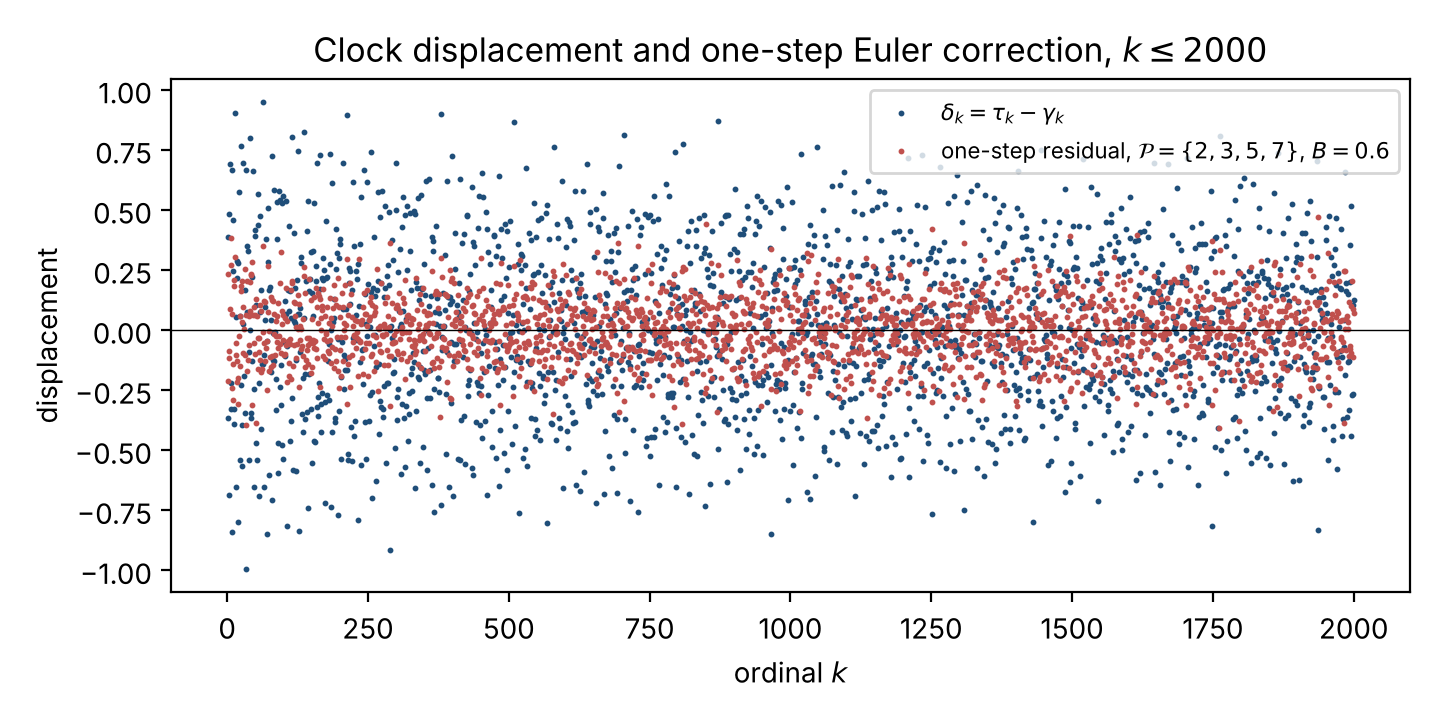
\includegraphics[width=0.86\textwidth]{fig01_displacement_first2000.png}
\caption{The displacement $\delta_k=\tau_k-\gamma_k$ of the RvM clock and the residual $\tau_k^{\PP}-\gamma_k$ of the one-step clock with $\PP=\{2,3,5,7\}$ and saturation $B=0.6$, for $k\le2000$.}
\label{fig:displacement}
\end{figure}

\subsection{Direct defects (Theorem B)}
\label{subsec:direct_defects}
For $T\in\{2^{14},2^{16},2^{18},2^{19}\}$ and $c\in\{\frac1{10},\frac15,\frac13,\frac12\}$ we compute $u_k(X)$ at the true ordinates with $X=T^c$ constant on $(T,2T]$; the windows contain $21\,519$, $100\,536$, $459\,982$ and $977\,804$ ordinates. Smaller exponents give $X<2$ at these heights and are excluded, as in Theorem~\CGref{thm:main}.

\begin{table}[htbp]
\centering\small
\caption{Mean squares of the defect $u_k(X)$ and of the one-step residual $r_k(X)$ over $T<\gamma_k\le2T$, $X=T^c$.}
\label{tab:direct}
\begin{tabular}{rrrrrrr}
\toprule
$T$ & $c$ & $X$ & $\#\{p\le X\}$ & $\langle u_k(X)^2\rangle$ & $\langle r_k(X)^2\rangle$ & $\frac1{2\pi^2}\log\frac1c$\\
\midrule
$2^{14}$ & $1/10$ & 2.64 & 1 & 0.066738 & 0.066312 & 0.116650\\
$2^{14}$ & $1/5$ & 6.96 & 3 & 0.039487 & 0.038425 & 0.081535\\
$2^{14}$ & $1/3$ & 25.40 & 9 & 0.020174 & 0.018347 & 0.055656\\
$2^{14}$ & $1/2$ & 128.00 & 31 & 0.010929 & 0.010701 & 0.035115\\
$2^{16}$ & $1/10$ & 3.03 & 2 & 0.056337 & 0.055961 & 0.116650\\
$2^{16}$ & $1/5$ & 9.19 & 4 & 0.039588 & 0.039045 & 0.081535\\
$2^{16}$ & $1/3$ & 40.32 & 12 & 0.022282 & 0.021508 & 0.055656\\
$2^{16}$ & $1/2$ & 256.00 & 54 & 0.011533 & 0.012316 & 0.035115\\
$2^{18}$ & $1/10$ & 3.48 & 2 & 0.062696 & 0.062544 & 0.116650\\
$2^{18}$ & $1/5$ & 12.13 & 5 & 0.041377 & 0.041265 & 0.081535\\
$2^{18}$ & $1/3$ & 64.00 & 18 & 0.022737 & 0.022855 & 0.055656\\
$2^{18}$ & $1/2$ & 512.00 & 97 & 0.011983 & 0.013848 & 0.035115\\
$2^{19}$ & $1/10$ & 3.73 & 2 & 0.065599 & 0.065517 & 0.116650\\
$2^{19}$ & $1/5$ & 13.93 & 6 & 0.040530 & 0.040623 & 0.081535\\
$2^{19}$ & $1/3$ & 80.63 & 22 & 0.022911 & 0.023446 & 0.055656\\
$2^{19}$ & $1/2$ & 724.08 & 128 & 0.012187 & 0.014567 & 0.035115\\
\bottomrule
\end{tabular}
\end{table}

\begin{figure}[htbp]
\centering
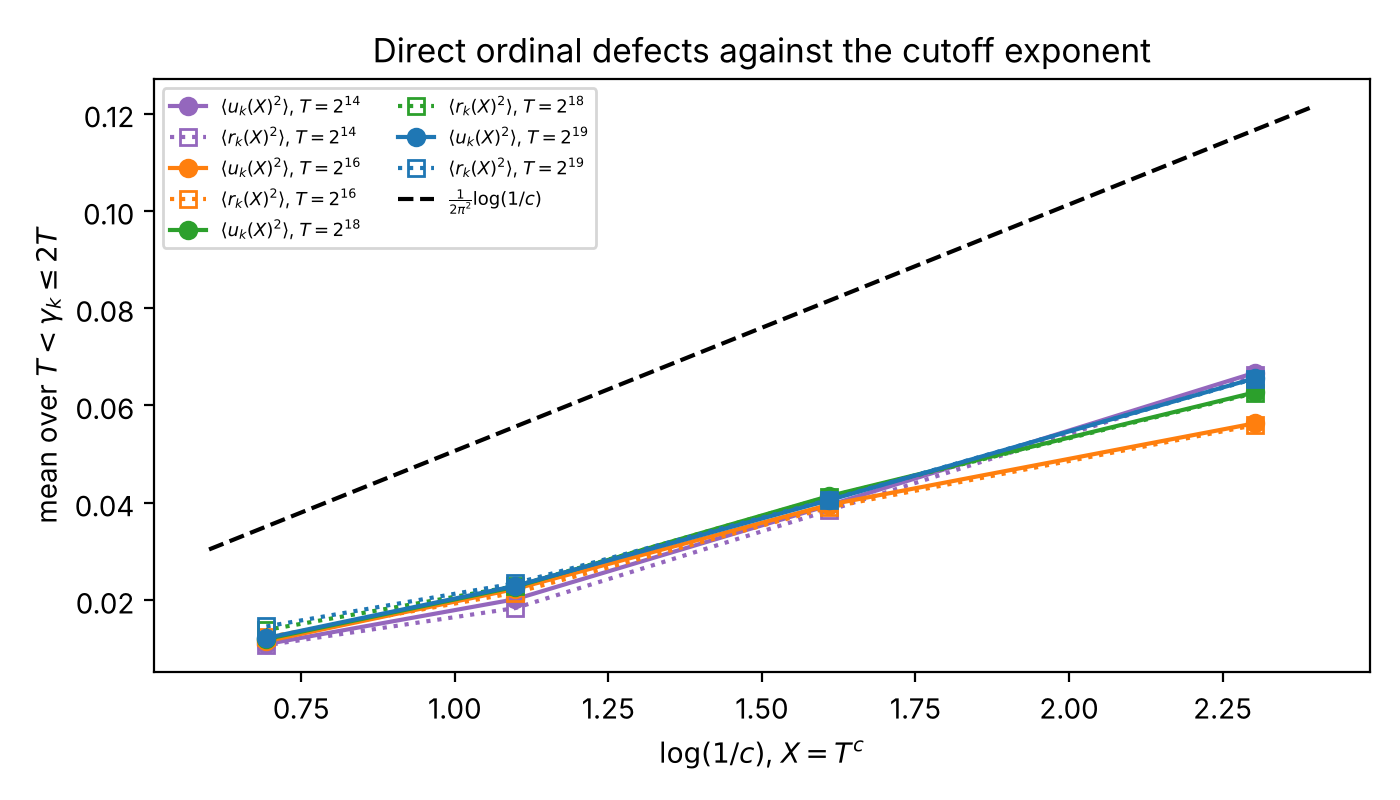
\includegraphics[width=0.86\textwidth]{fig02_direct_defects.png}
\caption{Mean square of $u_k(X)$ (filled markers) and of $r_k(X)$ (open markers) over $T<\gamma_k\le2T$ against $\log(1/c)$, $X=T^c$, for the four heights of Table~\CGref{tab:direct}; dashed: $\frac1{2\pi^2}\log(1/c)$.}
\label{fig:direct_defects}
\end{figure}

At fixed $c$ the measured means are essentially independent of $T$, as Theorem~\CGref{thm:main} requires of a bounded quantity, and they decrease monotonically in $c$. Between $c=\frac12$ and $c=\frac1{10}$ the increase of $\langle u_k^2\rangle$ at $T=2^{19}$ is $0.0534$, against $0.0815$ for the main term; at these heights the error term $O(1+\sqrt{\log(1/c)})$ is not small compared with the main term, and the data do not determine a limit at fixed $c$. The one-step residual $r_k(X)$ agrees with $u_k(X)$ to within $3\%$ for $c\le\frac15$ and exceeds it at $c=\frac12$ ($0.0146$ against $0.0122$ at $T=2^{19}$): this is the cost of evaluating $S_X$ at $\tau_k$ instead of $\gamma_k$ (Theorem~\CGref{thm:accounting}(a)).

\subsection{Exact accounting (Theorem C)}
\label{subsec:accounting_data}
For $X\in\{7,61,401,907,1999\}$ and the five windows above $k=1000$ we compute the gain $\langle s_k^2-(s_k-S_X(\tau_k))^2\rangle$, the diagonal term $D_X$ and the cross term $\Cr_X$ of \CGeqref{eq:full_factor_gain}. Table~\CGref{tab:accounting} lists three windows; Figure~\CGref{fig:accounting} shows all five.

\begin{table}[htbp]
\centering\small
\caption{Exact decomposition \CGeqref{eq:full_factor_gain} of the one-step gain into the diagonal term $D_X$ and the cross term $\Cr_X$.}
\label{tab:accounting}
\begin{tabular}{lrrrrrr}
\toprule
window of $k$ & $\langle s_k^2\rangle$ & $X$ & gain & $D_X$ & $\Cr_X$ & $v_X$\\
\midrule
$(10^3,10^4]$ & 0.085195 & 7 & 0.063224 & 0.063984 & 0.000760 & 0.066252\\
 &  & 61 & 0.075868 & 0.085258 & 0.009390 & 0.093853\\
 &  & 401 & 0.067945 & 0.097561 & 0.029616 & 0.111486\\
 &  & 907 & 0.062337 & 0.100483 & 0.038146 & 0.117730\\
 &  & 1999 & 0.055885 & 0.101829 & 0.045944 & 0.123202\\
\addlinespace
$(10^5,5\cdot10^5]$ & 0.106325 & 7 & 0.064185 & 0.064201 & 0.000016 & 0.066252\\
 &  & 61 & 0.086367 & 0.086579 & 0.000212 & 0.093853\\
 &  & 401 & 0.093276 & 0.096932 & 0.003657 & 0.111486\\
 &  & 907 & 0.092779 & 0.099690 & 0.006911 & 0.117730\\
 &  & 1999 & 0.091379 & 0.101921 & 0.010542 & 0.123202\\
\addlinespace
$(10^6,K]$ & 0.113224 & 7 & 0.064441 & 0.064444 & 0.000003 & 0.066252\\
 &  & 61 & 0.087434 & 0.087478 & 0.000044 & 0.093853\\
 &  & 401 & 0.098011 & 0.098495 & 0.000483 & 0.111486\\
 &  & 907 & 0.098607 & 0.101389 & 0.002782 & 0.117730\\
 &  & 1999 & 0.098325 & 0.103474 & 0.005149 & 0.123202\\
\bottomrule
\end{tabular}
\end{table}

\begin{figure}[htbp]
\centering
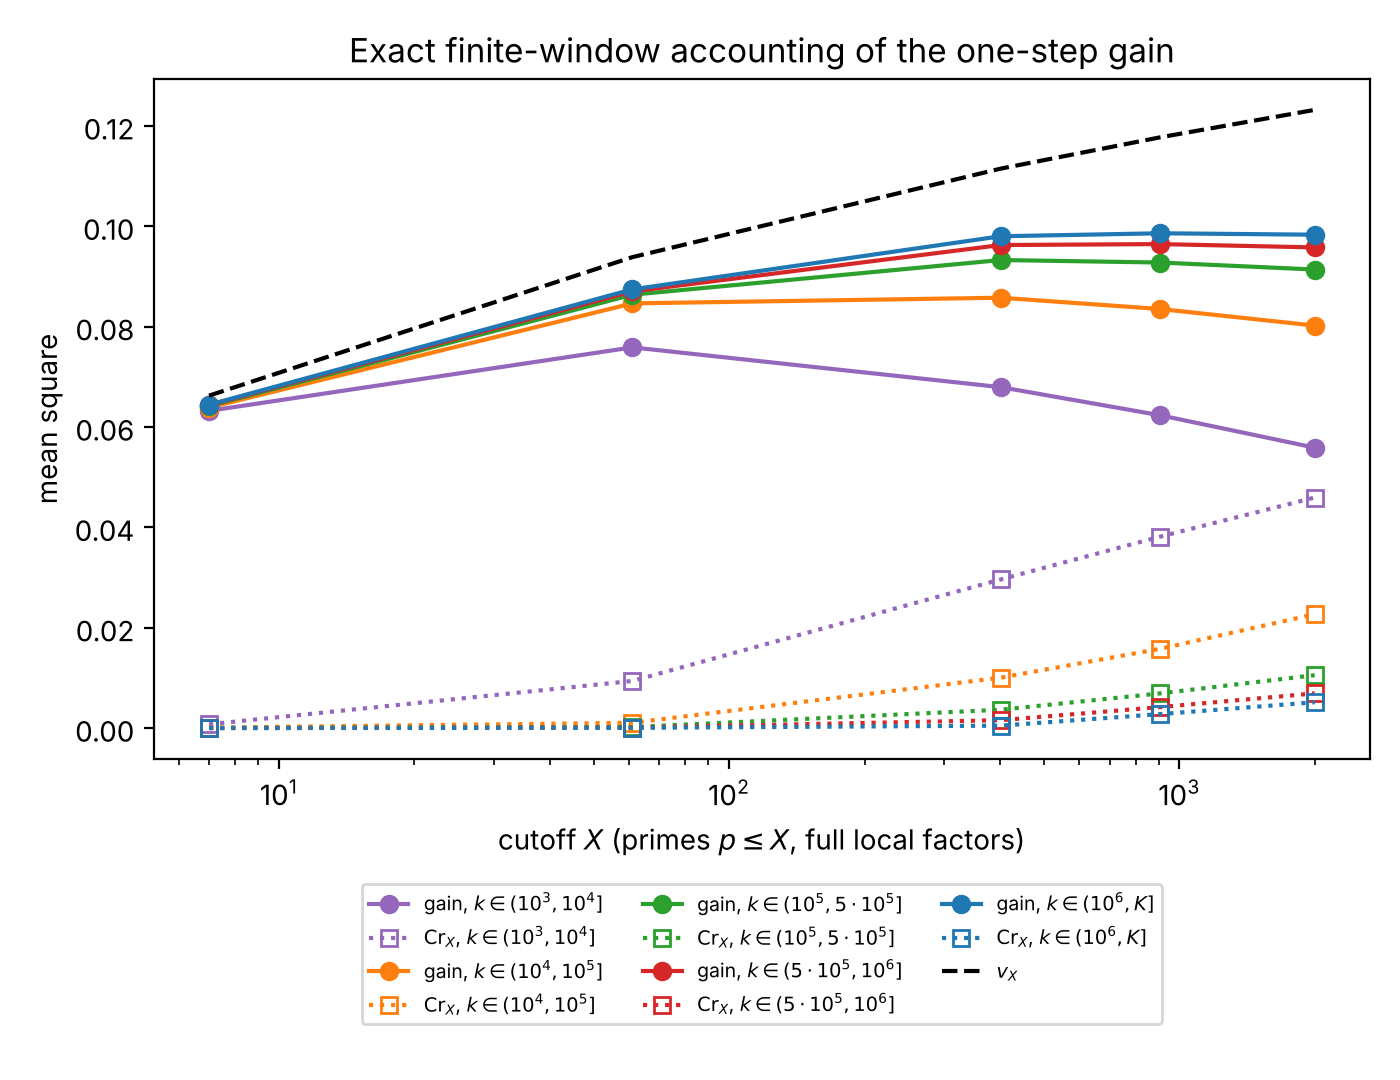
\includegraphics[width=0.86\textwidth]{fig03_accounting.png}
\caption{Gain of the one-step clock (filled markers) and cross term $\Cr_X$ (open markers) against the cutoff $X$, for five windows of ordinals; dashed: $v_X$.}
\label{fig:accounting}
\end{figure}

The diagonal term $D_X$ increases with $X$ in every window and stays below $v_X$; the cross term $\Cr_X$ grows with $X$ at fixed height and decreases with the height at fixed $X$. The gain is therefore maximal at a cutoff that increases with the height: $X=61$ on $(10^3,10^4]$, between $401$ and $1999$ on $(10^5,5\cdot10^5]$, and near $907$ on $(10^6,K]$. No parameter is fitted, and the identity gain $=D_X-\Cr_X$ is exact.

\subsection{The one-step clock against the cutoff}
\label{subsec:one_step_cutoff}
For comparison with \cite{FrancaLeClair2014,LeClair2021} we also report the root mean square and the maximum of $\tau_k^X-\gamma_k$ for $40$ cutoffs $2\le X\le1999$ (Figure~\CGref{fig:rms_cutoff}) and for five rules, with saturation $\tau_k-\sgn(y_k)\min(|y_k|,B)$, $y_k=S_X(\tau_k)/\lL(\tau_k)$, where indicated (Table~\CGref{tab:methods}, Figure~\CGref{fig:max_window}). The minimizing cutoff increases from $7$ on $(0,10^3]$ to $907$ on $(10^6,K]$, in agreement with the accounting above, and a least-squares fit $\log X_{\rm opt}=\theta_{\rm fit}\log(\tau/2\pi)$ over the five upper windows gives $\theta_{\rm fit}=0.5744$. This exponent is exploratory: the curves are flat near the minimum (in the top window the root mean square is $0.06447$ at $X=701$, $0.06427$ at $X=907$ and $0.06428$ at $X=1009$), and it is not asserted to be asymptotically optimal. A large fixed cutoff is harmful at small heights: $\PP=\{p\le1999\}$ gives the residual $3.247$ at $k=1$. The largest residual for $\PP=\{2,3,5,7\}$, at $k=258\,318$, follows the close pair $\gamma_{258317}=175\,681.6491$, $\gamma_{258318}=175\,681.7159$ (normalized gap $0.109$), at which $S(\gamma_{258318})=1.039$ and $\delta_{258318}=0.638$.

\begin{table}[htbp]
\centering\footnotesize
\caption{Root mean square, maximum of $|\tau_k^X-\gamma_k|$ and number of residuals $\ge\frac12$ over all $K$ ordinates, and the same quantities in the top window $(10^6,K]$.}
\label{tab:methods}
\setlength{\tabcolsep}{4pt}
\begin{tabular}{lrrrrrr}
\toprule
rule & RMS & max & $\#\ge\frac12$ & RMS, top & max, top & $\#\ge\frac12$, top\\
\midrule
bare clock $\tau_k$ & 0.188066 & 0.993711 & 11589 & 0.178900 & 0.717359 & 2971\\
$\mathcal P=\{2,3,5,7\}$, $B=0.6$ & 0.120691 & 0.522347 & 1 & 0.117413 & 0.489293 & 0\\
$\mathcal P=\{p\le61\}$, $B=0.6$ & 0.085635 & 0.457259 & 0 & 0.085354 & 0.400144 & 0\\
$\mathcal P=\{p\le1999\}$, no saturation & 0.070757 & 3.247397 & 156 & 0.064897 & 0.528267 & 7\\
$X_k=\max(7,(\tau_k/2\pi)^{0.57})$, $B=0.6$ & 0.066608 & 0.513886 & 2 & 0.064259 & 0.513886 & 1\\
\bottomrule
\end{tabular}
\end{table}

\begin{figure}[htbp]
\centering
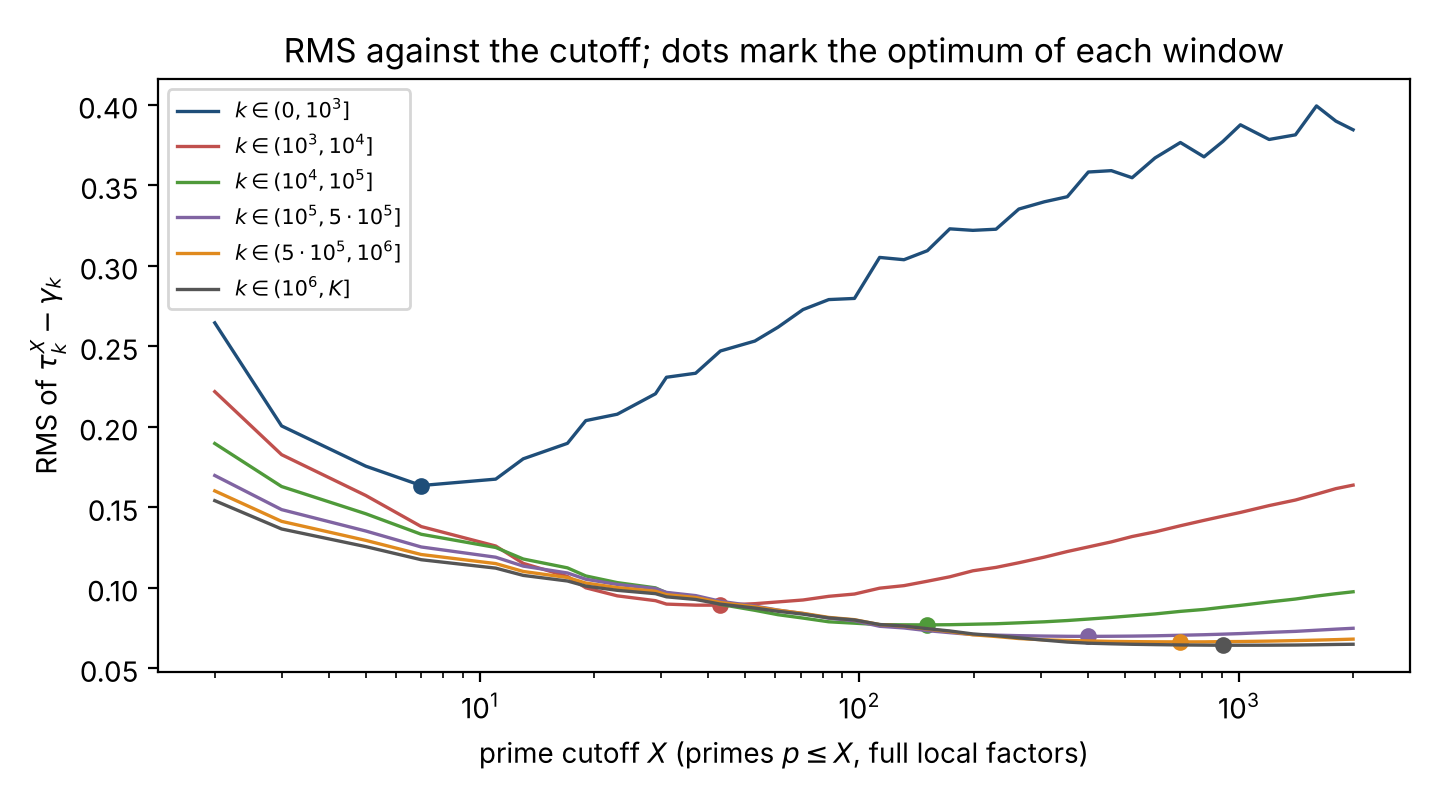
\includegraphics[width=0.86\textwidth]{fig04_rms_vs_cutoff.png}
\caption{Root mean square of $\tau_k^X-\gamma_k$ (no saturation) against the cutoff $X$, by window of ordinals; dots mark the minimum in each window.}
\label{fig:rms_cutoff}
\end{figure}

\begin{figure}[htbp]
\centering
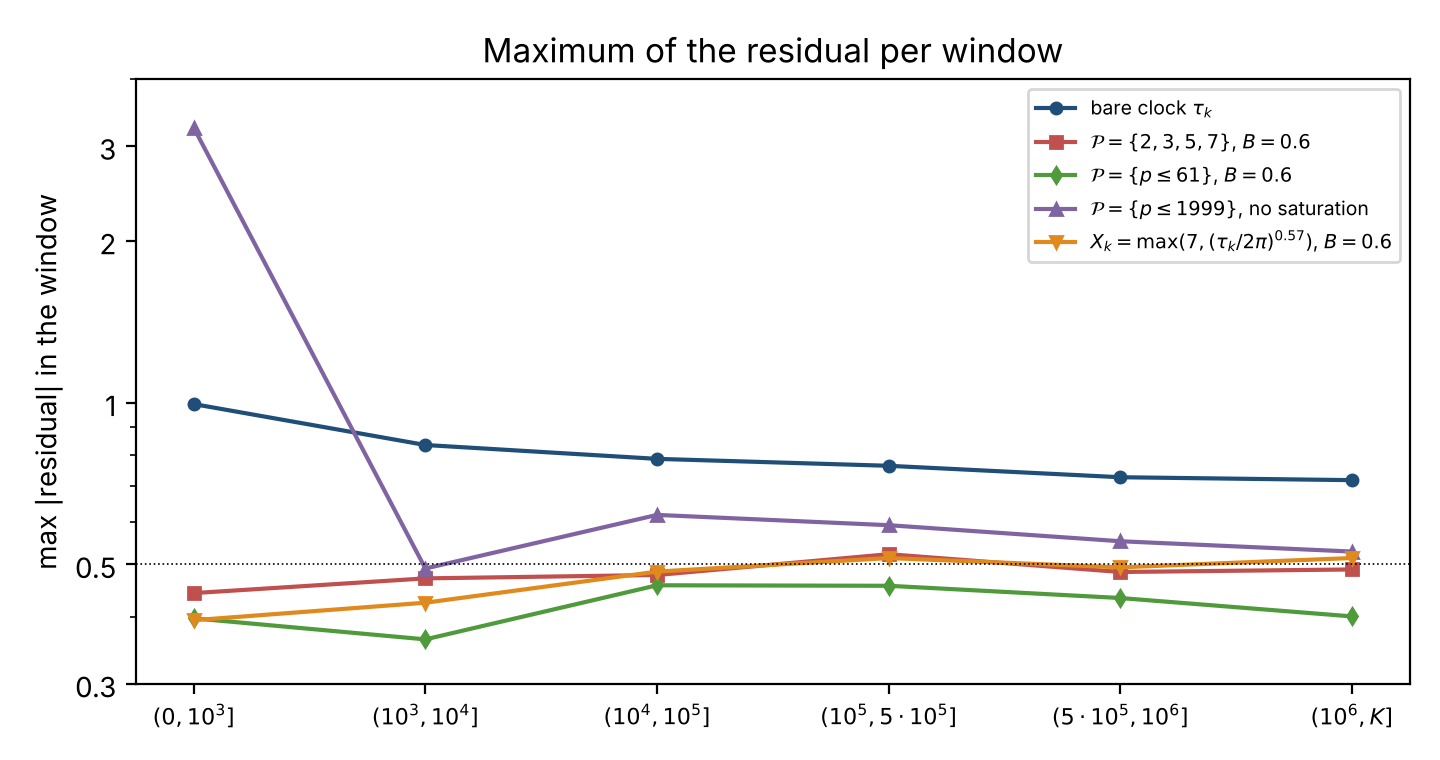
\includegraphics[width=0.86\textwidth]{fig05_max_by_window.png}
\caption{Maximum of $|\tau_k^X-\gamma_k|$ in each window of ordinals for the five rules of Table~\CGref{tab:methods}; dotted: $\frac12$.}
\label{fig:max_window}
\end{figure}

%======================================================================
\section{Conditional results}
\label{sec:conditional}

\emph{Every statement of this section is either an unconditional identity or a rigorous implication from a named hypothesis. Nothing heuristic is used, and Theorems~\CGref{thm:identity_general}, \CGref{thm:main} and \CGref{thm:accounting} do not depend on this section.}

\subsection{Fixed frequencies under Hypothesis L}
\label{subsec:hypL}

\begin{hypothesis}[Hypothesis L: fixed-frequency Landau formula on the critical line]\label{hyp:L}
For every fixed integer $n\ge2$, $\sum_{0<\gamma\le t}n^{i\gamma}=-\frac t{2\pi}\frac{\Lambda(n)}{\sqrt n}+o(t)$, the zeros of the Riemann zeta function being counted with multiplicity.
\end{hypothesis}

\begin{proposition}\label{prop:L_sufficient}
Hypothesis~L holds if $\sum_{0<\gamma\le t}|\beta-\frac12|=o(t)$.
\end{proposition}

\begin{proof}
$|n^\rho-\sqrt n\,n^{i\gamma}|=|n^\beta-n^{1/2}|\le n\log n\,|\beta-\frac12|$ by the mean value theorem, since $0<\beta<1$; apply Theorem~\CGref{thm:known_landau}.
\end{proof}

\begin{lemma}\label{lem:clock_equidistribution}
For fixed real $\omega\ne0$, $\sum_{k\in\IT}e^{i\omega\tau_k}\ll_\omega\log T$. Hence for fixed integers $n_1,n_2\ge2$, $\langle\sin(\tau_k\log n_1)\sin(\tau_k\log n_2)\rangle_{\IT}\to\frac12\mathbf 1_{n_1=n_2}$.
\end{lemma}

\begin{proof}
Take $\omega>0$ (conjugate otherwise) and $\Omega(x)=\omega\tau_x/2\pi$ for real $x\ge1$. By \CGeqref{eq:clock}, $\Omega'(x)=\omega/\log(\tau_x/2\pi)$ is continuous, positive and decreasing, and for $x\in[\min\IT,\max\IT]$ and $T\ge T_0(\omega)$ it lies in $[\omega/\log(T/\pi),\frac12]$, so that $\|\Omega'\|\ge\omega/\log(T/\pi)$. $\IT$ is a set of consecutive integers, and Theorem~\CGref{thm:known_KL} gives the bound. For the second claim use $2\sin y_1\sin y_2=\cos(y_1-y_2)-\cos(y_1+y_2)$ with $\omega=\log(n_1/n_2)$ (if $n_1\ne n_2$) and $\omega=\log(n_1n_2)$, and $\#\IT\asymp T\log T$.
\end{proof}

\begin{theorem}[Under Hypothesis L]\label{thm:projection}
Assume Hypothesis~L. For every fixed integer $n\ge2$, $\langle s_k\sin(\gamma_k\log n)\rangle_{\IT}\to\frac{a_n}2$, and the same with $\tau_k$ in place of $\gamma_k$; thus $\Rg_n(\IT),\Rt_n(\IT)\to1$ for prime powers $n$.
\end{theorem}

\begin{proof}
For $t>14$ not an ordinate let $\mathcal H_n(t)=\int_{14}^tS(y)n^{iy}dy$; the integrand is bounded and piecewise continuous. As measures on $(14,t]$, $dS=dN-(\lL+\varpi'/\pi)dy$, and $y\mapsto n^{iy}/(i\ell_n)$ is a $C^1$ primitive of $n^{iy}$; integration by parts for Lebesgue--Stieltjes integrals gives
\begin{equation}
\mathcal H_n(t)=\Bigl[\frac{S(y)n^{iy}}{i\ell_n}\Bigr]_{14}^t-\frac1{i\ell_n}\sum_{14<\gamma_k\le t}n^{i\gamma_k}+\frac1{i\ell_n}\int_{14}^tn^{iy}\Bigl(\lL+\frac{\varpi'}\pi\Bigr)dy=\frac i{\ell_n}\sum_{0<\gamma_k\le t}n^{i\gamma_k}+O(\log t),
\label{eq:projection_Phi}
\end{equation}
since $\gamma_1>14$, $S=O(\log t)$, $\int_{14}^tn^{iy}\lL\,dy=O(\log t)$ by a second integration by parts ($\lL'(y)=1/(2\pi y)$), and $\varpi'=O(y^{-2})$. Hypothesis~L gives $\mathcal H_n(t)=-i\frac{\Lambda(n)}{2\pi\sqrt n\,\ell_n}t+o(t)$. Integrating by parts once more, with $\frac d{dt}(t\lL(t))=\lL(t)+\frac1{2\pi}$,
\begin{equation}
\int_T^{2T}S(t)n^{it}\lL(t)\,dt=\bigl[\mathcal H_n\lL\bigr]_T^{2T}-\int_T^{2T}\frac{\mathcal H_n(t)}{2\pi t}\,dt=-i\frac{\Lambda(n)}{2\pi\sqrt n\,\ell_n}\int_T^{2T}\lL\,dt+o(T\log T).
\label{eq:projection_partial}
\end{equation}
Taking imaginary parts, $\int_T^{2T}S\sin(\ell_nt)\lL\,dt=\frac{a_n}2\int_T^{2T}\lL\,dt+o(T\log T)$. Apply Lemma~\CGref{lem:first_moment_identity} with $\psi(t)=\sin(\ell_nt)$ on $[t_1,t_2]$, where $t_1\in[T,T+1/T]$ and $t_2\in[2T,2T+1/T]$ are non-ordinates; the change of endpoints alters both sides by $O(\log^2T)$. The $\varpi$-term is $O(\log T)$, the boundary term is $O(\log^2T)$, and $\frac12\int G^2|\psi'|\ll\int_T^{2T}S^2+O(1)\ll T\log\log T$ by Theorem~\CGref{thm:known_selberg_moments}. Divide by $\#\IT=\int_T^{2T}\lL\,dt+O(\log T)$. For $\tau_k$: $|\sin(\ell_n\tau_k)-\sin(\ell_n\gamma_k)|\le\ell_n|\delta_k|$, and by \CGeqref{eq:s_delta} and Remark~\CGref{rem:korolev}, $\sum_{k\in\IT}|s_k\delta_k|\ll(\log T)^{-1}\sum_{k\in\IT}s_k^2\ll\#\IT\log\log T/\log T$.
\end{proof}

\begin{corollary}[Under Hypothesis L]\label{cor:gain}
For a finite set $A$ of prime powers and $\lambda\in\R$, $\langle s_k^2-(s_k-\lambda S_A(\tau_k))^2\rangle_{\IT}\to(2\lambda-\lambda^2)v_A$, maximal at $\lambda=1$.
\end{corollary}

\begin{proof}
In \CGeqref{eq:exact_gain}, $\Rt_n(\IT)\to1$ by Theorem~\CGref{thm:projection} and $\Cr_A(\IT)\to0$ by Lemma~\CGref{lem:clock_equidistribution}.
\end{proof}

The passage to the full local factors inside the limit needs uniformity in $n$, which is not proved. Figure~\CGref{fig:gain_fixed} shows the gains of two fixed prime sets approaching $v_\PP$ from below as the height increases.

\begin{figure}[htbp]
\centering
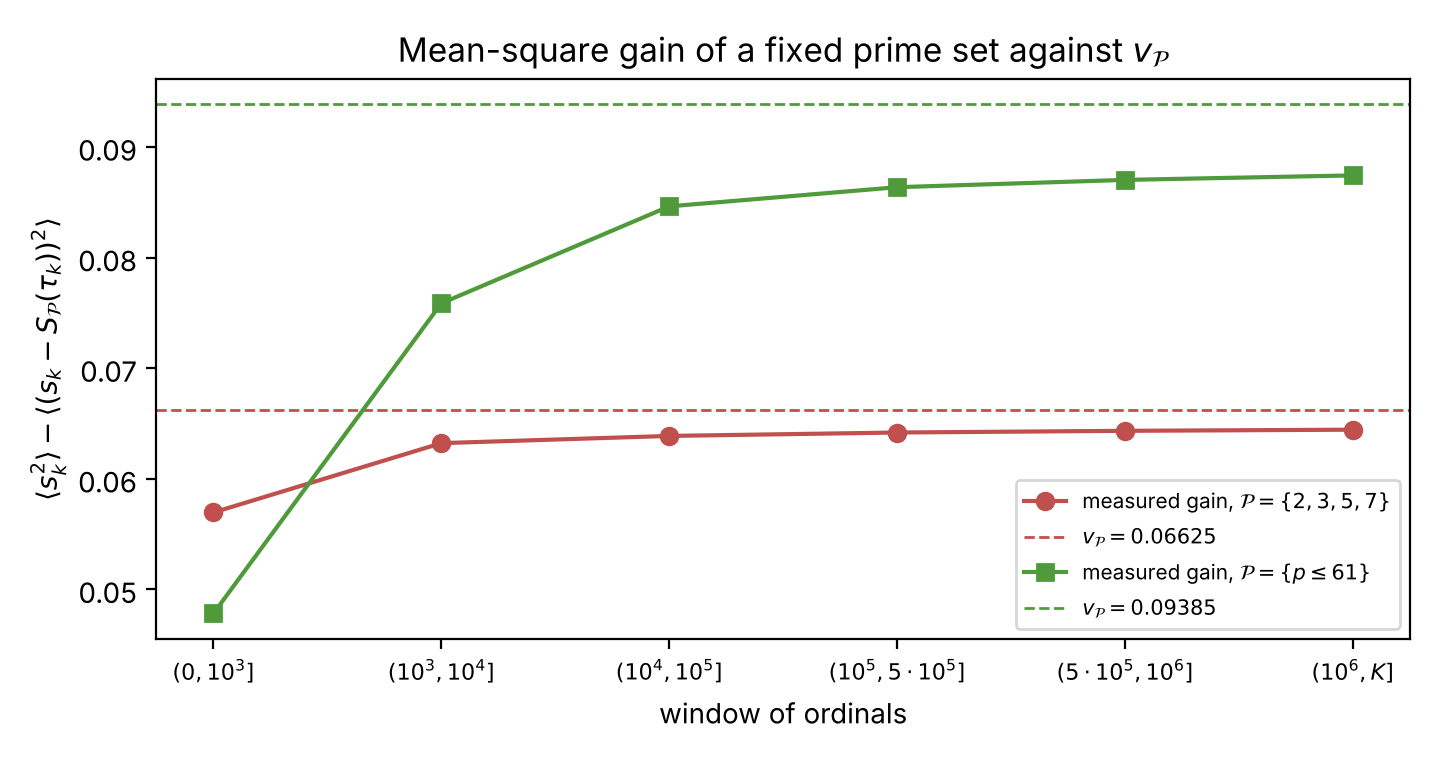
\includegraphics[width=0.86\textwidth]{fig06_gain_fixed_sets.png}
\caption{Mean-square gain $\langle s_k^2\rangle-\langle(s_k-S_\PP(\tau_k))^2\rangle$ of two fixed prime sets $\PP$ (full local factors) in each window of ordinals, and the constants $v_\PP$ (dashed) of Corollary~\CGref{cor:gain}.}
\label{fig:gain_fixed}
\end{figure}

\subsection{The response at the ordinates and its Fourier reduction}
\label{subsec:gamma_response}
Let $T,2T$ be non-ordinates, $p$ a prime, and
\begin{equation}
\mathcal A_{T,p}=-\frac{2\pi\sqrt p}{\#\IT}\int_T^{2T}G(t)\sin(t\log p)\lL(t)\,dt,
\qquad \mathcal S_{T,p}=\frac1T\int_T^{2T}S(t)^2p^{it}\,dt.
\label{eq:ATp_STp}
\end{equation}

\begin{proposition}[Unconditional separation of one- and two-point terms]\label{prop:gamma_response_exact}
\begin{equation}
\begin{split}
\Rg_p(\IT)={}&\mathcal A_{T,p}+\frac{\pi\sqrt p\,T\log p}{\#\IT}\Re\mathcal S_{T,p}-\frac{\pi\sqrt p}{\#\IT}\bigl[G^2\sin(t\log p)\bigr]_T^{2T}\\
&+\frac{\pi\sqrt p\log p}{\#\IT}\int_T^{2T}(G^2-S^2)\cos(t\log p)\,dt.
\end{split}
\label{eq:gamma_response_exact}
\end{equation}
If $\theta=\log p/L_T$ stays in a compact subset of $(0,1)$, the last two terms are $o(1)$ and
\begin{equation}
\Rg_p(\IT)=\mathcal A_{T,p}+2\pi^2\theta\sqrt p\,\bigl(1+O(1/L_T)\bigr)\Re\mathcal S_{T,p}+o(1).
\label{eq:gamma_response_scaled}
\end{equation}
\end{proposition}

\begin{proof}
Lemma~\CGref{lem:first_moment_identity} with $\psi(t)=\sin(t\log p)$ on $[T,2T]$, multiplied by $-2\pi\sqrt p/\#\IT$, gives \CGeqref{eq:gamma_response_exact}, because $\int_T^{2T}G^2\cos(t\log p)\,dt=T\Re\mathcal S_{T,p}+\int_T^{2T}(G^2-S^2)\cos(t\log p)\,dt$. On $[T,2T]$, $|G^2-S^2|\le2|S||\varpi|/\pi+\varpi^2/\pi^2\ll\log T/T$, so the last term is $O(\sqrt p\log p/T)$, and the boundary term is $O(\sqrt p\log^2T/(T\log T))$. Both are $o(1)$ for $p\le T^{\theta_1}$ with $\theta_1<1$. Finally $\#\IT=\frac{TL_T}{2\pi}(1+O(1/L_T))$.
\end{proof}

Let $f_T=S\mathbf1_{[T,2T]}$, let $\mathfrak m_T$ be its distributional derivative (a finite signed measure, since $f_T$ has compact support and bounded variation), and
\begin{equation}
Z_T(\omega)=\int_\R e^{i\omega t}\,d\mathfrak m_T(t),\qquad \widehat{f_T}(\omega)=\int_\R f_T(t)e^{i\omega t}dt .
\label{eq:measure_def}
\end{equation}

\begin{theorem}[Unconditional shifted two-point representation]\label{thm:Fourier_exact}
For non-ordinates $T,2T$,
\begin{equation}
Z_T(\omega)=\sum_{T<\gamma<2T}\nu(\gamma)e^{i\omega\gamma}-\int_T^{2T}\Bigl(\lL(t)+\frac{\varpi'(t)}\pi\Bigr)e^{i\omega t}\,dt+S(T)e^{i\omega T}-S(2T)e^{2i\omega T},
\label{eq:measure_expansion}
\end{equation}
$Z_T(\omega)=-i\omega\widehat{f_T}(\omega)$, so that $Z_T(0)=0$ and $Z_T(\omega)/\omega$ extends continuously by $-i\widehat{f_T}$; and for every real $\omega_0$
\begin{equation}
\int_T^{2T}S(t)^2e^{i\omega_0t}\,dt=-\frac1{2\pi}\int_\R\frac{Z_T(\omega)Z_T(\omega_0-\omega)}{\omega(\omega_0-\omega)}\,d\omega,
\label{eq:Fourier_convolution}
\end{equation}
the integral converging absolutely.
\end{theorem}

\begin{proof}
On $(T,2T)$, $dS=dN-(\lL+\varpi'/\pi)dt$ as measures, with atoms $\nu(\gamma)\delta_\gamma$; the cutoff adds $S(T)\delta_T$ and $-S(2T)\delta_{2T}$. This gives $\mathfrak m_T$ and \CGeqref{eq:measure_expansion}. Since $f_T$ is of bounded variation with compact support, integration by parts gives $\int e^{i\omega t}d\mathfrak m_T=-i\omega\int f_Te^{i\omega t}dt$, the boundary terms vanishing. As $f_T\in L^1\cap L^2$ is real, Plancherel's identity applied to $f_T$ and $f_Te^{-i\omega_0t}$ gives $\int f_T^2e^{i\omega_0t}dt=\frac1{2\pi}\int\widehat{f_T}(\omega)\widehat{f_T}(\omega_0-\omega)\,d\omega$, absolutely convergent since $\int|\widehat{f_T}(\omega)\widehat{f_T}(\omega_0-\omega)|d\omega\le\|\widehat{f_T}\|_2^2=2\pi\|f_T\|_2^2$. Substitute $\widehat{f_T}=iZ_T/\omega$.
\end{proof}

With $\omega_0=\theta L_T=\log p$ and $\omega=\alpha L_T$ put
\begin{equation}
\mathcal B_T(\theta)=\int_\R\frac{Z_T(\alpha L_T)Z_T((\theta-\alpha)L_T)}{\alpha(\theta-\alpha)}\,d\alpha,\qquad\text{so that}\qquad \mathcal S_{T,p}=-\frac{\mathcal B_T(\theta)}{2\pi TL_T}.
\label{eq:BT_scaled}
\end{equation}
Expanding the zero sums gives the weights $e^{i\alpha L_T\gamma}e^{i(\theta-\alpha)L_T\gamma'}=p^{i\gamma'}e^{i\alpha L_T(\gamma-\gamma')}$: $\mathcal S_{T,p}$ is a pair correlation of the zeros of the Riemann zeta function \emph{shifted by a prime frequency}, which a stationary pair correlation (a function of $\gamma-\gamma'$ only) does not determine.

\subsection{The kernel $\mathfrak K_\theta$}
\label{subsec:kernel}
For $0<\theta<1$ define the continuous, piecewise linear function
\begin{equation}
\mathfrak K_\theta(\alpha)=
\begin{cases}
\theta,&\alpha\le-1,\\
\theta-1-\alpha,&-1\le\alpha\le\theta-1,\\
0,&\theta-1\le\alpha\le1,\\
\alpha-1,&1\le\alpha\le1+\theta,\\
\theta,&\alpha\ge1+\theta,
\end{cases}
\label{eq:kernel_piecewise}
\end{equation}
equivalently, with $h(q)=\max(1-|q|,0)$,
\begin{equation}
\mathfrak K_\theta(\alpha)=1-h(\alpha)-h(\theta-\alpha)-h(\theta)+2\max\bigl(1-\max(|\alpha|,|\theta-\alpha|,\theta),0\bigr),
\label{eq:kernel_intersections}
\end{equation}
as one checks on each of the five intervals.

\begin{proposition}[Integral and support of the kernel]\label{prop:kernel_integral}
For $0<\theta<1$,
\begin{equation}
\int_\R\frac{\mathfrak K_\theta(\alpha)}{\alpha(\theta-\alpha)}\,d\alpha=-\frac{2\Phi(\theta)}{\theta},
\label{eq:kernel_integral}
\end{equation}
the integral being absolutely convergent, and $\mathfrak K_\theta(\alpha)=0$ whenever $|\alpha|+|\theta-\alpha|+\theta<2$.
\end{proposition}

\begin{proof}
$\mathfrak K_\theta$ is bounded and vanishes on $[\theta-1,1]$, which contains $0$ and $\theta$; the integrand is bounded, continuous outside $[\theta-1,1]$ and $O(\alpha^{-2})$ as $|\alpha|\to\infty$, hence absolutely integrable. It is invariant under $\alpha\mapsto\theta-\alpha$, which maps $[1,\infty)$ onto $(-\infty,\theta-1]$, so the integral is twice that over $[1,\infty)$. On $[1+\theta,\infty)$, $\frac{\theta}{\alpha(\theta-\alpha)}=\frac1\alpha-\frac1{\alpha-\theta}$, whose integral is $\lim_{y\to\infty}\bigl[\log\frac{\alpha}{\alpha-\theta}\bigr]_{1+\theta}^{y}=-\log(1+\theta)$. On $[1,1+\theta]$, $\frac{\alpha-1}{\alpha(\theta-\alpha)}=-\frac1{\theta\alpha}+\frac{\theta-1}{\theta(\theta-\alpha)}$, whose integral is $-\frac{\log(1+\theta)}\theta+\frac{\theta-1}\theta\log(1-\theta)$. The sum is $-\Phi(\theta)/\theta$; doubling gives \CGeqref{eq:kernel_integral}. If $\alpha>1$ then $|\alpha|+|\theta-\alpha|+\theta\ge\alpha+(\alpha-\theta)+\theta=2\alpha>2$, and if $\alpha<\theta-1$ the same follows by the symmetry; elsewhere $\mathfrak K_\theta=0$.
\end{proof}

\subsection{The moving-prime law under Hypotheses U and W}
\label{subsec:conditional_law}

\begin{hypothesis}[Hypothesis U: uniform one-particle input]\label{hyp:uniform_prime}
For every $0<\theta_0<\theta_1<1$, uniformly for primes with $\theta_0\le\log p/L_T\le\theta_1$, $\mathcal A_{T,p}=1+o(1)$.
\end{hypothesis}
A sufficient condition is the uniform estimate $\sup_{T\le t\le2T}|\sum_{T<\gamma_k\le t}p^{i\gamma_k}+\frac{(t-T)\log p}{2\pi\sqrt p}|=o(T\log p/\sqrt p)$ in that range, by two integrations by parts as in the proof of Theorem~\CGref{thm:projection}. Theorem~\CGref{thm:known_landau} concerns fixed bases and $p^\rho$, and does not give it.

\begin{hypothesis}[Hypothesis W: weighted arithmetic bridge]\label{hyp:weighted_bridge}
Uniformly for primes with $\theta$ in any compact subset of $(0,1)$,
\begin{equation}
\int_\R\frac{Z_T(\alpha L_T)Z_T((\theta-\alpha)L_T)+\mathcal N_Tp^{-1/2}\mathfrak K_\theta(\alpha)}{\alpha(\theta-\alpha)}\,d\alpha=o\Bigl(\frac{TL_T}{\sqrt p}\Bigr),
\label{eq:weighted_arithmetic_bridge}
\end{equation}
with the continuous extensions of $Z_T(\omega)/\omega$ at $\omega=0$.
\end{hypothesis}

\begin{proposition}[Moving-prime law under Hypotheses U and W]\label{prop:conditional_universal}
Under Hypothesis~W,
\begin{equation}
\mathcal S_{T,p}=-\frac{1}{2\pi^2\sqrt p}\frac{\Phi(\theta)}{\theta}+o(p^{-1/2}).
\label{eq:CTp_target}
\end{equation}
Under Hypotheses~U and W, or U and the real part of \CGeqref{eq:CTp_target}, uniformly for $\theta$ in compact subsets of $(0,1)$,
\begin{equation}
\Rg_p(\IT)=1-\Phi(\theta)+o(1).
\label{eq:conditional_universal}
\end{equation}
Conversely, under Hypothesis~U, \CGeqref{eq:conditional_universal} is equivalent to the real part of \CGeqref{eq:CTp_target}. Nothing is asserted about $\Rt_p$.
\end{proposition}

\begin{proof}
The integral of the kernel term in \CGeqref{eq:weighted_arithmetic_bridge} converges absolutely (Proposition~\CGref{prop:kernel_integral}); hence so does that of the first term, which is $\mathcal B_T(\theta)$, and by \CGeqref{eq:kernel_integral} $\mathcal B_T(\theta)=\frac{\mathcal N_T}{\sqrt p}\frac{2\Phi(\theta)}\theta+o(TL_T/\sqrt p)=\frac{TL_T}{\pi\sqrt p}\frac{\Phi(\theta)}\theta+o(TL_T/\sqrt p)$; \CGeqref{eq:BT_scaled} gives \CGeqref{eq:CTp_target}. Then $\sqrt p\,\Re\mathcal S_{T,p}=O(1)$, so in \CGeqref{eq:gamma_response_scaled} the factor $1+O(1/L_T)$ contributes $o(1)$ and $2\pi^2\theta\sqrt p\,\Re\mathcal S_{T,p}=-\Phi(\theta)+o(1)$; with $\mathcal A_{T,p}=1+o(1)$ this is \CGeqref{eq:conditional_universal}. Conversely, solve \CGeqref{eq:gamma_response_scaled} for $\Re\mathcal S_{T,p}$.
\end{proof}

\begin{remark}\label{rem:scale_gap}
$\Phi(\theta)=2\sum_{j\ge1}\frac{\theta^{2j}}{(2j-1)2j}=\theta^2+\frac{\theta^4}6+\frac{\theta^6}{15}+\cdots$, so $1-\theta^2$ is only the quadratic truncation of \CGeqref{eq:conditional_universal}, and $1-\Phi(\theta)$ vanishes at $\theta=0.9036\ldots$. Hypotheses U and W are not consequences of Hypothesis~L. The prime polynomial alone does not give \CGeqref{eq:CTp_target}: writing $S=S^{\rm pr}_Y+(S-S^{\rm pr}_Y)$, the square $(S^{\rm pr}_Y)^2$ has no exact Fourier frequency $\log p$, and Selberg's estimate gives only $|T^{-1}\int_T^{2T}(S-S^{\rm pr}_Y)^2p^{it}dt|\ll1$, whereas \CGeqref{eq:CTp_target} needs the error $o(p^{-1/2})=T^{-\theta/2+o(1)}$.
\end{remark}

%======================================================================
\section{Heuristic support and numerical evidence}
\label{sec:heuristic}

\emph{This section contains no statement about the Riemann zeta function that is used elsewhere. Subsection~\CGref{subsec:det_model} proves a theorem about a random-matrix model; its relevance to the zeros of the Riemann zeta function is a heuristic.}

\subsection{A determinantal model whose connected kernel is $\mathfrak K_\theta$}
\label{subsec:det_model}
On a circle of length $R_0$ let $\Pi_{\mathfrak n}$ be the orthogonal projection onto $\mathfrak n$ consecutive Fourier modes, and consider its determinantal point process, which has exactly $\mathfrak n$ points. For $q\in R_0^{-1}\mathbb Z$ let $\Xi_q$ be the centred linear statistic of $y\mapsto e^{2\pi iqy}$, so that $\Xi_0=0$ and $\overline{\Xi_q}=\Xi_{-q}$. Let $R_0,\mathfrak n\to\infty$ with $\mathfrak n/R_0\to1$, so that the local kernel tends to the sine kernel. For lattice $\theta>0$ and real $\iota_1,\iota_2$ the tilt
\begin{equation}
d\mathbb P_{\iota_1,\iota_2}=\frac{\exp\{-\iota_1\Re\Xi_{-\theta}-\iota_2\Im\Xi_{-\theta}\}}{\mathbb E\exp\{-\iota_1\Re\Xi_{-\theta}-\iota_2\Im\Xi_{-\theta}\}}\,d\mathbb P_{0,0}
\label{eq:real_tilt}
\end{equation}
is a probability measure (the statistics are bounded), and differentiation at $(0,0)$, justified by boundedness, gives $(\partial_{\iota_1}+i\partial_{\iota_2})\operatorname{Cov}_{\iota_1,\iota_2}(\Xi_\alpha,\Xi_{\theta-\alpha})|_{(0,0)}=-\operatorname{cum}_3(\Xi_\alpha,\Xi_{\theta-\alpha},\Xi_{-\theta})$, the third joint cumulant.

\begin{theorem}[Connected kernel of the model]\label{thm:sine_kernel}
Let lattice frequencies tend to $\alpha,\theta-\alpha,-\theta$ with $0<\theta<1$. Then $R_0^{-1}\operatorname{cum}_3(\Xi_\alpha,\Xi_{\theta-\alpha},\Xi_{-\theta})\to\mathfrak K_\theta(\alpha)$ and $R_0^{-1}\operatorname{cum}_2(\Xi_\theta,\Xi_{-\theta})\to\theta$.
\end{theorem}

\begin{proof}
For commuting multiplication operators $\mathsf m_1,\mathsf m_2,\mathsf m_3$, the third joint cumulant of the corresponding linear statistics of a determinantal process with projection kernel is \cite{Soshnikov2002}
\begin{equation}
\begin{split}
\operatorname{cum}_3={}&\operatorname{Tr}(\mathsf m_1\mathsf m_2\mathsf m_3\Pi_{\mathfrak n})-\operatorname{Tr}(\mathsf m_1\mathsf m_2\Pi_{\mathfrak n}\mathsf m_3\Pi_{\mathfrak n})-\operatorname{Tr}(\mathsf m_1\mathsf m_3\Pi_{\mathfrak n}\mathsf m_2\Pi_{\mathfrak n})-\operatorname{Tr}(\mathsf m_2\mathsf m_3\Pi_{\mathfrak n}\mathsf m_1\Pi_{\mathfrak n})\\
&+\operatorname{Tr}(\mathsf m_1\Pi_{\mathfrak n}\mathsf m_2\Pi_{\mathfrak n}\mathsf m_3\Pi_{\mathfrak n})+\operatorname{Tr}(\mathsf m_1\Pi_{\mathfrak n}\mathsf m_3\Pi_{\mathfrak n}\mathsf m_2\Pi_{\mathfrak n}),
\end{split}
\label{eq:third_cumulant_trace}
\end{equation}
the third-order term of the expansion of $\log\det(\mathrm{Id}+\Pi_{\mathfrak n}(e^{\mathsf m}-1)\Pi_{\mathfrak n})$. Multiplication by $e^{2\pi iqy}$ shifts a mode by $R_0q$; a trace with two projections counts the overlap of two integer intervals of length $\mathfrak n$, and a trace with three their triple overlap. For the shifts $R_0\alpha$, $R_0(\theta-\alpha)$, $-R_0\theta$, whose sum is $0$, the triple overlap has length $\max(\mathfrak n-R_0\max(|\alpha|,|\theta-\alpha|,\theta),0)$ for both cyclic orders, and the pair overlaps have lengths $R_0h(\cdot)+o(R_0)$. Dividing by $R_0$ gives the right side of \CGeqref{eq:kernel_intersections}. The same count for two operators gives $R_0^{-1}\operatorname{cum}_2(\Xi_\theta,\Xi_{-\theta})\to1-h(\theta)=\theta$.
\end{proof}

\emph{Why Hypothesis~W is plausible.} A window $[T,2T]$ contains about $\mathcal N_T=TL_T/2\pi$ zeros of the Riemann zeta function at unit mean spacing after unfolding, and the one-particle prime amplitude in Hypothesis~U is $-\mathcal N_T\theta/\sqrt p$. This equals the linear response of the tilt \CGeqref{eq:real_tilt} with intensity $p^{-1/2}$, by the susceptibility $\theta$ of Theorem~\CGref{thm:sine_kernel}. If the zeros responded to the prime $p$ like the model, the connected product in \CGeqref{eq:BT_scaled} would be $-\mathcal N_T\mathfrak K_\theta(\alpha)/\sqrt p$, which is the content of Hypothesis~W. This is an analogy, not an argument: stationary sine-kernel statistics do not determine the shifted correlation \CGeqref{eq:BT_scaled}, and convergence on compact sets would not control the singular weight and the tails. Note that $\mathfrak K_\theta$ vanishes where $|\alpha|+|\theta-\alpha|+\theta<2$ (Proposition~\CGref{prop:kernel_integral}), so the whole value $-2\Phi(\theta)/\theta$ comes from frequencies outside that region.

\subsection{Numerical evidence}
\label{subsec:numerics_law}

\begin{conjecture}\label{conj:law}
For primes with $\theta=\log p/L_T$ in compact subsets of $(0,1)$, $\Rg_p(\IT)=1-\Phi(\theta)+o(1)$.
\end{conjecture}

For all $2262$ primes $p\le20\,000$ we compute $\Rg_p$ and $\Rt_p$ on the five windows of ordinals above $k=1000$, with $\theta=\log p/\operatorname{median}_k\log(\tau_k/2\pi)$, and compare the primes with $0<\theta<1$ with $1-\Phi(\theta)$. Table~\CGref{tab:response_errors} separates individual errors from bin means over $\theta$-bins of width $0.05$ containing at least five primes; Table~\CGref{tab:response_bins} lists the bins of the two top windows, and Figure~\CGref{fig:response_law} all bins.

\begin{table}[htbp]
\centering\small
\caption{Errors of $\Rg_p-(1-\Phi(\theta))$ over the primes $p\le20\,000$ with $\theta<1$.}
\label{tab:response_errors}
\begin{tabular}{lrrrr}
\toprule
window of $k$ & primes & max individual error & RMS error & max $|$bin-mean error$|$\\
\midrule
$(10^3,10^4]$ & 159 & 0.34557 & 0.09425 & 0.02637\\
$(10^4,10^5]$ & 901 & 0.44085 & 0.08511 & 0.02371\\
$(10^5,5\cdot10^5]$ & 2262 & 0.27857 & 0.06429 & 0.02972\\
$(5\cdot10^5,10^6]$ & 2262 & 0.31682 & 0.06086 & 0.03531\\
$(10^6,K]$ & 2262 & 0.16425 & 0.03309 & 0.01951\\
\bottomrule
\end{tabular}
\end{table}

\begin{table}[htbp]
\centering\small
\caption{Bin means of $\Rg_p$ and $\Rt_p$ in the two top windows; ``law'' is the mean of $1-\Phi(\theta)$ over the same primes, s.e.\ the standard error of the mean difference.}
\label{tab:response_bins}
\begin{tabular}{llrrrrrr}
\toprule
window of $k$ & $\theta$-bin & primes & $\Rg_p$ & law & difference & s.e. & $\Rt_p$\\
\midrule
$(5\cdot10^5,10^6]$ & $[0.30,0.35)$ & 6 & 0.8985 & 0.8933 & $+0.0052$ & 0.0003 & 0.8845\\
 & $[0.35,0.40)$ & 8 & 0.8592 & 0.8549 & $+0.0043$ & 0.0001 & 0.8515\\
 & $[0.40,0.45)$ & 13 & 0.8174 & 0.8127 & $+0.0047$ & 0.0002 & 0.8180\\
 & $[0.45,0.50)$ & 22 & 0.7671 & 0.7619 & $+0.0052$ & 0.0004 & 0.7829\\
 & $[0.50,0.55)$ & 33 & 0.7114 & 0.7059 & $+0.0054$ & 0.0004 & 0.7496\\
 & $[0.55,0.60)$ & 54 & 0.6513 & 0.6443 & $+0.0070$ & 0.0007 & 0.7205\\
 & $[0.60,0.65)$ & 86 & 0.5849 & 0.5753 & $+0.0096$ & 0.0008 & 0.6960\\
 & $[0.65,0.70)$ & 142 & 0.5090 & 0.4979 & $+0.0111$ & 0.0009 & 0.6771\\
 & $[0.70,0.75)$ & 234 & 0.4239 & 0.4103 & $+0.0136$ & 0.0012 & 0.6689\\
 & $[0.75,0.80)$ & 380 & 0.3305 & 0.3123 & $+0.0181$ & 0.0017 & 0.6905\\
 & $[0.80,0.85)$ & 630 & 0.2225 & 0.2018 & $+0.0207$ & 0.0021 & 0.7548\\
 & $[0.85,0.90)$ & 645 & 0.1355 & 0.1002 & $+0.0353$ & 0.0034 & 0.8411\\
\addlinespace
$(10^6,K]$ & $[0.30,0.35)$ & 7 & 0.8952 & 0.8909 & $+0.0043$ & 0.0001 & 0.8779\\
 & $[0.35,0.40)$ & 12 & 0.8556 & 0.8518 & $+0.0038$ & 0.0002 & 0.8426\\
 & $[0.40,0.45)$ & 16 & 0.8126 & 0.8085 & $+0.0041$ & 0.0003 & 0.8076\\
 & $[0.45,0.50)$ & 27 & 0.7669 & 0.7629 & $+0.0040$ & 0.0002 & 0.7749\\
 & $[0.50,0.55)$ & 48 & 0.7126 & 0.7076 & $+0.0050$ & 0.0003 & 0.7406\\
 & $[0.55,0.60)$ & 77 & 0.6518 & 0.6453 & $+0.0065$ & 0.0004 & 0.7085\\
 & $[0.60,0.65)$ & 129 & 0.5845 & 0.5761 & $+0.0084$ & 0.0006 & 0.6815\\
 & $[0.65,0.70)$ & 222 & 0.5074 & 0.4974 & $+0.0100$ & 0.0007 & 0.6640\\
 & $[0.70,0.75)$ & 368 & 0.4218 & 0.4099 & $+0.0119$ & 0.0009 & 0.6524\\
 & $[0.75,0.80)$ & 627 & 0.3271 & 0.3120 & $+0.0151$ & 0.0011 & 0.6642\\
 & $[0.80,0.85)$ & 718 & 0.2393 & 0.2198 & $+0.0195$ & 0.0016 & 0.7015\\
\bottomrule
\end{tabular}
\end{table}

\begin{figure}[htbp]
\centering
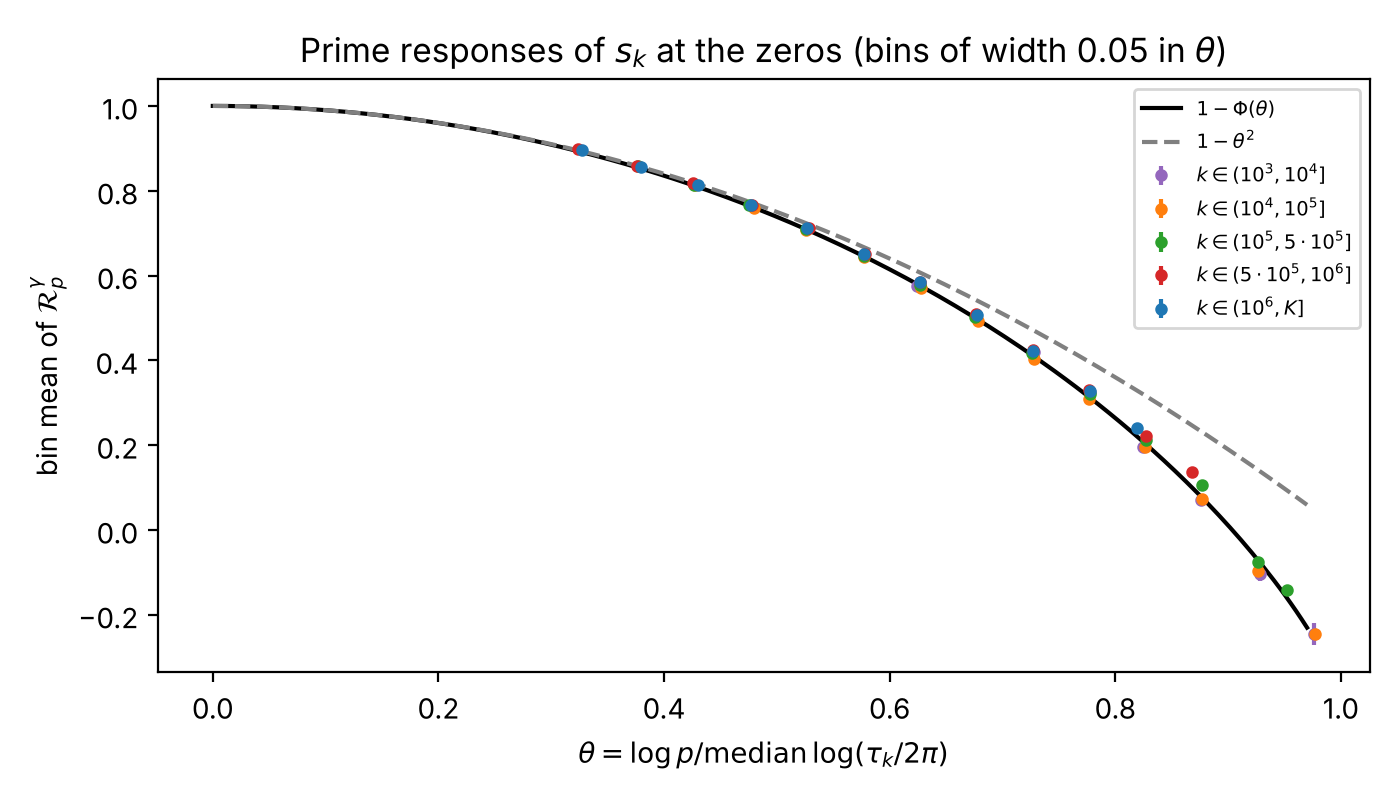
\includegraphics[width=0.86\textwidth]{fig07_response_law.png}
\caption{Bin means of $\Rg_p$ (bars: standard error) against $1-\Phi(\theta)$ (solid) and $1-\theta^2$ (dashed), for five windows of ordinals.}
\label{fig:response_law}
\end{figure}

\begin{figure}[htbp]
\centering
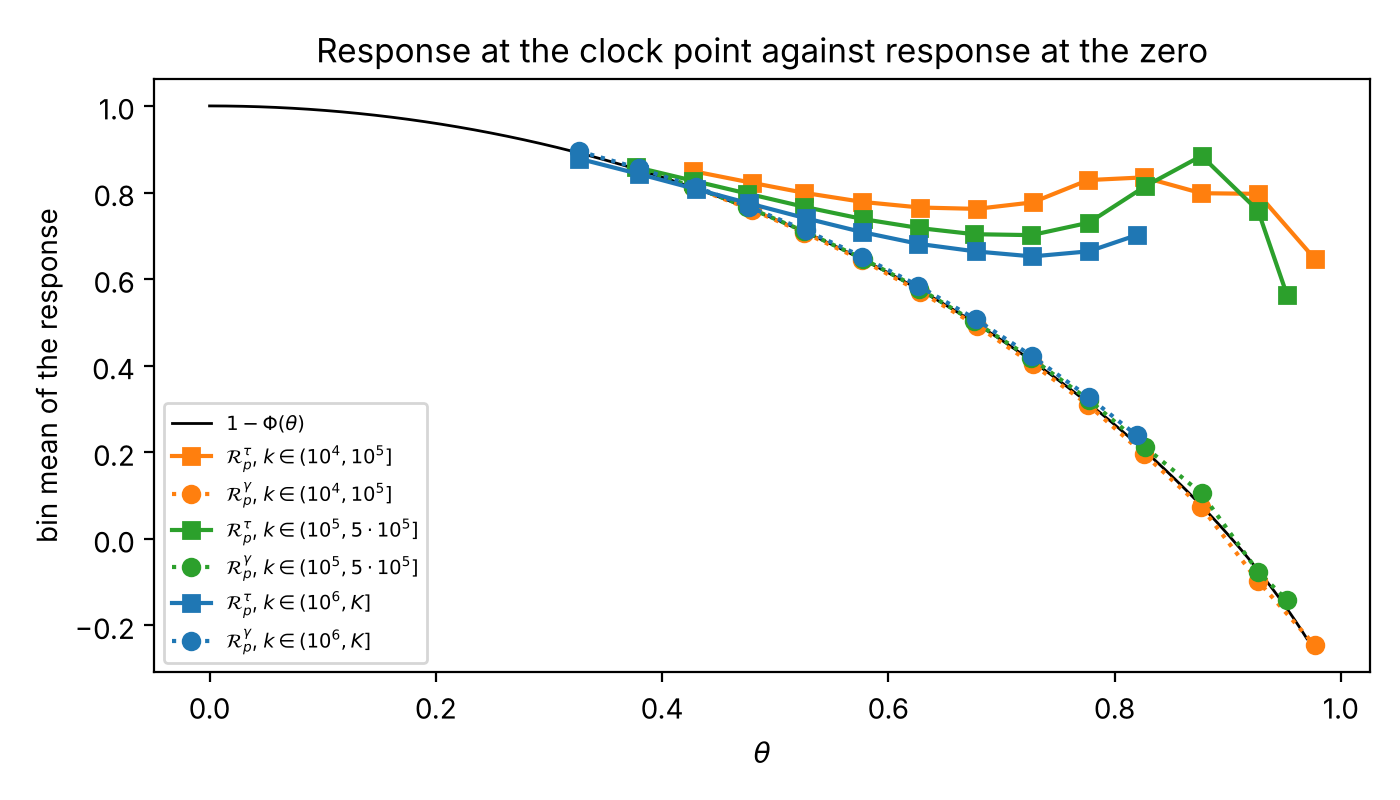
\includegraphics[width=0.86\textwidth]{fig08_response_clock_vs_zero.png}
\caption{Bin means of the response at the clock points, $\Rt_p$ (squares), and at the zeros, $\Rg_p$ (circles), for three windows of ordinals; solid: $1-\Phi(\theta)$.}
\label{fig:response_clock}
\end{figure}

The bin means follow $1-\Phi(\theta)$ and separate from $1-\theta^2$ for $\theta\ge0.6$. The residuals are not noise: in the two top windows every bin mean exceeds the candidate, by about $0.004$ at $\theta\approx0.3$ and $0.02$--$0.035$ at $\theta\approx0.8$--$0.9$, many standard errors, and the excess does not decrease between these two windows. The data are consistent with Conjecture~\CGref{conj:law} only together with a finite-height correction of a few hundredths whose decay is not seen below $\gamma=1.13\cdot10^6$. The response at the clock points follows a different curve, with a plateau near $0.65$--$0.70$ for $\theta\in[0.65,0.80]$ in the top window (Figure~\CGref{fig:response_clock}), as Remark~\CGref{rem:transport} allows.

%======================================================================
\section{Conclusions}
\label{sec:conclusions}

\subsection{What was known}
Before this work, the relation between the RvM clock and the ordinates of the zeros of the Riemann zeta function was known at two levels. Pointwise, $\delta_k=\tau_k-\gamma_k$ is bounded, with $\limsup|\delta_k|\le0.6331$ as an immediate consequence of the bound of Bellotti and Wong \cite{BellottiWong2025}. On average, $s_k$ is asymptotically Gaussian with variance $\frac1{2\pi^2}\log\log T$, by Selberg's formulae for the Gram displacement proved by Korolev \cite{Korolev2012,Korolev2011}: the clock is close to the zeros in $t$, but it misplaces almost every zero by an unbounded number of positions. Selberg's approximation \cite{Selberg1946a,Fujii1974} replaces $S(t)$ by short prime sums in $t$-mean, and Fran\c{c}a--LeClair and LeClair \cite{FrancaLeClair2015,LeClair2021} write the equation of an individual zero with an Euler phase and a growing number of primes, with computations at a fixed number of primes.

\subsection{What this paper adds}
\begin{enumerate}[leftmargin=1.6em]
\item \emph{An exact dictionary between clock-type models and the zeros} (Theorem~\CGref{thm:identity_general}). For any $C^1$ model $F$ of the counting function, averages over the ordinates of the even powers of $k-\frac12-F(\gamma_k)$ are exactly $dF$-averages of $(N-F)^{2j}$ in the continuous variable, corrected only by the sawtooth constant $\frac1{12}$ per zero (for $j=1$) and two boundary terms. No hypothesis on the zeros, no short-interval counts and no monotonicity of $F$ are needed.
\item \emph{The prime information needed by the clock} (Theorem~\CGref{thm:main}). The corrected clock equation $\NO(t)+S_X(t)=k-\frac12$ holds at the true ordinates with mean-square ordinal defect $\frac1{2\pi^2}\log\frac{\log T}{\log X}$ up to $O(1+\sqrt{\log(\log T/\log X)})$. Each factor $e$ in $\log X$ removes $\frac1{2\pi^2}$ from the mean square. The corrected clock assigns the right position to almost all zeros up to a bounded error in mean square if and only if the primes reach a fixed power of the height; a fixed or slowly growing number of primes never does.
\item \emph{An exact finite-height account of the computable clock} (Theorem~\CGref{thm:accounting} and Section~\CGref{sec:computations}). The gain of $\tau_k^X$ is the diagonal response minus a cross term, with no independence assumption, and the residual of $\tau_k^X$ differs from $u_k(X)$ by the explicit transport term $S_X(\gamma_k)-S_X(\tau_k)$. On the first $2\,001\,052$ zeros the growth of the cross term, not a lack of prime information, sets the cutoff that is optimal at a given height.
\item \emph{A sharp conditional target} (Sections~\CGref{sec:conditional} and \CGref{sec:heuristic}). The prime content of $s_k$ at the zeros is reduced, exactly, to a pair correlation shifted by a prime frequency; under two named hypotheses it is $1-\Phi(\theta)$. The data follow this curve up to a systematic excess of a few hundredths.
\end{enumerate}

\subsection{Why a finer knowledge of $\tau_k-\gamma_k$ matters}
The clock is the deterministic part of the ordinates, and $\delta_k$ carries all the arithmetic. Statistics of $\delta_k$ and $s_k$ beyond the variance are statistics of the zeros of the Riemann zeta function that do not depend on an unfolding of the ordinates or on Gram intervals. Theorem~\CGref{thm:identity_general} turns every question about weighted even moments of $k-\frac12-F(\gamma_k)$ into a question about $N-F$ in $t$-mean. Any improvement in the $t$-mean description of $S(t)$ is therefore transferred to the zeros with the constant $\frac1{12}$ and nothing else: sharper forms of Selberg's approximation, prime polynomials longer than $T^{1/2}$, or mixed moments with prime powers would determine the constant left open at fixed $c$, and would extend Theorem~\CGref{thm:main} beyond $c=\frac12$. In the other direction, the identities of Theorem~\CGref{thm:accounting} are exact at the heights where the zeros are known. The measured responses $\Rt_n$, $\Rg_n$ and the cross terms $\Cr_X$ are therefore not approximations but finite-height invariants of the zeros, which any model of the zeros must reproduce. The prime responses of $s_k$ are an example: their bin means follow $1-\Phi(\theta)$, a function that the stationary pair correlation of the zeros does not determine and that requires the shifted correlation \CGeqref{eq:BT_scaled}. Their systematic deviation at the computed heights is a property of the zeros that no current asymptotic statement predicts.

\subsection{Future work}
\begin{question}\label{q:constant}
For fixed $c\in(0,\frac12]$, do the bounded means of $u_k(T^c)^2$ converge, and to $(2\pi^2)^{-1}\log(1/c)$ plus which constant? This needs the mixed Selberg remainders and the prime-power terms, not only upper bounds.
\end{question}

\begin{question}\label{q:large_c}
Can Theorem~\CGref{thm:main} be extended to $c>\frac12$ (the proof uses $X^2\le T$ in the fourth-moment step), and to a cutoff varying at every ordinate, such as $X_k=(\tau_k/2\pi)^c$?
\end{question}

\begin{question}\label{q:prime_bridge}
Can Hypotheses~U and W be proved for moving primes, in the real or the complex form? What is the finite-height correction to $1-\Phi(\theta)$ seen in Table~\CGref{tab:response_bins}? Is there a law for the response $\Rt$ at the clock points, with uniform control of the Gram matrix of Remark~\CGref{rem:matrix_projection}, that would predict the optimal cutoff of the computable clock?
\end{question}

Theorem~\CGref{thm:identity_general} applies to any counting staircase and any $C^1$ model, in particular to the zeros of a primitive Dirichlet $L$-function; an analogue of Theorem~\CGref{thm:main} would additionally need Selberg's approximation for $L(s,\chi)$ \cite{Selberg1946b,Fujii1974} and uniformity in the conductor.

\section*{Declaration of competing interest}
The author declares no competing interests.

\section*{Data availability}
All programs, the input-generation script with its certificates, the numerical outputs (CSV and JSON) and the figures are in the public GitHub repository \texttt{ordinal\_prime\_cutoff\_v7} (link to be inserted). The ordinates are Odlyzko's table \cite{OdlyzkoTables}; the two input files (arrays of $2\,001\,052$ little-endian double-precision numbers) are regenerated from that table by \texttt{make\_inputs\_v7.py}. Their SHA-256 identifiers are \texttt{fafb9436ce6a\ldots9e0015b3e945fe0ac} (ordinates) and \texttt{b4c6758f0aef\ldots 266091f713faa9504} (clock). The computations used Python 3.13.16, NumPy 2.5.3, SciPy 1.18.1, Matplotlib 3.11.2 and mpmath 1.3.0.

\section*{Declaration of generative AI and AI-assisted technologies in the writing process}
During the preparation of this work the author used an AI assistant (Claude, Anthropic) to edit the text, check proofs and write analysis programs. The author reviewed and edited the content and takes full responsibility for it.

%======================================================================
\begin{thebibliography}{99}

\bibitem{BellottiWong2025}
C. Bellotti, P.-J. Wong, Improved estimates for the argument and zero-counting function of the Riemann zeta-function, Math. Comp. (2025), \href{https://doi.org/10.1090/mcom/4133}{https://doi.org/10.1090/mcom/4133}.

\bibitem{Billingsley1995}
P. Billingsley, Probability and Measure, third ed., Wiley, New York, 1995.

\bibitem{Corless1996}
R.M. Corless, G.H. Gonnet, D.E.G. Hare, D.J. Jeffrey, D.E. Knuth, On the Lambert $W$ function, Adv. Comput. Math. 5 (1996) 329--359, \href{https://doi.org/10.1007/BF02124750}{https://doi.org/10.1007/BF02124750}.

\bibitem{Folland1999}
G.B. Folland, Real Analysis: Modern Techniques and Their Applications, second ed., Wiley, New York, 1999.

\bibitem{FrancaLeClair2014}
G. Fran\c{c}a, A. LeClair, Statistical and other properties of Riemann zeros based on an explicit equation for the $n$-th zero on the critical line, preprint, arXiv:1307.8395, 2013, \href{https://doi.org/10.48550/arXiv.1307.8395}{https://doi.org/10.48550/arXiv.1307.8395}.

\bibitem{FrancaLeClair2015}
G. Fran\c{c}a, A. LeClair, Transcendental equations satisfied by the individual zeros of Riemann $\zeta$, Dirichlet and modular $L$-functions, Commun. Number Theory Phys. 9 (1) (2015) 1--50, \href{https://doi.org/10.4310/CNTP.2015.v9.n1.a1}{https://doi.org/10.4310/CNTP.2015.v9.n1.a1}.

\bibitem{Fujii1974}
A. Fujii, On the zeros of Dirichlet $L$-functions. I, Trans. Amer. Math. Soc. 196 (1974) 225--235, \href{https://doi.org/10.1090/S0002-9947-1974-0349603-2}{https://doi.org/10.1090/S0002-9947-1974-0349603-2}.

\bibitem{Gonek1993}
S.M. Gonek, An explicit formula of Landau and its applications to the theory of the zeta-function, in: A Tribute to Emil Grosswald: Number Theory and Related Analysis, Contemp. Math., vol. 143, Amer. Math. Soc., Providence, RI, 1993, pp. 395--413, \href{https://doi.org/10.1090/conm/143/1210528}{https://doi.org/10.1090/conm/143/1210528}.

\bibitem{GrahamKolesnik1991}
S.W. Graham, G. Kolesnik, Van der Corput's Method of Exponential Sums, London Math. Soc. Lecture Note Ser., vol. 126, Cambridge University Press, Cambridge, 1991, \href{https://doi.org/10.1017/CBO9780511661976}{https://doi.org/10.1017/CBO9780511661976}.

\bibitem{HasanalizadeShenWong2022}
E. Hasanalizade, Q. Shen, P.-J. Wong, Counting zeros of the Riemann zeta function, J. Number Theory 235 (2022) 219--241, \href{https://doi.org/10.1016/j.jnt.2021.06.032}{https://doi.org/10.1016/j.jnt.2021.06.032}.

\bibitem{Korolev2011}
M.A. Korolev, Gram's law and the argument of the Riemann zeta function, preprint, arXiv:1106.0516, 2011, \href{https://doi.org/10.48550/arXiv.1106.0516}{https://doi.org/10.48550/arXiv.1106.0516}.

\bibitem{Korolev2012}
M.A. Korolev, On Gram's law in the theory of the Riemann zeta function, Izv. Math. 76 (2) (2012) 275--309, \href{https://doi.org/10.1070/IM2012v076n02ABEH002583}{https://doi.org/10.1070/IM2012v076n02ABEH002583}.

\bibitem{Landau1912}
E. Landau, \"Uber die Nullstellen der Zetafunktion, Math. Ann. 71 (1912) 548--564, \href{https://doi.org/10.1007/BF01456808}{https://doi.org/10.1007/BF01456808}.

\bibitem{LeClair2021}
A. LeClair, Riemann hypothesis and random walks: the zeta case, Symmetry 13 (11) (2021) 2014, \href{https://doi.org/10.3390/sym13112014}{https://doi.org/10.3390/sym13112014}.

\bibitem{Littlewood1924}
J.E. Littlewood, On the zeros of the Riemann zeta-function, Proc. Cambridge Philos. Soc. 22 (1924) 295--318, \href{https://doi.org/10.1017/S0305004100014225}{https://doi.org/10.1017/S0305004100014225}.

\bibitem{Mertens1874}
F. Mertens, Ein Beitrag zur analytischen Zahlentheorie, J. Reine Angew. Math. 78 (1874) 46--62, \href{https://doi.org/10.1515/crll.1874.78.46}{https://doi.org/10.1515/crll.1874.78.46}.

\bibitem{MontgomeryVaughan1974}
H.L. Montgomery, R.C. Vaughan, Hilbert's inequality, J. Lond. Math. Soc. (2) 8 (1974) 73--82, \href{https://doi.org/10.1112/jlms/s2-8.1.73}{https://doi.org/10.1112/jlms/s2-8.1.73}.

\bibitem{OdlyzkoTables}
A.M. Odlyzko, Tables of zeros of the Riemann zeta function: the first 2,001,052 zeros, accurate to within $4\cdot10^{-9}$, \url{https://www-users.cse.umn.edu/~odlyzko/zeta_tables/}, accessed 17 October 2026.

\bibitem{Selberg1946a}
A. Selberg, Contributions to the theory of the Riemann zeta-function, Arch. Math. Naturvid. 48 (5) (1946) 89--155.

\bibitem{Selberg1946b}
A. Selberg, Contributions to the theory of Dirichlet's $L$-functions, Skr. Norske Vid.-Akad. Oslo I 1946 (3) (1946) 2--62.

\bibitem{Soshnikov2002}
A. Soshnikov, Gaussian limit for determinantal random point fields, Ann. Probab. 30 (1) (2002) 171--187, \href{https://doi.org/10.1214/aop/1020107764}{https://doi.org/10.1214/aop/1020107764}.

\bibitem{Titchmarsh1986}
E.C. Titchmarsh, The Theory of the Riemann Zeta-Function, second ed., revised by D.R. Heath-Brown, Clarendon Press, Oxford, 1986.

\bibitem{Trudgian2014}
T.S. Trudgian, An improved upper bound for the argument of the Riemann zeta-function on the critical line II, J. Number Theory 134 (2014) 280--292, \href{https://doi.org/10.1016/j.jnt.2013.07.017}{https://doi.org/10.1016/j.jnt.2013.07.017}.

\end{thebibliography}

\end{document}
